\documentclass[letter,11pt]{article}
\usepackage{amsmath}
\usepackage{tikz}
\usepackage{graphicx}
\makeatletter
\def\maxwidth{\ifdim\Gin@nat@width>\linewidth\linewidth\else\Gin@nat@width\fi}
\def\maxheight{\ifdim\Gin@nat@height>\textheight\textheight\else\Gin@nat@height\fi}
\makeatother
\setkeys{Gin}{width=\maxwidth,height=\maxheight,keepaspectratio}
\usepackage[spanish,es-tabla]{babel}
%\usepackage{draftwatermark}
%\SetWatermarkText{Preliminar}
\usepackage{gensymb}
\usepackage{parskip}
\usepackage[hidelinks]{hyperref}
\urlstyle{same}
\usepackage{caption}
\captionsetup{justification=justified,format=plain,font=small,labelfont=bf,margin=50pt}
\captionsetup[table]{name=\textbf{Tabla},labelsep=period}
\captionsetup[figure]{name=\textbf{Figura},labelsep=period}
\usepackage{fancyhdr}
\pagestyle{fancy}
\fancyhf{}
\usepackage[top=1.3cm,bottom=1.3cm,left=2.5cm,right=2.5cm]{geometry}
\usepackage{helvet}
\renewcommand{\familydefault}{\sfdefault}
\usepackage{multirow}
\usepackage{ragged2e}
\newcommand{\sietepuntos}{\fontsize{7pt}{\baselineskip}\selectfont}
\newcommand{\cincopuntos}{\fontsize{6pt}{\baselineskip}\selectfont}
\newcommand{\ochopuntos}{\fontsize{8.8pt}{\baselineskip}\selectfont}
\newcommand{\nuevepuntos}{\fontsize{9.6pt}{\baselineskip}\selectfont}
\usepackage{color,colortbl}
\definecolor{Gray}{rgb}{0.801,0.801,0.801}
\definecolor{Gray1}{rgb}{0.790,0.790,0.790}
\definecolor{Gray2}{rgb}{0.830,0.830,0.830}
\definecolor{Gray3}{rgb}{0.870,0.870,0.870}
\definecolor{Gray4}{rgb}{0.910,0.910,0.910}
%\addtolength{\headheight}{8.5\baselineskip}
\setlength{\headheight}{70pt}
\setlength{\footskip}{35pt}%5
\setlength{\textheight}{638pt}%658
\fancyhead[CE,CO]{
\includegraphics[height=1.5cm]{logoifop.png}\\ \sietepuntos INSTITUTO DE FOMENTO PESQUERO / DIVISION INVESTIGACION PESQUERA}
\fancyheadoffset{0.01cm}
\renewcommand{\headrulewidth}{0.5pt}
\renewcommand{\footrulewidth}{0.5pt}
\fancyfoot[CO,CE]{\cincopuntos \vspace{-0.6cm} \thepage \\ \vspace{0.4cm} %-------------------------------------------------------------------------------\\
\vspace{-0.2cm} \cincopuntos CONVENIO DE DESEMPE\~{N}O 2021 IFOP/SUBSECRETAR\'IA DE ECONOM\'IA Y EMT \\ \vspace{-0.1cm} REPORTE T\'ECNICO. ANCHOVETA Y SARDINA ESPA\~{N}OLA, REGI\'ON DE ARICA Y PARINACOTA A LA REGI\'ON DE ANTOFAGASTA, 2022}
\author{}
\date{\vspace{-2.5em}}

\begin{document}

\begin{titlepage}
\begin{tikzpicture}
\node[anchor=south west,inner sep=0] at (0,0) {
\includegraphics[height=22.3cm,width=22cm,viewport=29 26 148 274]{portada1.pdf}};
%\node[anchor=south west,inner sep=0] at (0,0) {
\includegraphics[height=22.3cm,width=22cm,viewport=70 74 318 698]{portada1.pdf}};
\node[text width=8cm] at (14.56,16.60) {\large \textbf{REPORTE T\'ECNICO}};
\node[text width=8cm] at (14.37,16.13) {\ochopuntos Convenio de Desempe\~{n}o 2021};
\node[text width=8cm] at (10.58,15.46) {\nuevepuntos Estatus y posibilidades de explotaci\'on biol\'ogicamente};
\node[text width=8cm] at (11.62,15.08) {\nuevepuntos sustentables de anchoveta y sardina espa\~{n}ola,};
\node[text width=10cm] at (9.60,14.72) {\nuevepuntos Regi\'on de Arica y Parinacota a la Regi\'on de Antofagasta, a\~{n}o 2022};
\node[text width=10cm] at (11.66,14.00) {\footnotesize \textbf{SUBSECRETAR\'IA DE ECONOM\'IA Y EMT / Julio 2021}};
\end{tikzpicture}
\end{titlepage}

\begin{titlepage}
\begin{tikzpicture}
\node[anchor=south west,inner sep=0] at (0,0) {
\includegraphics[height=22.3cm,width=22cm,viewport=70 74 318 698]{portada2.pdf}};
\node[text width=8cm] at (15.59,17.85) {\large \textbf{REPORTE T\'ECNICO}};
\node[text width=8cm] at (15.43,17.38) {\ochopuntos Convenio de Desempe\~{n}o 2021};
\node[text width=8cm] at (11.85,16.50) {\nuevepuntos Estatus y posibilidades de explotaci\'on biol\'ogicamente};
\node[text width=8cm] at (12.86,16.09) {\nuevepuntos sustentables de anchoveta y sardina espa\~{n}ola,};
\node[text width=10cm] at (10.85,15.72) {\nuevepuntos Regi\'on de Arica y Parinacota a la Regi\'on de Antofagasta, a\~{n}o 2022};
\node[text width=10cm] at (12.86,14.85) {\footnotesize \textbf{SUBSECRETAR\'IA DE ECONOM\'IA Y EMT / Julio 2021}};
\node[text width=8cm] at (17.07,12.15) {\footnotesize \textbf{REQUERENTE}};
\node[text width=8cm] at (14.10,11.85) {\ochopuntos \textbf{SUBSECRETAR\'IA DE ECONOM\'IA Y}};
\node[text width=8cm] at (14.46,11.49) {\ochopuntos \textbf{EMPRESAS DE MENOR TAMA\~{N}O}};
\node[text width=8cm] at (15.29,10.70) {\ochopuntos Subsecretario de Econom\'ia y};
\node[text width=8cm] at (15.38,10.37) {\ochopuntos Empresas de Menor Tama\~{n}o};
\node[text width=8cm] at (15.36,10.00) {\ochopuntos \textbf{Julio Alberto Pertuze Salas}};
\node[text width=8cm] at (17.55,9.15) {\footnotesize \textbf{EJECUTOR}};
\node[text width=8cm] at (12.65,8.79) {\footnotesize \textbf{INSTITUTO DE FOMENTO PESQUERO, IFOP}};
\node[text width=8cm] at (16.83,7.97) {\ochopuntos Director Ejecutivo};
\node[text width=8cm] at (16.52,7.61) {\ochopuntos \textbf{Luis Parot Donoso}};
\node[text width=8cm] at (13.89,6.87) {\ochopuntos Jefe (I) Divisi\'on Investigaci\'on Pesquera};
\node[text width=8cm] at (16.75,6.46) {\ochopuntos \textbf{Sergio Lillo Vega}};
\node[text width=8cm] at (16.07,5.25) {\footnotesize \textbf{JEFE DE PROYECTO}};
\node[text width=8cm] at (15.27,4.87) {\ochopuntos Juan Carlos Quiroz Espinoza};
\node[text width=8cm] at (17.66,4.05) {\footnotesize \textbf{AUTORES}};
\node[text width=8cm] at (14.95,3.67) {\ochopuntos Fernando Esp\'indola Rebolledo};
\node[text width=8cm] at (15.44,3.32) {\ochopuntos Mar\'a Jos\'e Z\'u\~{n}iga Basualto};
\node[text width=8cm] at (15.53,2.94) {\ochopuntos Doris Bucarey Sep\'ulvedad};
\node[text width=8cm] at (15.17,2.61) {\ochopuntos Juan Carlos Quiroz Espinoza};
\end{tikzpicture}
\end{titlepage}


{
\setcounter{tocdepth}{3}
\tableofcontents
}

\newpage
\listoffigures

\newpage
\listoftables

\newpage

\section{RESUMEN EJECUTIVO}

El presente reporte técnico contiene los resultados de la proyecci\'on del stock
de anchoveta (\textit{Engraulis ringens}) del sur de Per\'u y norte de Chile
(regi\'on de Arica y Parinacota a regi\'on de Antofagasta), para el primer y
segundo hito de asesor\'ia cient\'ifica, y los supuestos empleados en cada
uno de los hitos para el establecimiento de la Captura Biol\'ogicamente
Acepatable (CBA). Estos resultados fueron presentados en la cuarta sesi\'on del Comit\'e
Cient\'ifico T\'ecnico (CCT) como parte del \textit{Taller de Datos y Modelos}, el cu\'al se
enmarca en la reducci\'on de brechas en consistencia con los temas relevados en el
Programa de Mejoramiento Continuo de la Calidad de la Asesor\'ia Cient\'ifica (PMCCAC).\\

Los an\'alisis desarrollados en el presente reporte buscan reducir la
incertidumbre en la proyecci\'on del stock que genera la recomendaci\'on de
cuota en cada uno de los hitos de asesor\'ia cient\'ifica para el establecimiento de la
CBA, originada tanto por el patr\'on retrospectivo que se observan en los reclutamientos,
que tiende a sobreestimar los reclutamientos del \'ultimo semestre de la evaluaci\'on, como
tambi\'en, por los supuestos de reclutamientos promedios (longitud de la serie) que son usados
durante la proyecci\'on del stock de anchoveta. Otro aspecto a considerar durante la
proyecci\'on del stock en el primer hito (4 semestres) de asesor\'ia, es que en el primer
y segundo semestre de la proyecci\'on la captura es conocida, por la tanto es posible
resolver la mortalidad por pesca para cada flota.\\

En este sentido, se evaluaron ocho escenarios en la proyecci\'on del
stock de anchoveta para cada hito de asesor\'ia. Adem\'as, se evalu\'o proyectar
el stock de anchoveta durante tres semestres, es decir, se incorpor\'o un semestre 
de informaci\'on en la evaluaci\'on de stock. Para el primer hito de asesor\'ia, los
resultados indican que la CBA anual deber\'ia fluctuar entre las 776 a 724 mil toneladas
y un mill\'on 166 mil toneladas a 648 mil toneladas para la proyecci\'on de cuatro y
tres semestres, respectivamente. Para el segundo hito de asesor\'ia, la CBA anual deber\'ia
fluctuar entre un mill\'on 109 mil toneladas a 595 mil toneladas. En t\'erminos generales,
el grupo de edad 1 (6 meses de edad) es el que aporta el mayor porcentaje de individuos en
la captura, con valores que var\'ian entre un 74\% a un 91\% y un 71\% a un 89\% para el primer
(4 semestres) y segundo (2 semestres) hito de asesor\'ia, respectivamente. Esto implica, que
para el primer hito de asesor\'ia, la CBA anual estimada depende de los supuestos de reclutamientos promedios que ingresan durante la proyecci\'on, es decir, la longitud de la serie usada para
calcular los reclutamientos promedios. En cambio, para el segundo hito de asesor\'ia, la CBA
anual estimada depende principalmente si el \'ultimo reclutamiento estimado por el modelo es
penalizado o no, y secundariamente del m\'etodo usado para penalizar el \'ultimo reclutamiento
estimado por el modelo, encontr\'andose diferencias de hasta cincuenta toneladas entre un m\'etodo
y otro.\\


\clearpage
\pagebreak


\section{ANTECEDENTES}

\subsection{Desembarques}


La historia de la pesquer\'ia del stock de anchoveta compartido entre el
sur de Per\'u y norte de Chile, comienza con leves desembarques ocurridos
en 1984 y a contar de 1986 se incrementan considerablemente hasta el a\~{n}o
1994 (\textbf{Tabla \ref{Tab0}}; \textbf{Figura \ref{Fig0}}), los m\'as
altos desembarques ocurren entre los a\~{n}os 1994 al 2002. Desde el a\~{n}o
2004 al primer semestre 2013 estos muestran una tendencia de descenso
con m\'aximos relativos. El desembarque por pa\'is muestra un cambio de
dominancia, entre los a\~{n}os 1986 al 2004 se puede se\~{n}alar que el mayor
desembarque fue realizado en el norte de Chile. Sin embargo, entre el 2005 al 2009
los mayores desembarques se realizaron en sur de Per\'u. Entre las causas
probables de la dominancia peruana del desembarque se encuentra el
aumento del esfuerzo de pesca en la pesquer\'ia del sur del Per\'u debido a
la mayor disponibilidad de anchoveta en dicha \'area seg\'un lo informado
por IMARPE en el 12$^{do}$ taller de evaluaci\'on conjunta de IFOP e IMARPE,
2008 (Serra y Canales, 2013). Y desde el a\~{n}o 2010 a diciembre del 2013
el desembarque chileno ha dominado el desembarque total del stock
anchoveta. Se postula que el incremento del desembarque chileno en el
a\~{n}o 2011 habr\'ia estado asociado a un desplazamiento de la anchoveta del
sur de Per\'u hacia el norte de Chile, evidenci\'andose un incremento del
desembarque particularmente en la zona de Arica (B\"ohm \textit{et al}.,
2013).\\


\vspace{0.5cm}
\begin{figure}[htb!]
 \centering
 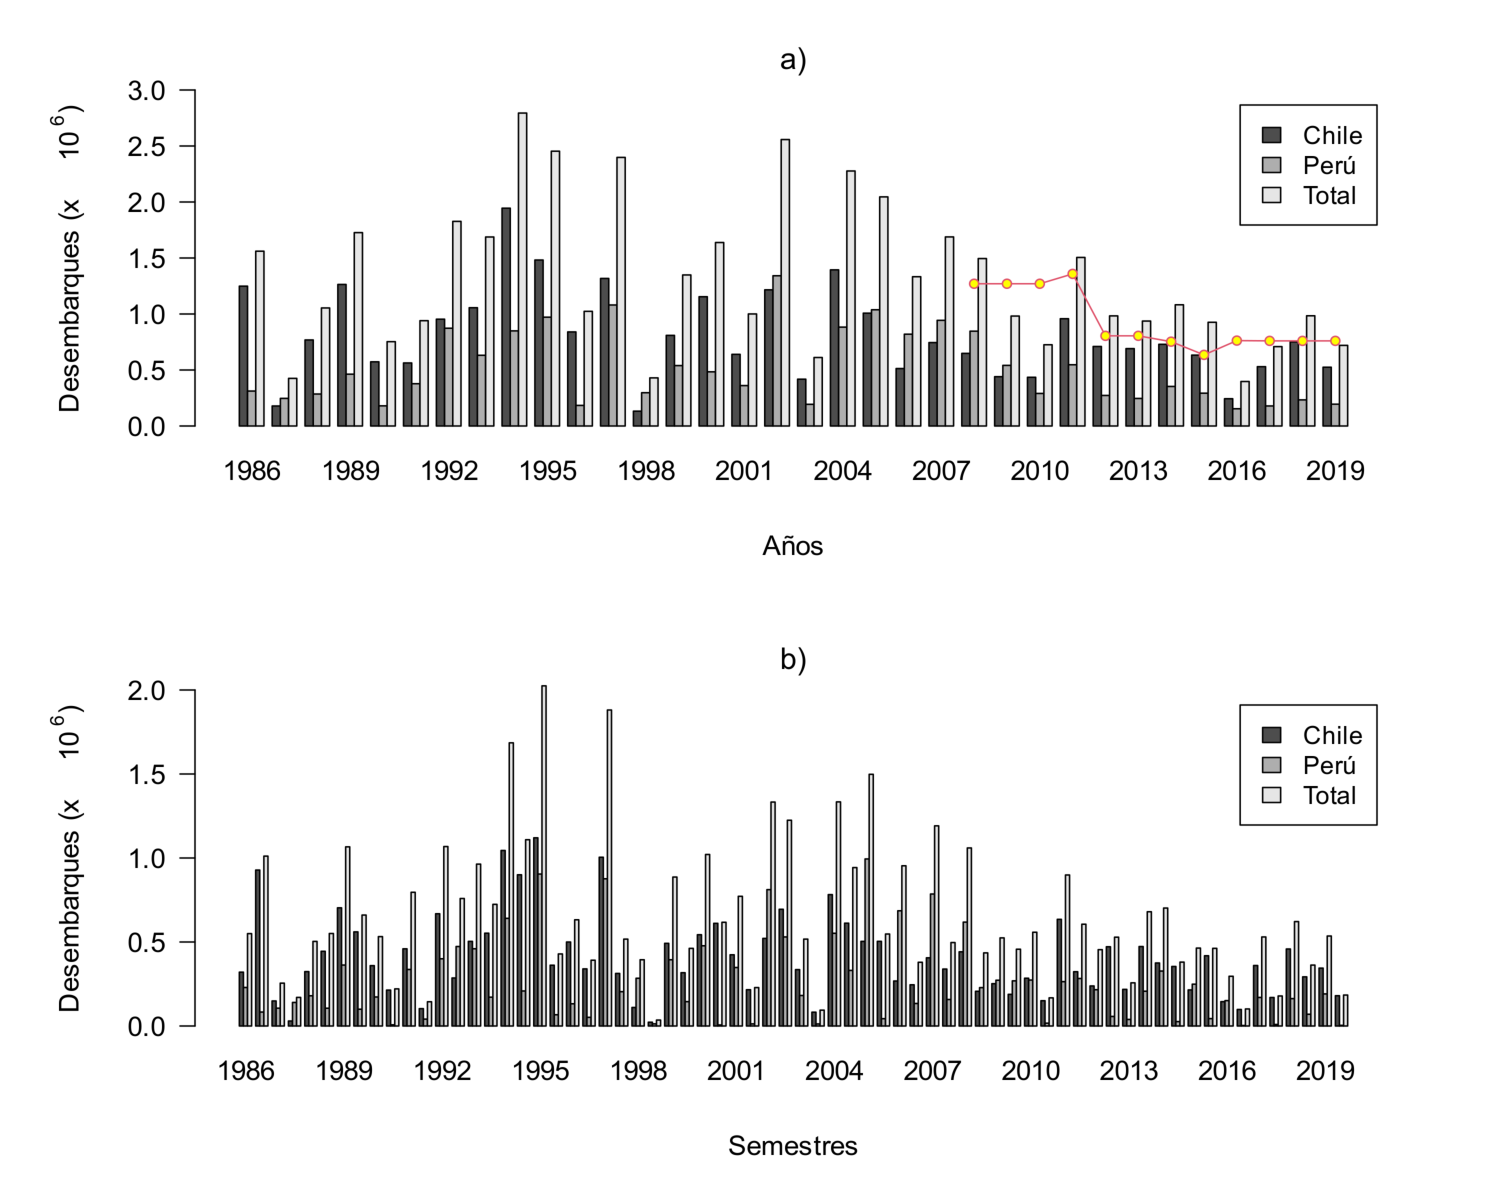
\includegraphics[width=17.3cm,height=10.1cm]{fig/figura0.pdf}
 \caption{Desembarques anuales y semestrales para Chile, Per\'u y Total del stock de anchoveta distribuido entre 16\degree LS - 24\degree LS (1986 - 2019). Los puntos amarillos representan la cuota chilena. En el panel superior (a) se muestra el desembarque en escala anual y en el panel inferior (b) en escala semestral.}
 \label{Fig0}
\end{figure}
\vspace{0.5cm}



M\'as recientemente y de acuerdo a las estad\'isticas oficiales, el primer y
segundo semestre del 2014 se capturaron en Chile 375.1 mil y 354.3 mil
toneladas, respectivamente. Por su parte, en el sur del Per\'u y de
acuerdo a lo informado en Oficio PRODUCE 100-59-2015, el desembarque
acumulado de enero a octubre hab\'ia sido de 336.7 mil toneladas, de las
cuales solo 26 mil toneladas fueron capturadas en el segundo semestre.
Si se considera adem\'as que producto de este oficio la captura de
anchoveta fue prohibida en la zona sur del Per\'u en noviembre y diciembre
2014 debido a la gran presencia de reclutas, se deduce entonces que la
captura en esta regi\'on pudo haber alcanzado 310 mil toneladas durante el
primer semestre del 2014. De esta forma, el desembarque total 2014 se
estima en 1.082 millones de toneladas (\textbf{Tabla \ref{Tab0}}) el
cual se traduce un alza del 15\% respecto del a\~{n}o 2013, y el desembarque
del 2015 disminuy\'o en un 1\% con respecto al 2013. Y el desembarque del
2015 se tradujo en una disminuci\'on del 14\% con respecto al del 2014.
Sin embargo, el desembarque durante el 2016 se redujo fuertemente,
alcanzando 397 mil toneladas para ambos pa\'ises. Y finalmente, en el a\~{n}o
2017 el desembarque aumento a 708 mil toneladas. Cerrando el a\~{n}o 2018,
se registra un desembarque total de 971.1 mil toneladas, un 37\%
superior a lo registrado en el 2017. Desde el 2016 hasta el 2018 se
viene registrando un aumento constante de los desembarques, pasando de
397.4, 708.7, 984.1 mil toneladas, respectivamente
(\textbf{Figura \ref{Fig0}}). \\



\newpage



\vspace{0.5cm}
\begin{table}[htb!]
 \caption{Desembarques del stock de anchoveta 16\degree - 24\degree LS 1986-2019.}
 \label{Tab0}
 \centering
 \small
 \begin{tabular}{cccc}
 \hline\noalign{\vskip 0.1cm}
 A\~{n}o & Sur Per\'u & Norte Chile & Total \\
 \hline\noalign{\vskip 0.1cm}
 1986  &  321.2  &  1248.7  &  1560.9  \\
 1987  &  246.4  &   178.8  &   425.2  \\
 1988  &  285.6  &   768.5  &  1054.1  \\
 1989  &  462.8  &  1263.8  &  1726.6  \\
 1990  &  179.9  &   573.1  &   753.0  \\
 1991  &  377.5  &   562.8  &   940.3  \\
 1992  &  873.2  &   953.9  &  1827.1  \\
 1993  &  631.4  &  1056.2  &  1687.1  \\
 1994  &  849.2  &  1945.0  &  2794.2  \\
 1995  &  971.5  &  1482.1  &  2453.6  \\
 1996  &  183.8  &   840.0  &  1023.8  \\
 1997  & 1080.6  &  1317.4  &  2398.0  \\  
 1998  &  297.0  &   132.7  &   429.7  \\
 1999  &  539.4  &   809.2  &  1348.6  \\
 2000  &  483.8  &  1154.4  &  1638.2  \\
 2001  &  360.8  &   639.8  &  1000.6  \\
 2002  & 1341.6  &  1216.0  &  2557.6  \\
 2003  &  193.7  &   417.9  &   611.6  \\
 2004  &  882.8  &  1394.1  &  2276.9  \\
 2005  & 1037.9  &  1007.7  &  2045.6  \\
 2006  &  819.8  &   513.1  &  1332.9  \\
 2007  &  943.4  &   744.8  &  1688.2  \\
 2008  &  846.8  &   648.2  &  1495.0  \\
 2009  &  541.3  &   440.2  &   981.5  \\
 2010  &  290.5  &   435.0  &   725.5  \\
 2011  &  546.8  &   958.0  &  1504.8  \\
 2012  &  272.9  &   710.1  &   983.0  \\
 2013  &  246.0  &   691.0  &   937.0  \\
 2014  &  353.0  &   729.4  &  1082.4  \\
 2015  &  293.0  &   633.0  &   926.0  \\
 2016  &  154.0  &   243.4  &   397.4  \\
 2017  &  179.0  &   529.7  &   708.7  \\
 2018  &  220.0  &   751.1  &   971.1  \\
 2019  &  195.0  &   524.9  &   719.9  \\
 \hline
 \end{tabular}
\end{table}
\vspace{0.5cm}

\newpage

\subsection{\'Indices de abundancia}


Las estimaciones de biomasa desovante disponible para la evaluaci\'on de stock
se entregan en la \textbf{Tabla \ref{Tab1}}, el \'indice de biomasa desovante utilizado
corresponde al reportado por Claramunt \textit{et al}. (2014). En el 2014 la estimaci\'on
de biomasa desovante alcanz\'o un valor de 399 mil toneladas. En el 2015 la
estimaci\'on de biomasa desovante subi\'o a 436 mil toneladas,
luego en el 2016 fue de 461 mil toneladas y en el 2017 de 201 mil
toneladas, lo que representa una disminuci\'on del 56\% con respecto al
2016. En el 2018 la biomasa desovante estimada aumento a las 799 mil
toneladas y en el 2019 esta fue de 645 mil toneladas. Sin embargo, en el
2020 este valor alcanz\'o las 297 mil toneladas. En la
\textbf{Tabla \ref{Tab1}} se muestran los \'indices provenientes de los
cruceros ac\'usticos por a\~{n}o e incluye: i) la biomasa total del sur de Per\'u
(1990 al 2019) y la biomasa total del norte de Chile (Castillo \textit{et al}., 2009,
2010, 2011, 2012, 2013). Para el crucero del norte de Chile se incluye tambi\'en la
estructura de tama\~{n}os disponible para la abundancia total (2000-2002 y 2007-2019)
y la fecha en que se desarroll\'o el crucero ac\'ustico. La actualizaci\'on de
los registros peruanos se efectu\'o a trav\'es de los Talleres IMARPE-IFOP
de Evaluaci\'on Conjunta del Stock de Anchoveta del Sur de Per\'u y Norte de
Chile, el \'ultimo realizado entre el 3 y 7 de diciembre del 2018 en el
Club Alem\'an, Valpara\'iso, Chile.\\


En enero 2015, IMARPE report\'o en la zona sur del Per\'u una biomasa
total de 534 mil toneladas, de las cuales el 94\% estaba compuesta por reclutas
(Oficio PRODUCE 100-556-2014), individuos menores a
11.5 cm. Asimismo, poco antes y en diciembre del 2014 IFOP hab\'ia
registrado una biomasa de 410 mil toneladas cuya incidencia de reclutas
alcanzaba el 60\% en peso. Y para el 2016 se estima una biomasa total de
307 mil toneladas para el norte de Chile y en el 2017 este valor fue de
105 mil toneladas. Sin embargo, este valor sube dr\'asticamente a 793 mil
toneladas de biomasa total en el 2018, lo que representa un aumento de
m\'as de seis veces de magnitud. Pero en el 2019 este valor cae
dr\'asticamente a las 230 mil toneladas. Las estructuras de tallas de los
cruceros ac\'usticos de anchoveta est\'an disponibles desde el 2000 hasta
2002 y desde el 2007 hasta el 2019. Esta informaci\'on es relevante dado
por la presencia de individuos de menor tama\~{n}o (individuos desde los 2.5 cm),
dando cuenta de los reclutas que est\'an ingresando a la pesquer\'ia, y por el
extenso periodo que abarca esta informaci\'on (\textbf{Figura \ref{Fig01}}).\\


La \textbf{Figura \ref{Fig02}} muestra los \'indices utilizados en la 
evaluaci\'on de stock al segundo semestre del 2019. En el caso de
la biomasa total ac\'ustica del Per\'u, representa la fracci\'on
correspondiente a la regi\'on sur de Per\'u (16-18\degree 21`L.S.). En el
caso de la biomasa ac\'ustica de Chile representa la totalidad de la
biomasa estimada desde los 18\degree 21' hasta los 24\degree L.S. Las
estimaciones hechas a fines de primavera de los a\~{n}os 2014, 2015 y 2016
se han registrado altos valores, con un promedio de 334 ($\pm$) 66) mil
toneladas, un gran porcentaje de estas biomasas corresponde a la
fracci\'on juvenil del stock. Durante el 2017 este valor cae a 105 mil
toneladas para luego expandirse a 793 mil toneladas durante el 2018,
valor m\'as alto de la serie hist\'orica. Sin embargo, este valor cae a 230
mil toneladas en el 2019. Por otra parte, la biomasa desovante estimada
en el segundo semestre del 2017 alcanz\'o un valor de 201 mil toneladas, el
valor m\'as bajo de toda la serie hist\'orica estimada por el m\'etodo de
producci\'on diaria de huevos para la anchoveta del norte de Chile. Pero la
estimaci\'on hecha en el 2018, la biomasa desovante alcanz\'o un valor de
799 mil toneladas, mostrando un aumento de casi cuatro veces con respecto al valor
observado en el 2017 (\textbf{Figura \ref{Fig02}}). Sin embargo, este
valor cae levemente en el 2019 a 651 mil toneladas.\\


\vspace{0.5cm}
\begin{table}[htb!]
 \caption{Biomasa estimada a trav\'es del M\'etodo de Producci\'on de Huevos (MPH) y cruceros ac\'usticos del stock de anchoveta del sur de Per\'u y norte de Chile.}
 \label{Tab1}
 \centering
 \small
 \begin{tabular}{lrrr}
 \hline\noalign{\vskip 0.1cm}
 A\~{n}o & MPH & Ac\'ustica Per\'u & Ac\'ustica Chile \\
 \hline\noalign{\vskip 0.1cm}
  1990  &  \---   &  187.000  &  \---  \\
 1991  &  \---   &   558.000  &  \---  \\
 1992  &  314.232  &   482.000  &  \---  \\
 1993  &  \---   &   893.000  &  \---  \\
 1994  &  \---   &   744.000  &  \---  \\
 1995  &  465.696  &  2.667.000  &  \---  \\
 1996  &  253.356  &   648.000  &  385.881  \\
 1997  &  744.838  &   745.000  &  \---  \\  
 1998  &  \---   &  1.306.000  &  957.868  \\
 1999  &  973.292  &   178.000  &  \---  \\
 2000  &  608.087  &   522.000  &  959.791  \\
 2001  &  765.885  &   199.000  &  317.977  \\
 2002  & 1.503.911  &  1008.000  &  \---  \\
 2003  & 1.238.731  &   839.000  &  \---  \\
 2004  &  668.979  &   682.000  &  \---  \\
 2005  & 1.520.754  &  1.375.000  &  \---  \\
 2006  & 1.081.156  &   283.000  &  \---  \\
 2007  &  240.727  &  1.318.000  &  713.012  \\
 2008  &  532.132  &   554.000  &  135.550  \\
 2009  &  287.916  &   425.000  &  456.341  \\
 2010  &  \---   &  1.274.000  &  253.861  \\
 2011  &  795.056  &   613.000  &  170.405  \\
 2012  &  672.077  &  2.271.000  &  299.520  \\
 2013  &  520.336  &  2.013.000  &  163.002  \\
 2014  &  399.605  &   884.000  &  410.660  \\
 2015  &  436.014  &   534.000  &  285.644  \\
 2016  &  461.000  &   370.000  &  307.129  \\
 2017  &  201.178  &  1.487.000  &  105.841  \\
 2018  &  799.400  &  1.156.000  &  793.242  \\
 2019  &  645.891  &  2.968.000  &  230.206  \\
 \hline
 \end{tabular}
\end{table}
\vspace{0.5cm}



\newpage


\vspace{0.5cm}
\begin{figure}[htb!]
 \centering
 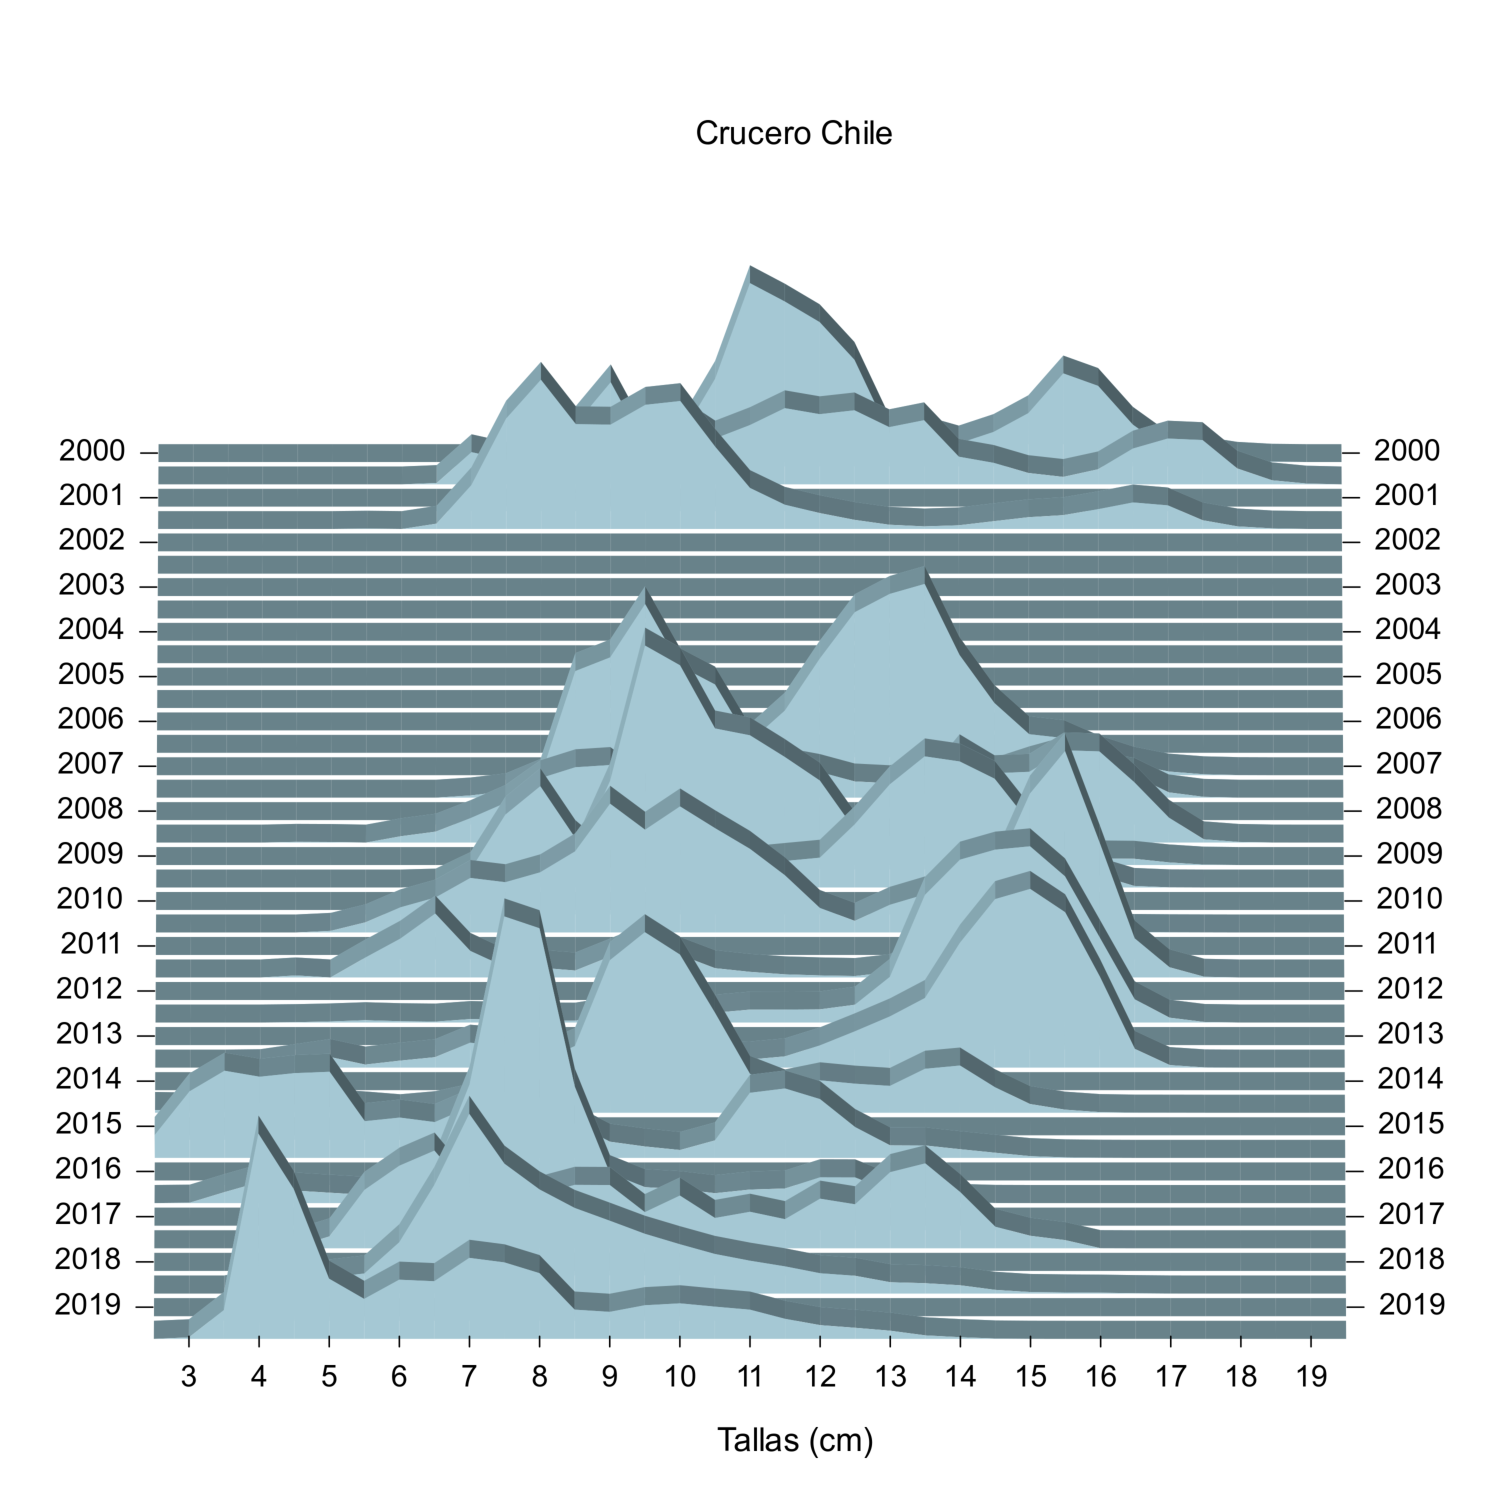
\includegraphics[width=10cm,height=8.7cm]{fig/figura01.pdf}
 \caption{Proporci\'on por tallas de la abundancia del crucero ac\'ustico en el norte de Chile (2000-2001 y 2007- 2019).}
 \label{Fig01}
\end{figure}
\vspace{0.5cm}



\vspace{0.5cm}
\begin{figure}[htb!]
 \centering
 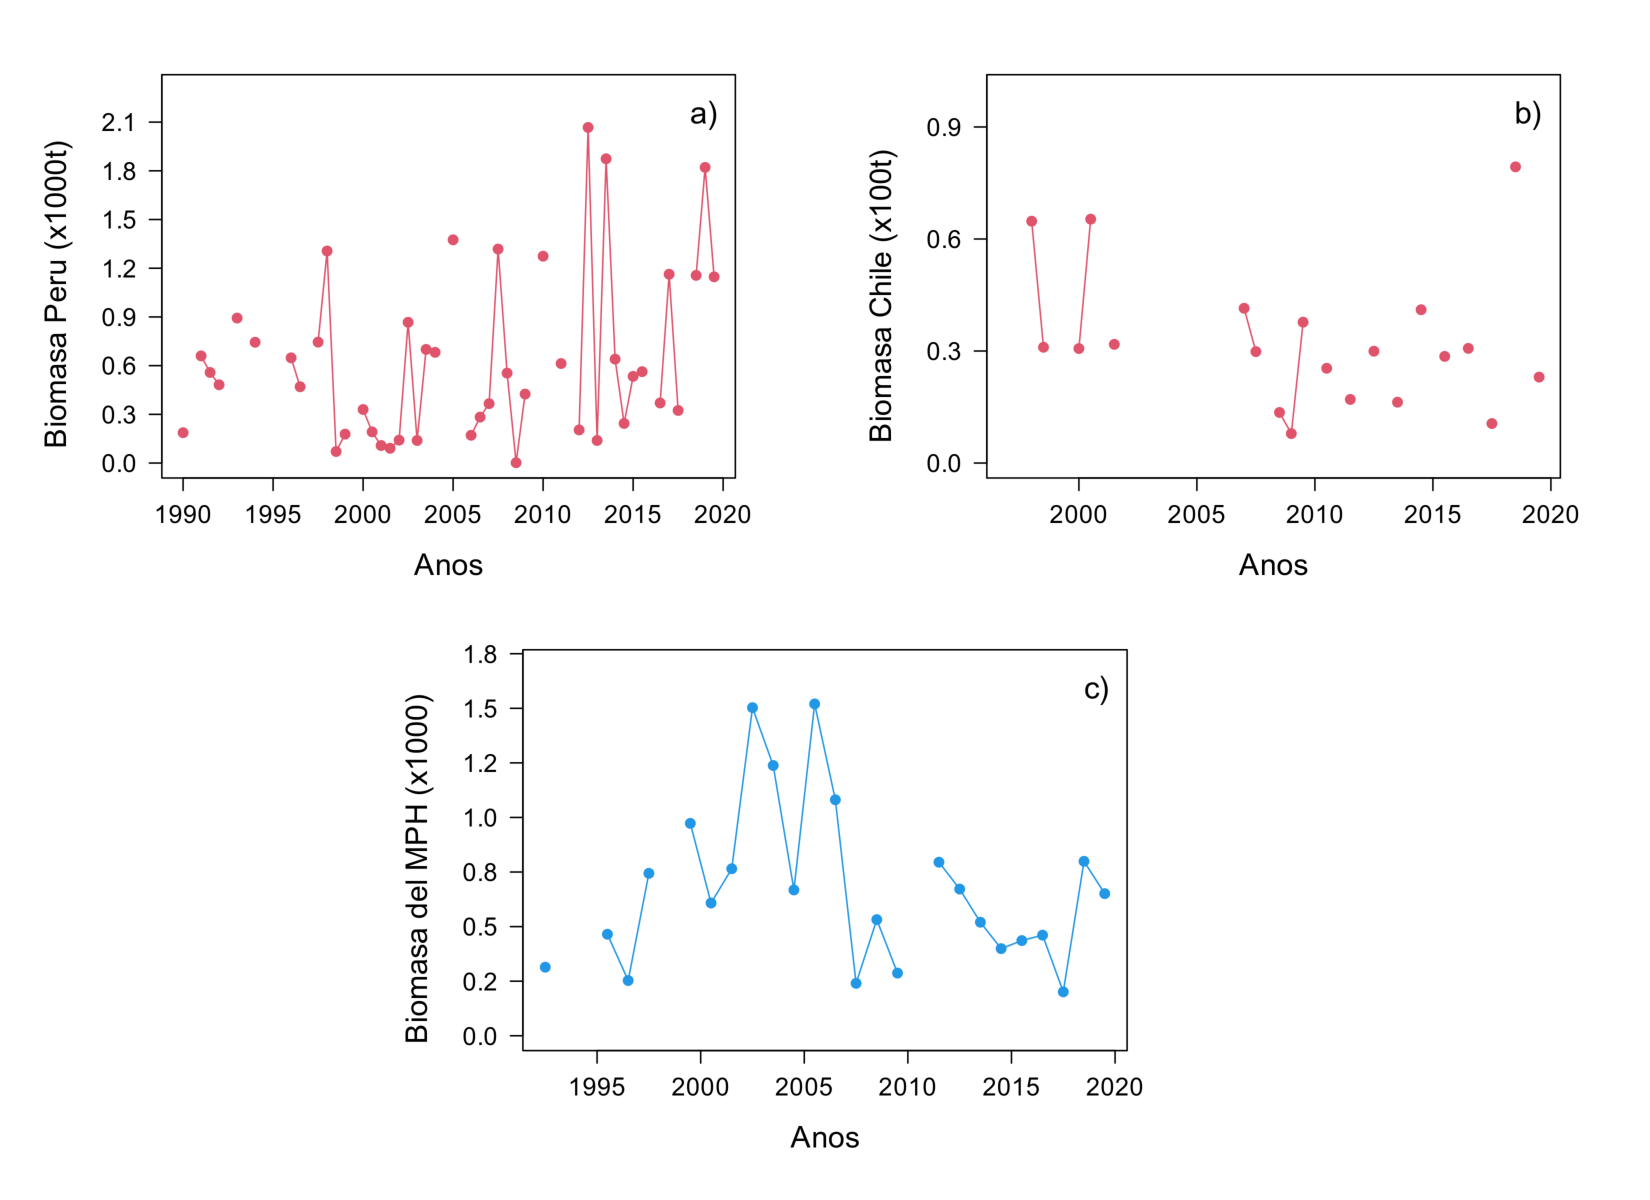
\includegraphics[width=12cm,height=11cm]{fig/figura02.pdf}
 \caption{\'Indices considerados en la evaluaci\'on del stock de anchoveta del sur de Per\'u y norte de Chile al segundo semestre del 2019, en a) la biomasa total ac\'ustica del Per\'u, b) la biomasa total ac\'ustica de Chile y c) biomasa desovante estimada a partir del MPH del norte de Chile.}
 \label{Fig02}
\end{figure}
\vspace{0.5cm}


\newpage


\subsection{Crecimiento}

Estudios recientes han reportado un r\'apido crecimiento en la fase juvenil
en algunas especies (\textit{Engraulidos}), sugiriendo que estas alcanzan
una porci\'on significativa de su longitud asint\'otica al a\~{n}o de vida (Cerna y
Plaza, 2016). En este contexto, se ejecut\'o el proyecto FIP 2009-17 que
buscaba ajustar la asignaci\'on de edad anual. Los juveniles de esta especie crecieron
a tasas muy elevadas, donde los ejemplares de 11 y 12 cm de longitud total
ten\'ian entre 4 y 5 meses de edad. Tambi\'en se pudo determinar la edad
diaria en ejemplares mayores a 12 cm de longitud total, report\'andose que
ejemplares de entre 15 y 16 cm no ten\'ian m\'as de 400 d\'ias de vida.
Posteriormente, un segundo proyecto de investigaci\'on fue ejecutado
(SUBPESCA No 4728-31 LP 11), el cual permiti\'o validar la periodicidad
diaria de formaci\'on de los micro incrementos primarios en juveniles y
adultos de esta especie en condiciones de confinamiento, lo que
ratificaba los resultados del FIP 2009-17. Finalmente, el proyecto FIP 2014-31
permiti\'o confirmar la determinaci\'on y asignaci\'on de la edad a nivel diario 
para la anchoveta en la zona norte de Chile.
Esta secuencia de proyectos involucrados en la determinaci\'on de la edad
de la anchoveta es mostrada en la \textbf{Figura \ref{Fig03}}.\\


\vspace{0.5cm}
\begin{figure}[htb!]
 \centering
 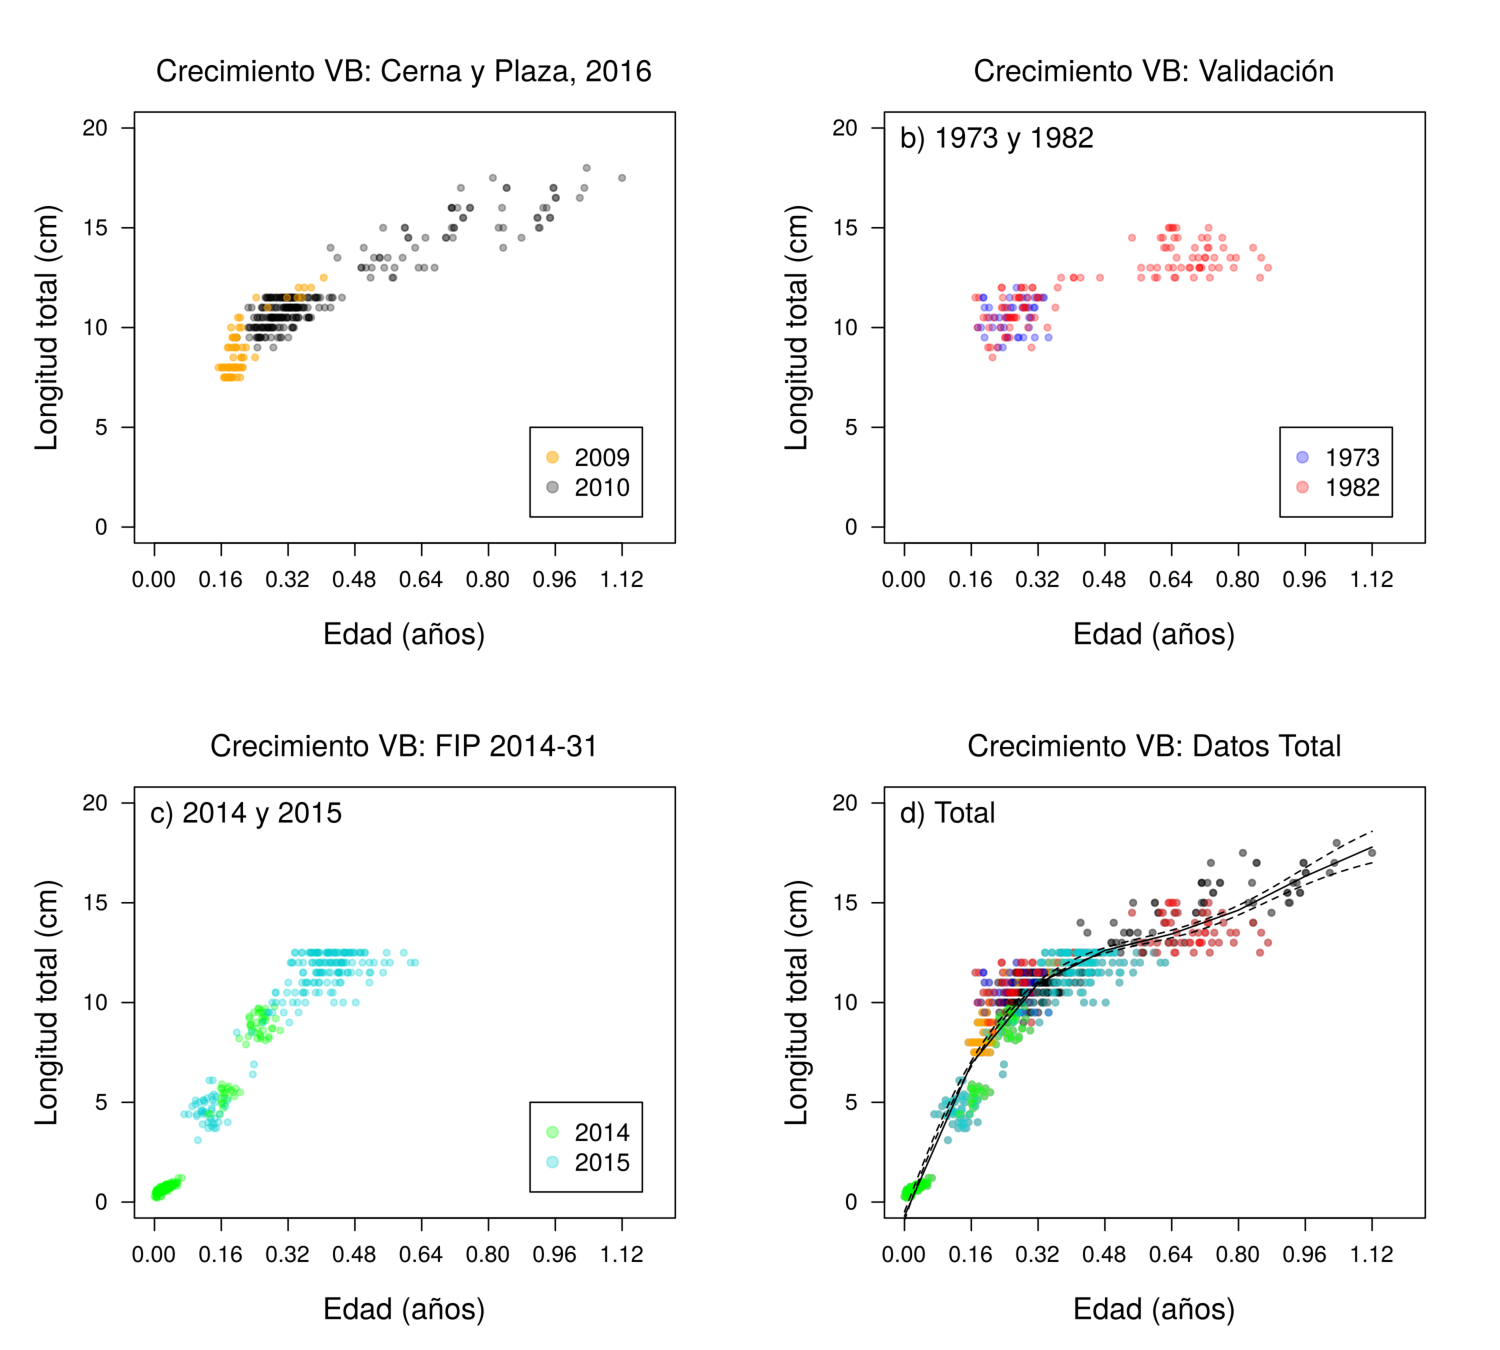
\includegraphics[width=16cm,height=12cm]{fig/figura03.pdf}
 \caption{Diferentes proyectos que dan cuenta del modelo de crecimiento de la anchoveta en la zona norte de Chile, en el panel d) se resumen todos los datos juntos de los diferentes proyectos.}
 \label{Fig03}
\end{figure}
\vspace{0.5cm}



Tambi\'en se han usado otolitos de peces capturados entre
enero y julio del 2015, a los cuales se les cont\'o el n\'umero de
incrementos desde el segundo anillo conc\'entrico que rodea el primordio
central hasta el borde del otolito. Los peces capturados correspondieron a
juveniles de entre 8.5 y 12.5 cm de longitud total con edades que fluctuaron
entre 97 y 167 d\'ias, que corresponden a peces nacidos entre julio y diciembre
del 2014 y una menor cantidad entre enero y abril (B\"ohm \textit{et al}., 2016).
Entonces, la edad de reclutamiento de la anchoveta var\'ia entre los 92
(3$^{er}$ mes) y 191 d\'ias (6$^{to}$ mes) desde la eclosi\'on. Estos resultados son
coincidentes con los reportados por Simpson y Buzeta (1967) que se\~{n}alan
dos nacimientos, uno durante el oto\~{n}o (feb-abr) y el otro en primavera
(jul-nov), con un coeficiente de crecimiento (k) de 1.6 a\~{n}o$^{-1}$ y
una longitud asint\'otica (L$_{inf}$) de 16.9 cm. Tambi\'en Saetersdal y
Valdivia (1964) reportan para el Per\'u una descendencia de verano y otra
de primavera, con la entrada de peces juveniles durante octubre-enero y
otra en marzo-junio, esta \'ultima contiene una alta proporci\'on de peces
de peque\~{n}o tama\~{n}o por debajo de los 12 cm.\\



\vspace{0.5cm}
\begin{figure}[htb!]
 \centering
 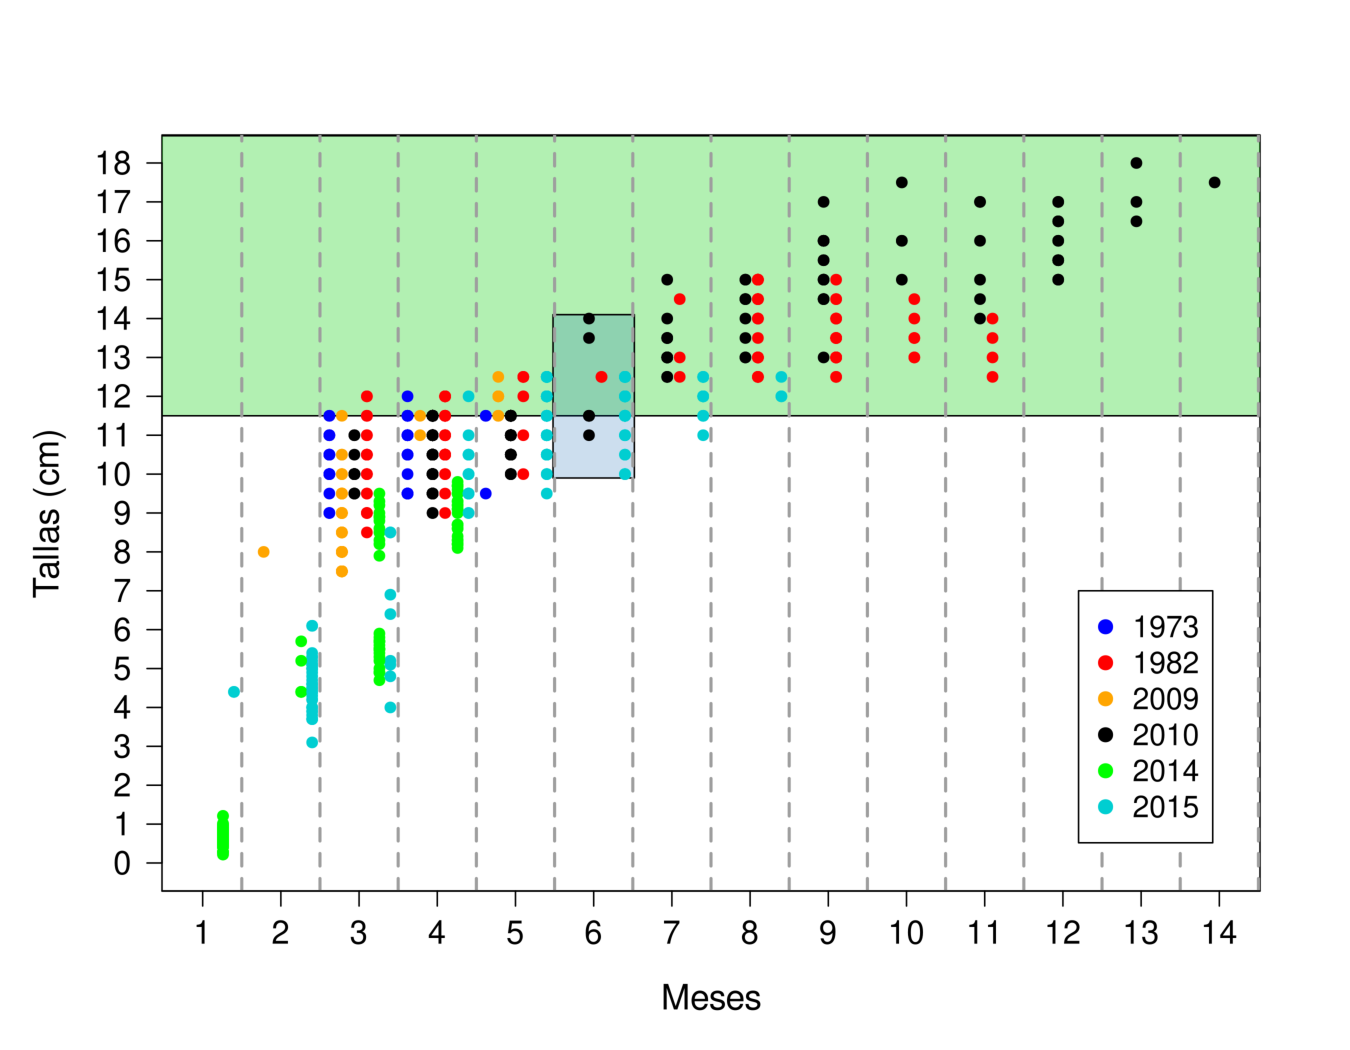
\includegraphics[width=15.5cm,height=8.5cm]{fig/figura04.pdf}
 \caption{Crecimiento de la anchoveta en una escala de tiempo mensual. La caja verde contiene los individuos sexualmente maduros que corresponde a tallas mayores e igual a 11.5 cm. Y la caja celeste contiene a los individuos de seis meses de edad con un intervalo de tallas que va desde los 10 a 14 cm de longitud total.}
 \label{Fig04}
\end{figure}
\vspace{0.5cm}



Reconfigurando los datos de microincrementos diarios (otolitos) a
una escala de tiempo mensual, esta indica que a los
tres meses de edad hay individuos de 4 y 12 cm de longitud total dependiendo del
a\~{n}o, mostrando la alta variabilidad que presenta el crecimiento de la anchoveta
en los primeros meses de vida. Estos resultados indican que habr\'ia individuos madurando
sexualmente a los 3 meses para los a\~{n}os 1973, 1982 y 2009. En cambio, para los seis
meses de edad, m\'as de la mitad de los individuos (64\%) est\'an maduros
sexualmente (\textbf{Figura \ref{Fig04}}).\\



\subsection{Mortalidad natural}


La mortalidad natural es calculada a trav\'es de diferentes modelos
bio-anal\'ogicos existentes en la literatura seg\'un los par\'ametros de
crecimiento anteriormente se\~{n}alados. Estos
modelos entregan un valor superior a dos (\textbf{Tabla \ref{Tab2}}),
para lo cual en el modelo de evaluaci\'on de stock se utiliza un valor de $M=1.1$ 
(semestre$^{-1}$) para la tasa de mortalidad natural ($M$), valor usado como constante para
todas las edades y semestres.\\

\vspace{0.5cm}
\begin{table}[htb!]
 \caption{M\'etodos emp\'iricos para estimar la mortalidad natural.}
 \label{Tab2}
 \vspace{0.01cm}
 \centering
 \vspace{0.2cm}
 \small
 \begin{tabular}{lccc}
 \noalign{\vskip 0.1cm}
 \cline{2-4} & \multicolumn{3}{c}{Edad te\'orica m\'axima} \\
 \hline
 \noalign{\vskip 0.1cm}
  M\'etodo  & \--- & 1 & 2 \\
 \hline
 \noalign{\vskip 0.2cm}
 Rikhter y Efanov (1976) & 2.78 & \--- & \--- \\
 Pauly (1980) & 1.74 & \--- & \--- \\
 Taylor (1958, 1960) & \--- & 2.16 & 1.99 \\
 Hoening (1983) & \--- & 2.16 & 2.14 \\
 Alverson y Carney (1975) & \--- & 2.33 & 2.28 \\
 Alagaraja (1984) & \--- & 2.33 & 2.30 \\
 Hewitt y Hoening (2005) & \--- & 2.14 & 2.11 \\
 \noalign{\vskip 0.1cm}
 \hline
 \noalign{\vskip 0.1cm}
 \textbf{Promedio} & \textbf{2.26} & \textbf{2.22} & \textbf{2.17} \\
 \noalign{\vskip 0.1cm}
 \hline
 \noalign{\vskip 0.2cm}
 \multicolumn{1}{l}{(1) $T_{max}=t_{0}+\frac{3}{k}$}
 \end{tabular}
\end{table}
\vspace{0.5cm}



\subsection{Reclutamiento}


Observaciones, \textit{in situ}, hist\'oricamente han mostrado que el ingreso de 
reclutas ocurre desde octubre hasta marzo, sin embargo, durante los \'ultimos a\~{n}os
se ha detectado una mayor presencia de reclutas desde abril hasta agosto (B\"ohm \textit{et al}., 2016). Por otro lado, la distribuci\'on de longitudes observada por el crucero hidroac\'ustico
estim\'o un 73\% de reclutas, distribuy\'endose los ejemplares entre 2.5 y 16 cm
(Leiva \textit{et al}., 2016), con una alta presencia de individuos de 2.5 y 5 cm asociados a la
franja costera. Durante la fase c\'alida del evento ENOS se observa un
alto porcentaje de ejemplares menores a los 12 cm, alcanzando un 70\% la
presencia de reclutas en las capturas de la flota industrial (Bertrand
\textit{et al}., 2004; B\"ohm \textit{et al}., 2016). Adem\'as, durante el
\'ultimo tiempo se ha observado una disminuci\'on de las tallas medias en la
flota industrial, donde la falta de ejemplares adultos ha estado ausente
en los \'ultimos a\~{n}os. La distribuci\'on de longitudes en las capturas de la
flota industrial chilena muestra un patr\'on unimodal con una talla media
de 14.7, 14.1, 13.0, 12.1, 12.6, 13.2 y 11.4 cm en el 2013, 2014,
2015, 2016, 2017, 2018 y 2019 respectivamente.\\


El modelo de evaluaci\'on de stock de la anchoveta del sur de Per\'u y norte de Chile
tiene una escala de tiempo semestral en a\~{n}o calendario, y al inicio de cada
semestre se produce la entrada de los reclutamientos como desviaciones desde R$_{0}$.
Estas estimaciones muestran que los reclutamientos registrados durante el segundo
semestre han sido en promedio de mayor intensidad respecto de los registrados en el
primer semestre (\textbf{Figura \ref{Fig05}}), y esto se deber\'ia principalmente a que
el reclutamiento del segundo semestre es el que soporta las capturas del primer
semestre (debido al r\'apido crecimiento, ver \textbf{Figura \ref{Fig04}}), donde se registra
la mayor proporci\'on de la captura del a\~{n}o. Desde mediados del 2008 hasta el 2015 los
reclutamientos semestrales han alcanzado un valor medio de 230 ($\pm$143) millones de
individuos. En segundo semestre del 2015 se registr\'o el valor m\'as bajo de la serie.\\


\vspace{0.5cm}
\begin{figure}[htb!]
 \centering
 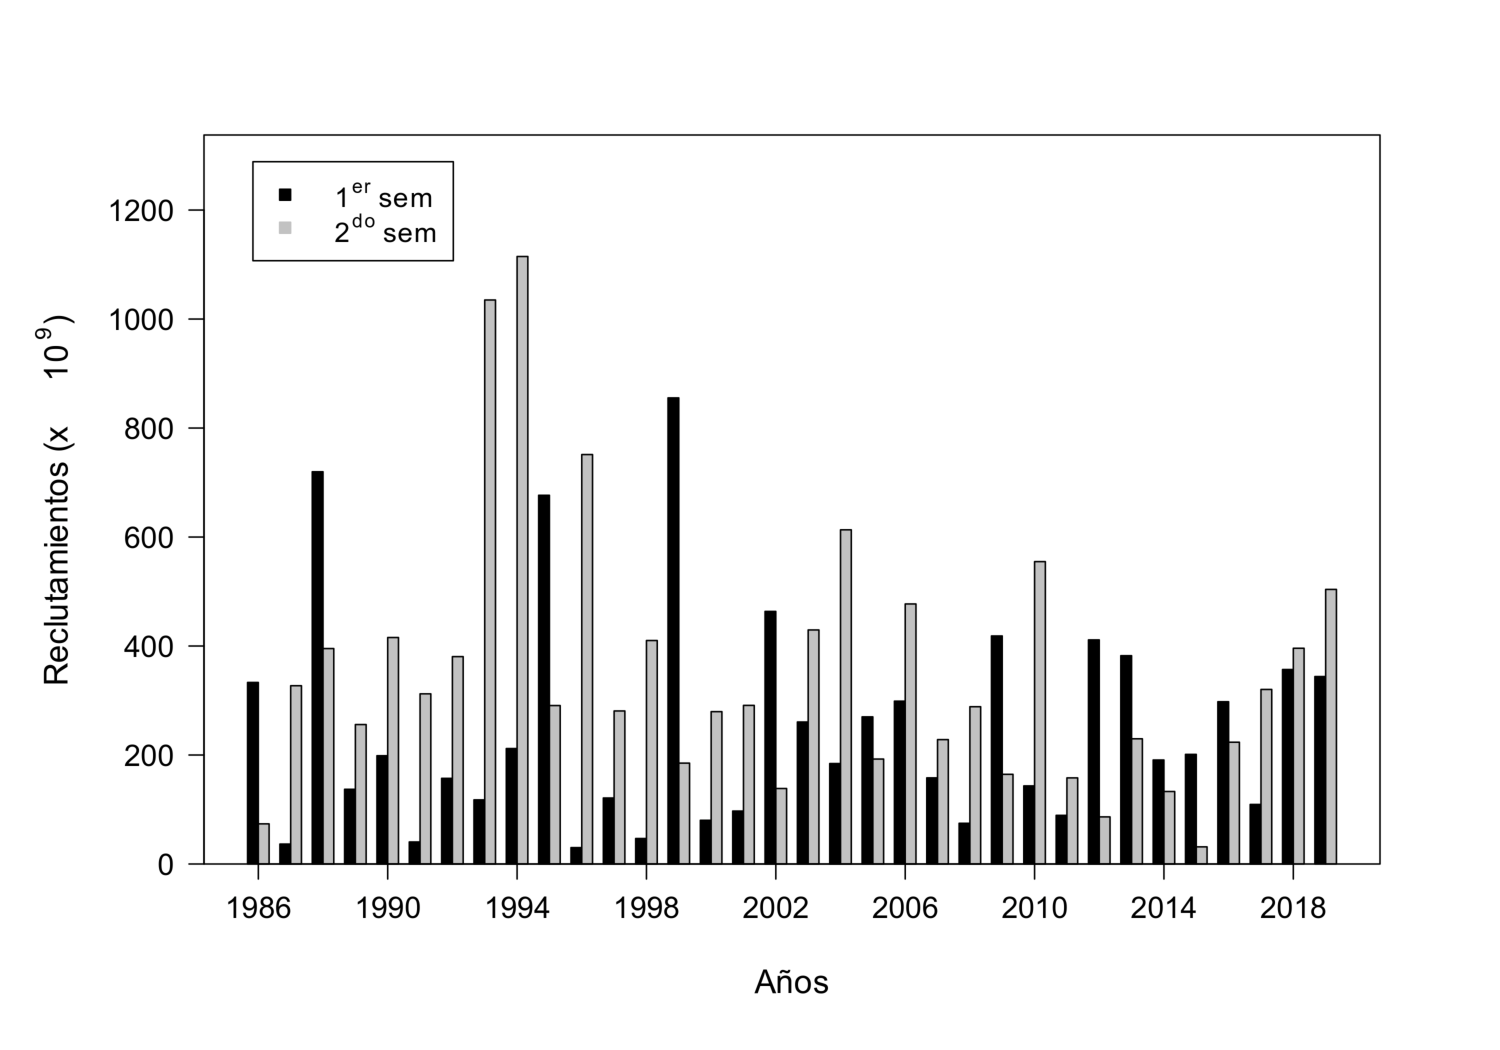
\includegraphics[width=12cm,height=8cm]{fig/figura05.pdf}
 \caption{Reclutamientos semestrales estimados por el modelo de evaluaci\'on para la 
 anchoveta del sur de Per\'u y norte de Chile.}
 \label{Fig05}
\end{figure}
\vspace{0.5cm}


Los desv\'ios de los reclutamientos semestrales estimados por el modelo de evaluaci\'on
de stock indican, respecto de su tendencia de largo plazo, anomal\'ias negativas desde
el 2008 hasta el primer semestre del 2017, y en el segundo semestre del 2017 esta tendencia
se revierte (anomal\'ia positiva), con anomal\'ias de 0.08, 0.21, 0.36, 053 y 0.72 para el
2017.5, 2018.0, 2018.5, 2019.0 y 2019.5, respectivamente. Sin embargo, las estimaciones
semestrales indican que durante el segundo semestre del 2015 se registr\'o el valor m\'as bajo
durante los \'ultimos veinte a\~{n}os (\textbf{Figura \ref{Fig06}}). Dada esta tendencia negativa
en los reclutamientos en el largo plazo durante los a\~{n}os 2008-2017 (\textbf{Figura \ref{Fig06}}),
la biomasa de este recurso ha registrado una importante disminuci\'on en comparaci\'on con los
valores estimados antes del a\~{n}o 2000. Sin embargo, en los \'ultimos cruceros ac\'usticos
realizados en el norte de Chile han registrado altos valores de biomasas total, con un alto
porcentaje correspondiente a la fracci\'on menor a los 11.5 cm
(biomasa de reclutas) de longitud total, por sobre el promedio hist\'orico. El reclutamiento del 2016
es uno de los mayores registrados en la \'ultima d\'ecada, superior en un 24\% al reclutamiento observado en el 2015, y muy similar al observado en el 2014. Es decir, durante los a\~{n}os 2015-16-17 se han registrado un valor medio de 241 ($\pm$) 28 mil toneladas de biomasa de reclutas. Aunque,
en el segundo semestre del 2017 este valor alcanz\'o las 41 mil toneladas (Leiva \textit{et al}., 2018). Sin embargo, a finales del 2018 se registr\'o un valor de 596 mil toneladas de biomasa de 
reclutas, valor m\'as alto de la serie historia desde que se hace el crucero ac\'ustico (1996) en el norte de Chile.\\


\vspace{0.5cm}
\begin{figure}[htb!]
 \centering
 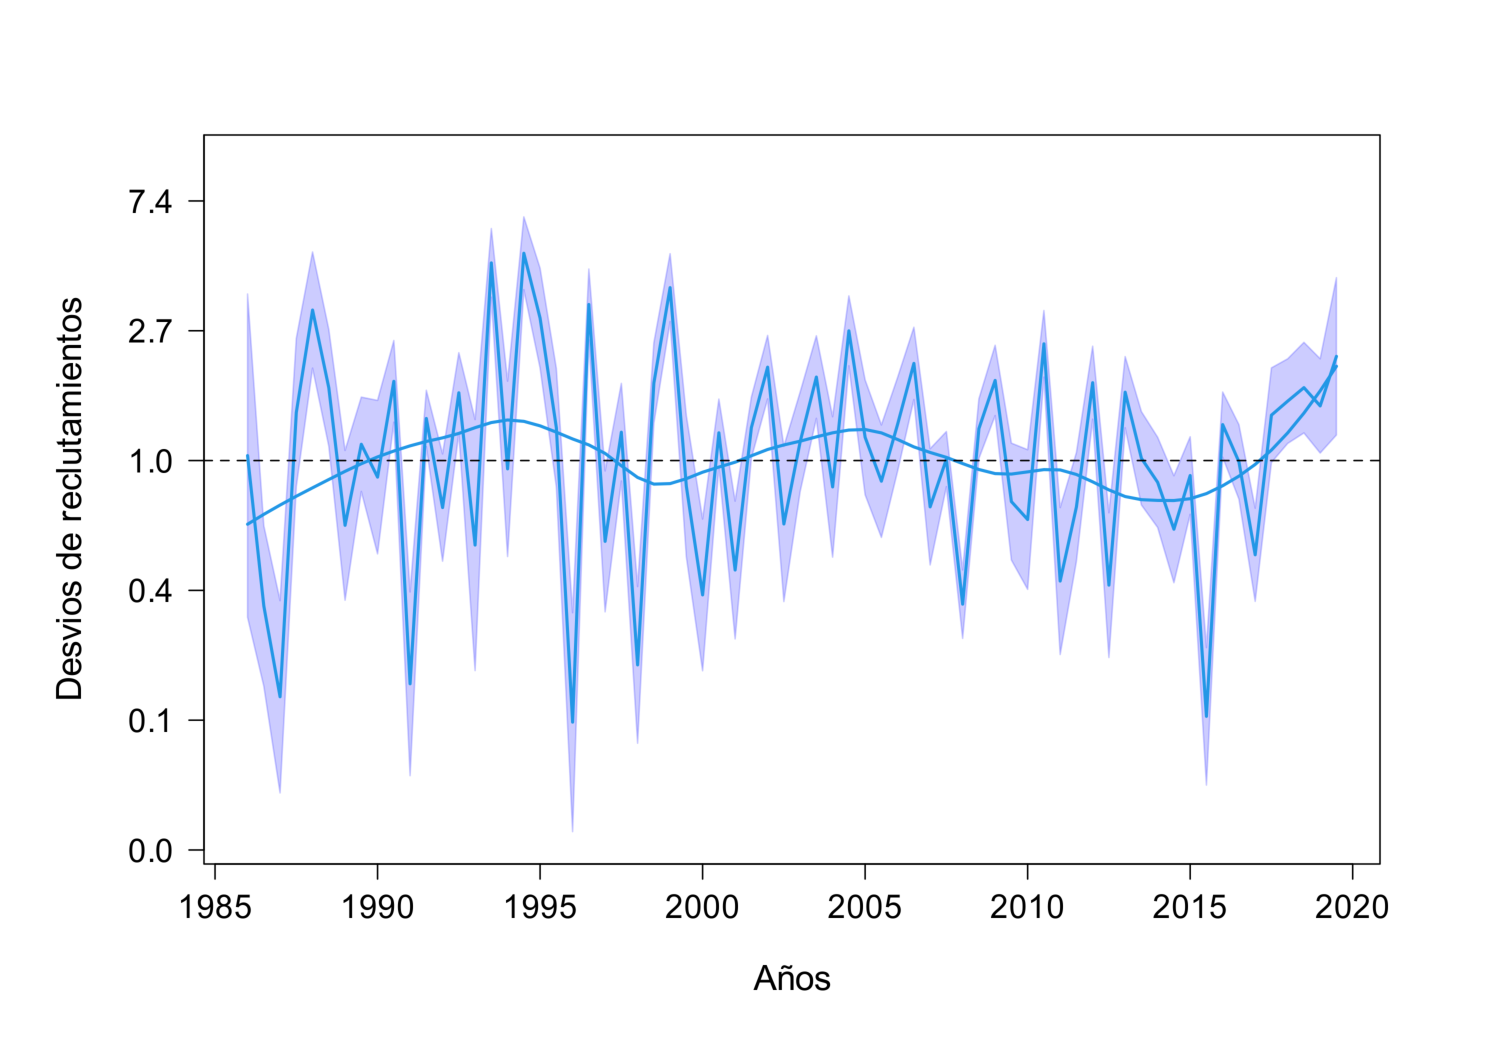
\includegraphics[width=12cm,height=8cm]{fig/figura06.pdf}
 \caption{Desvios de los reclutamientos estimados por el modelo de evaluaci\'on para la 
 anchoveta del sur de Per\'u y norte de Chile.}
 \label{Fig06}
\end{figure}
\vspace{0.5cm}



Esta contradicci\'on entre los desv\'ios de los reclutamiento estimados por el modelo de evaluaci\'on
y las observaciones directas sobre la biomasa total y la de reclutas del sotck de anchoveta en el norte
de Chile, se ve acentuada con las bajas capturas que se registraron durante este periodo, durante el segundo semestre del 2016 la captura total fue de 101 mil toneladas y en el segundo semestre
del 2017 la captura total fue de 178 mil toneladas. Las bajas capturas durante este periodo se debe 
a la alta presencia de individuos juveniles de menor tamaño que son evitados por la flota industrial,
producto del enmallamiento de las redes de cerco y los bajos niveles de rendimiento para las plantas de
proceso. Entonces, durante este periodo la alta presencia de biomasa de reclutas no se traducen
posteriormente (6 meses) en altas capturas, lo que podr\'ia deberse a diversos procesos f\'isicos, qu\'imicos y biol\'ogicos producto del calentamiento global que afectan a los ecosistemas marinos. \\


\subsection{An\'alisis retrospectivo}

Una manera de probar la capacidad del modelo de evaluaci\'on y de sus resultados a la
ausencia o exclusi\'on de series de informaci\'on es el an\'alisis retrospectivo. Este
an\'alisis mide la coherencia entre estimaciones sucesivas de un mismo par\'ametro a
medida que se eliminan datos en forma secuencial. En muchas aplicaciones se ha visto
que la varianza estad\'istica en la estimaci\'on de abundancia (o mortalidad por pesca)
tiende a disminuir con el transcurso del tiempo, y las estimaciones del \'ultimo a\~{n}o
(utilizadas en el manejo pesquero) son poco confiables (Sinclair et al., 1991; Mohn, 1993;
Parma, 1993). Estos errores retrospectivos pueden deberse a muchas razones, desde sesgo
en los datos de captura, hasta diferentes tipos de espec\'ificaciones  err\'oneas en el
modelo, como par\'ametros que se asumen que son constantes en el an\'alisis pero que en
realidad cambian, así como supuestos erroneos sobre la vulnerabilidad relativa de ciertas
clases de edad.\\


\vspace{0.5cm}
\begin{figure}[htb!]
 \centering
 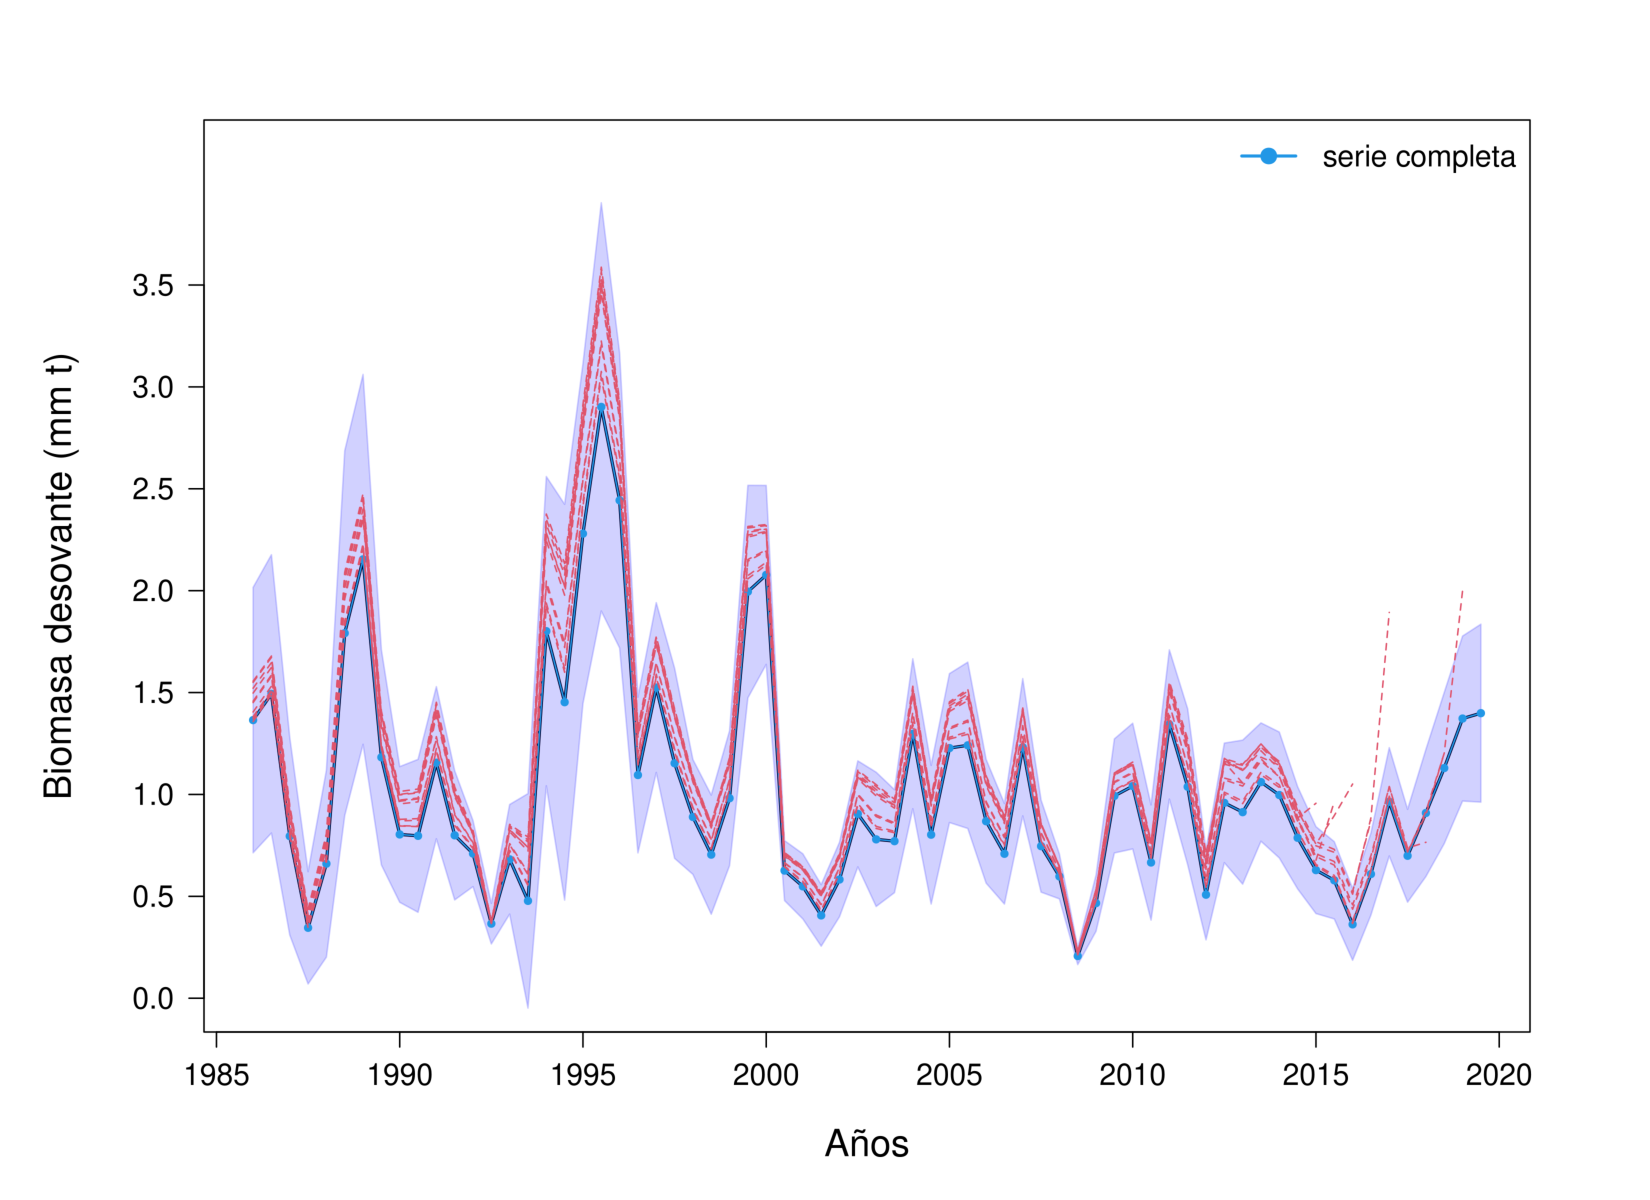
\includegraphics[width=15cm,height=9cm]{fig/figura07.pdf}
 \caption{An\'alisis retrospectivo para la biomasa desovante de la anchoveta del sur de Per\'u y norte de Chile. La sombra en azul representa el intervalo de confianza al 95\% para la serie
 completa y la l\'inea azul representa la estimaci\'on media para la serie completa.
 Las \'ineas segmentadas en rojo representan las biomasas desovantes estimadas al descuento de 
 informaci\'on.}
 \label{Fig07}
\end{figure}
\vspace{0.5cm}



\vspace{0.5cm}
\begin{figure}[htb!]
 \centering
 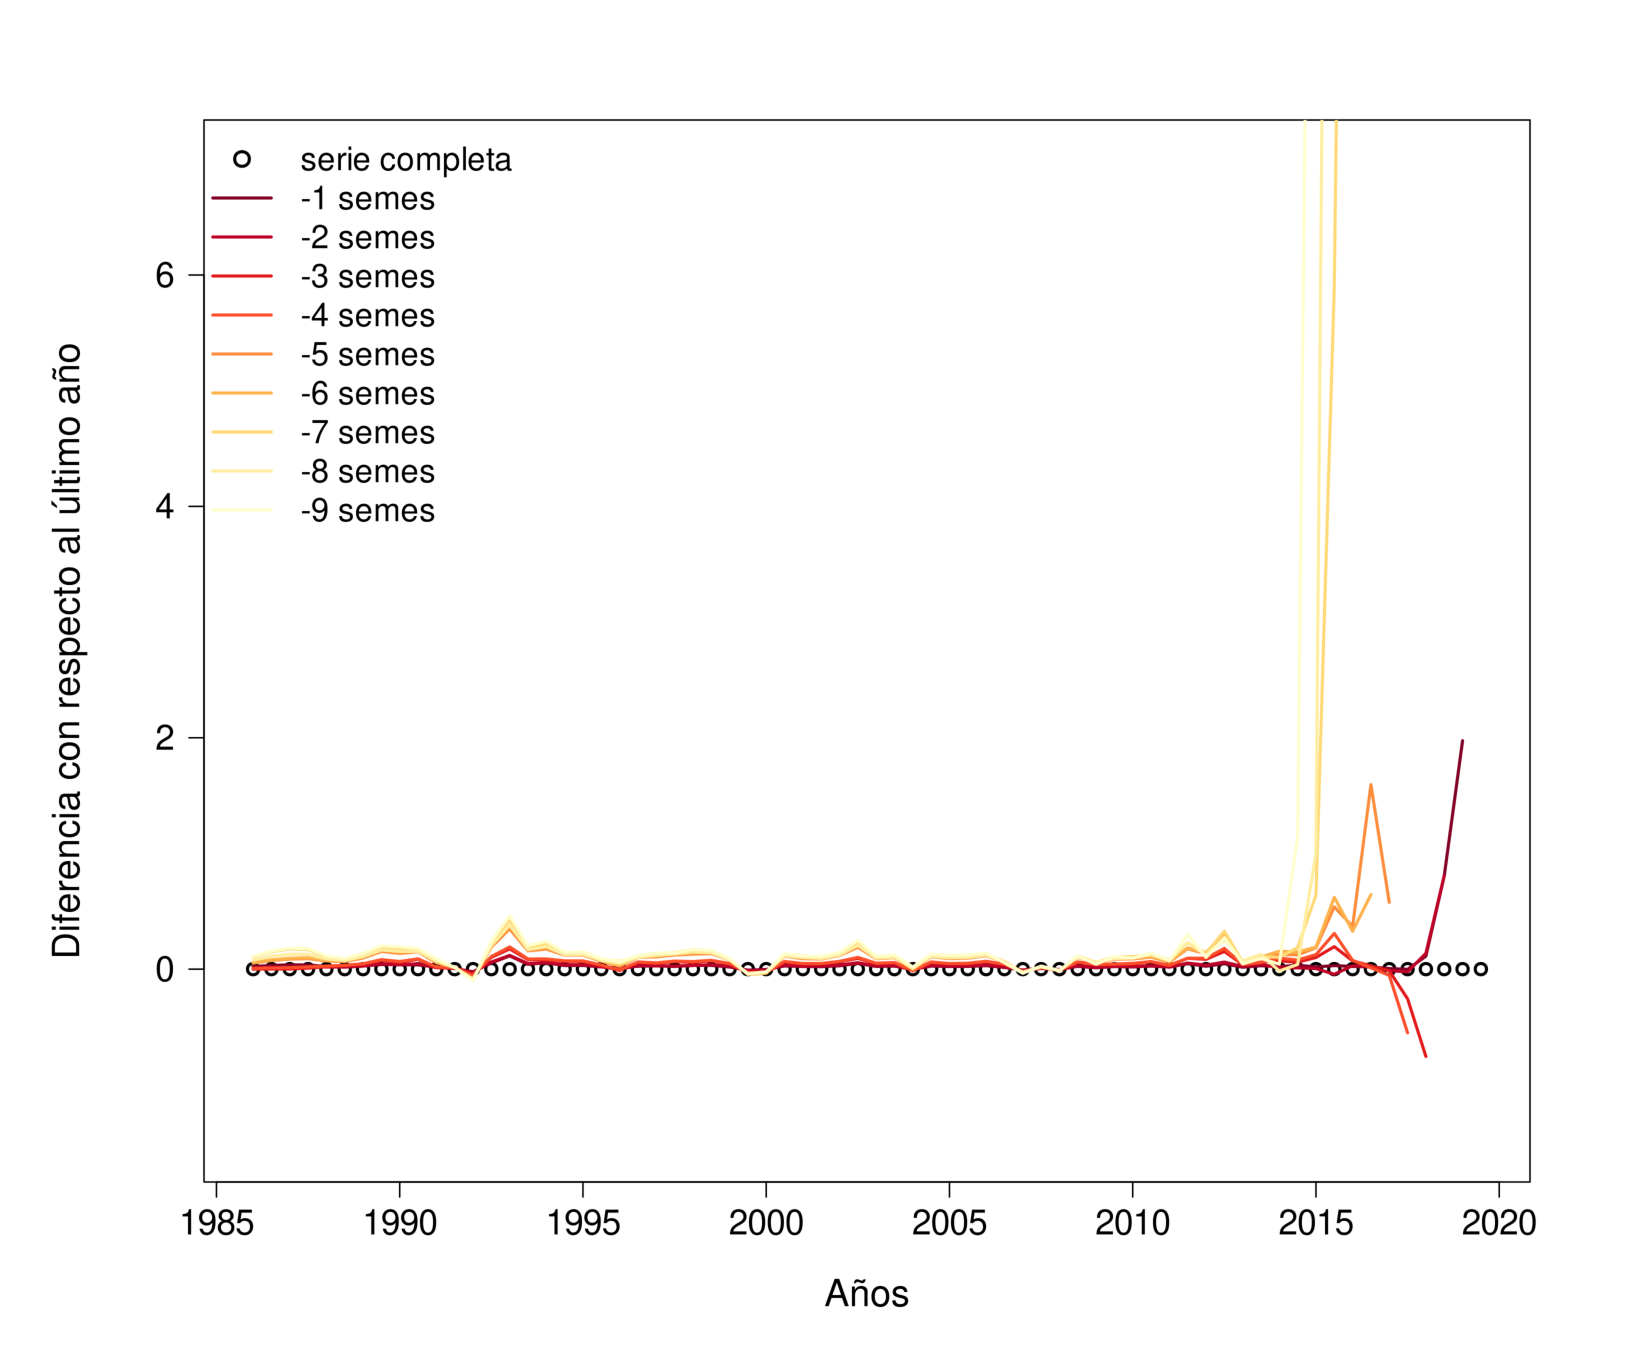
\includegraphics[width=15cm,height=9cm]{fig/figura08.pdf}
 \caption{Patr\'on retrospectivo para los \'ultimos nueve semestres de \textit{rho} de Mohn
 para la serie de los reclutamientos como una diferencia del \'ultimo a\~{n}o de la evaluaci\'on
 de la anchoveta del sur de Per\'u y norte de Chile.}
 \label{Fig08}
\end{figure}
\vspace{0.5cm}



En la \textbf{Figura \ref{Fig07}} se muestra el an\'alisis retrospectivo para la biomasa desovante
de la anchoveta del sur de Per\'u y norte de Chile, la cual se llev\'o a cabo mediante la eliminaci\'on
sistem\'atica de los \'ultimos cinco a\~{n}os de la serie de datos, secuencialmente por semestre.
Los resultados muestran un patr\'on retrospectivo a sobreestimar la biomasa desovante al descuento del primer, quinto, sexto, s\'eptimo y octavo semestre, es decir, hace un semestre (2019.0), dos a\~{n}os
y medio atr\'as (2017.0), tres a\~{n}os (2016.5), tres a\~{n}os y medio (2015.0) y cuatro a\~{n}os
atr\'as (2014.5). Las diferencias en los niveles de biomasa desovante resultan ser muy marginales para el resto de los descuentos, incluso se tiende a subestimar la biomasa desvoante en el primer semestre
del 2017.\\


El an\'alsisis retrospectivo puede ser visualizado tambi\'en como la suma de las diferencias
relativas entre un par\'ametro estimado de la evaluaci\'on con todos los datos, y el mismo
par\'ametro estimado con respecto a una serie de tiempo reducida. Este estad\'istico es
conocido como \textit{rho} de Mohn (1999), y su c\'alculo ser\'a cero cuando la evaluaci\'on
descontada sea igual con la evaluaci\'on con todos los datos, o cuando las diferencias
entre la evaluaci\'on descontada y la de la evaluaci\'on con todos los datos son balanceados
por las diferencias postivias y negativas. El estad\'istico de \textit{rho} de Mohn ser\'a
grande, si es positivo o negativo, cuando hay un consistente patr\'on de cambio en la
evaluaci\'on descontada relativo a la evaluaci\'on con todos los datos. En la \textbf{Figura 
\ref{Fig08}} se muestra el estad\'istico de \textit{rho} de Mohn para los reclutamientos, el
cu\'al muestra diferencias inferiores a 0.5 para los dos \'ultimos a\~{n}os. Sin embargo,
se observ\'o un valor de \textbf{1.97} para el primer semestre del 2019 y un valor de \textbf{0.81}
para el segundo semestre del 2018. Luego, las diferencias cambia a valores negativos de 0.75 y
0.55 para el primer semestre del 2018 y el segundo semestre del 2017, respectivamente.\\




\subsection{Estatus}

El estado de explotaci\'on del stock de anchoveta del sur de Per\'u y norte
de Chile fue evaluado conforme al est\'andar adoptado por el Comit\'e
Cient\'ifico T\'ecnicos (CCT) y es sustentado en la estimaci\'on de los Puntos
Biol\'ogicos de Referencia (PBR) especie-espec\'ificos (Pay\'a et al., 2014). Los proxies al
Rendimiento M\'aximo Sostenido (RMS) son: i) la biomasa al rendimiento
m\'aximo sostenido (B$_{RMS}$) es igual al 50\% de la biomasa desovante
virginal (BD$_{0}$) y ii) la mortalidad por pesca al RMS (F$_{RMS}$)
es aquella mortalidad por pesca que en el largo plazo produce el 55\% de
la biomasa desovante por recluta igual a F55\%BDPR (Beverton y Holt,
1957). Es decir, el valor de mortalidad por pesca objetivo al segundo
semestre del 2019 es de 0.86 semestre$^{-1}$, con una alta variabilidad en
el tiempo (d\'ecada del 90) con un valor medio de 1.13 y un coeficiente de 
variaci\'on del 37\%, influenciada particularmente por el patr\'on de 
explotaci\'on. Y la biomasa desovante virginal se ha estimado en 1.28 millones
de tonaledas ($\pm$73 mil toneladas), entonces el proxy de la biomasa desovante al
rendimiento m\'aximo sostenible (50\%BD$_{0}$) es cercano a las 640 mil tonealdas.\\


Considerando los PBR menacionados anteriormente, la mortalidad por pesca muestra un
patr\'on fluctuante desde mediados de 1992, en varios periodos donde se registran
valores por sobre el F$_{RMS}$ y otros periodos por debajo del
F$_{RMS}$. Sin embargo, desde el 2010 a la fecha los valores se ubican
por debajo del F$_{RMS}$, generando con esto una condici\'on sin
sobrepesca (\textbf{Figura \ref{Fig09}}), y al \'ultimo semestre de la
evaluaci\'on la mortalidad por pesca se encuentra un 86\% por debajo del
objetivo de manejo. De igual manera, los resultados indican que la
reducci\'on de la biomasa ocurrida a mediados del 2008 y en 2016 llevaron
a la poblaci\'on a valores por debajo de la biomasa al RMS, generando con
ello un estado de sobreexplotaci\'on. Sin embargo, la reducci\'on de la
mortalidad por pesca observada durante los \'ultimos a\~{n}os y la alta
variabilidad observados en los reclutamientos han llevado a la poblaci\'on
a niveles por encima del punto biol\'ogico de referencia objetivo de manejo,
y esto se traduce que desde mediados del 2016 a la fecha ha variado en torno a
un 1.57 ($\pm$ 0.47). Al \'ultimo semestre de la evaluaci\'on la biomasa
desovante se encuentra un 118\% superior al objetivo de manejo, y dado
los niveles de incertidumbre, existe una nula probabilidad de que la
BD$_{2019.5}$ $<$ BD$_{RMS}$ (\textbf{Figura \ref{Fig09}}),
generando con ello un estado de subexplotaci\'on en biomasa desovante.\\


\vspace{0.5cm}
\begin{figure}[htb!]
 \centering
 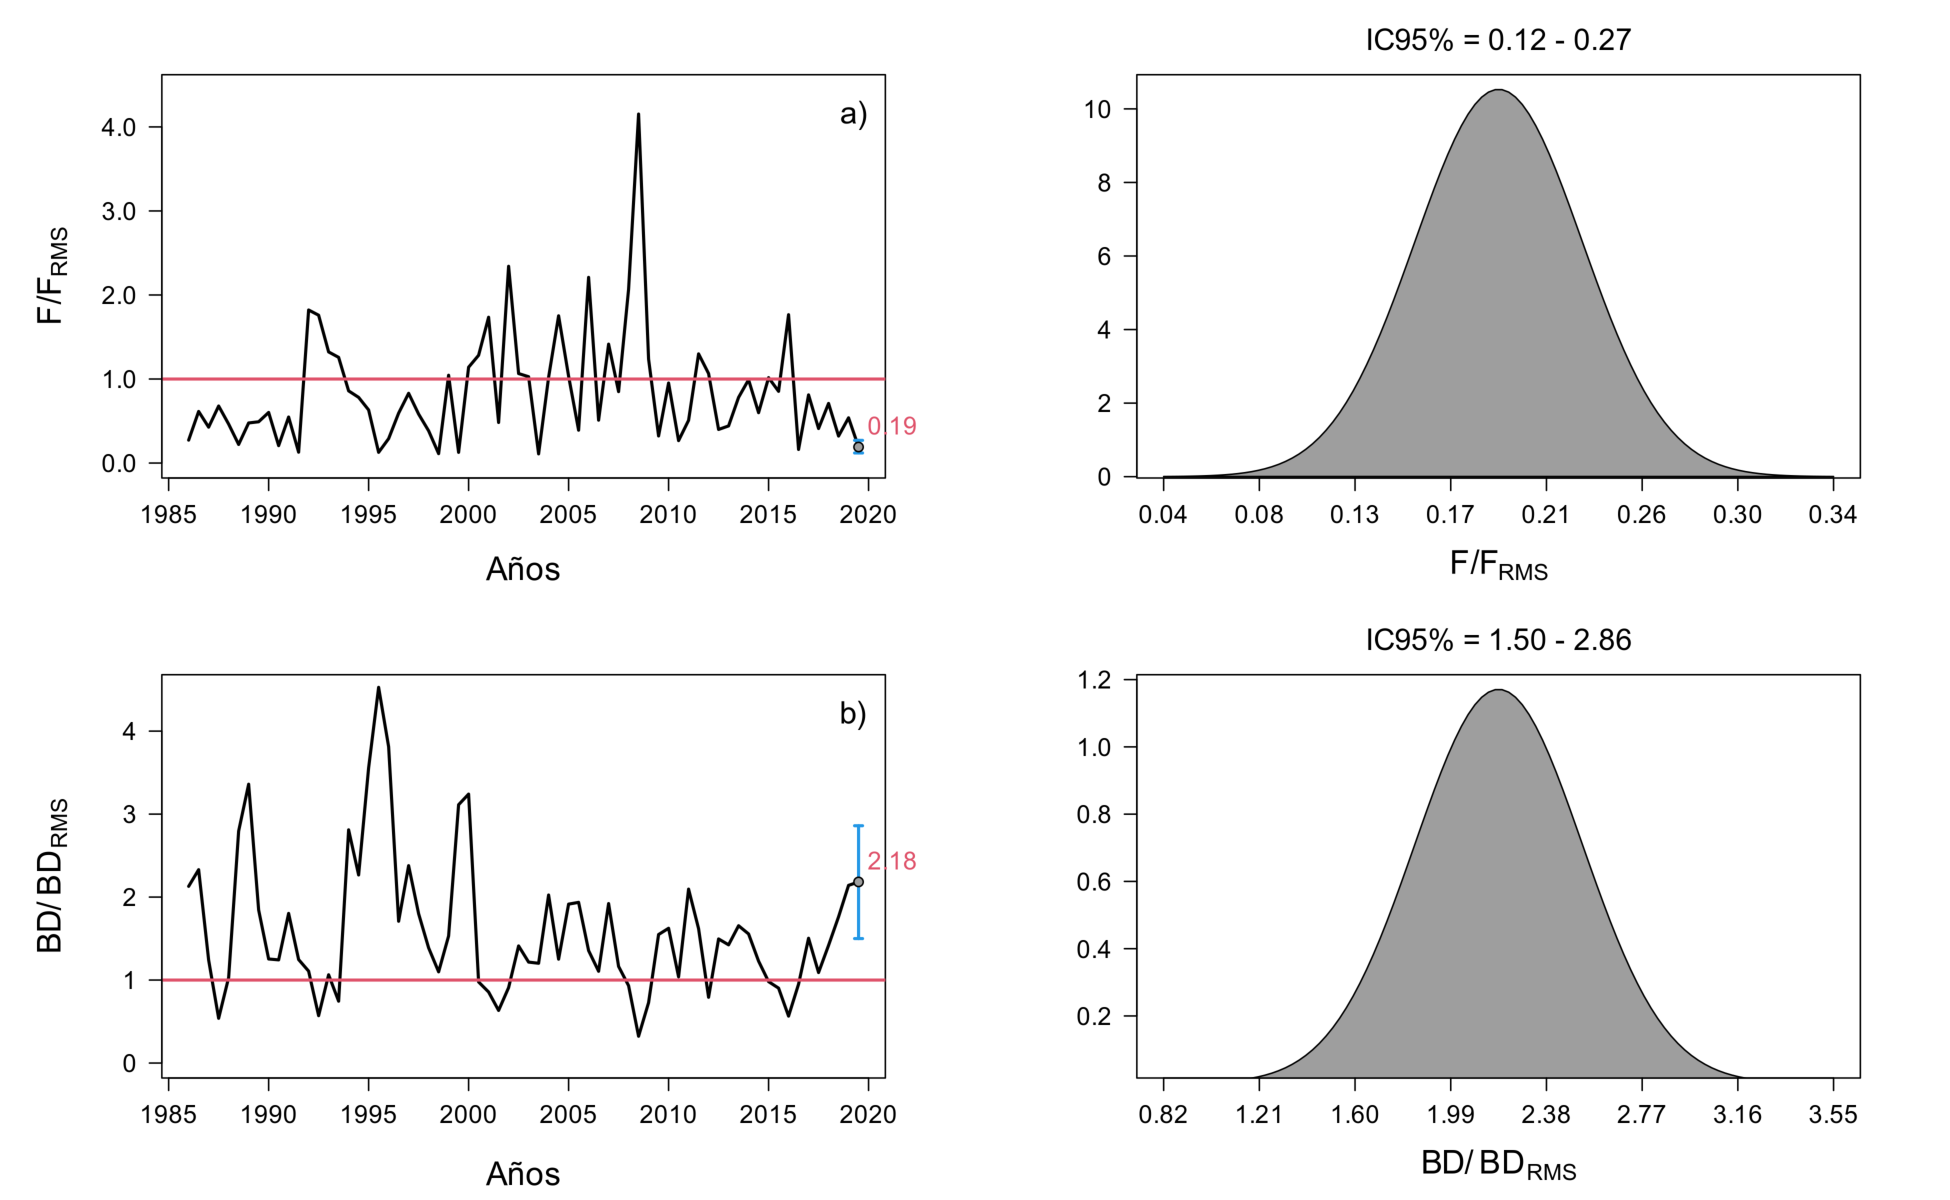
\includegraphics[width=15cm,height=10cm]{fig/figura09.pdf}
 \caption{Serie temporal de la raz\'on de la mortalidad por pesca respecto a su referente asociado al RMS y la incertidumbre al \'ultimo semestre de la evaluaci\'on en el planel superior (a) y la serie temporal de la raz\'on de la biomasa desovante respecto a su referente asociado al RMS y la incertidumbre al \'ultimo semestre de la evaluaci\'on en el panel inferior (b) para la anchoveta del sur de Per\'u y norte de Chile. La l\'inea roja representa el objetivo de manejo referido al RMS.}
 \label{Fig09}
\end{figure}
\vspace{0.5cm}



\subsection{Captura Biol\'ogicamente Aceptable (CBA)}

De acuerdo al ciclo de manejo hist\'orico de esta pesquer\'ia, la
recomendaci\'on de CBA comienza con el c\'alculo de la CBA inicial que
permite al CCT-PP, en octubre de cada a\~{n}o, establecer el estatus y
recomendar el rango de CBA para el a\~{n}o siguiente. En el mes de
diciembre, el crucero de evaluaci\'on hidroac\'ustico permite estimar la
abundancia y biomasa total en el norte de Chile (fines de a\~{n}o) y sur de Per\'u
(primavera y verano), esta informaci\'on junto a datos provenientes de la
pesquer\'ia de Chile y Per\'u y la estimaci\'on de la biomasa desovante
(oto\~{n}o-primavera) a partir del m\'etodo de producci\'on diaria de huevos,
es utilizada para la actualizaci\'on de la CBA (\textbf{Tabla \ref{Tab3}}).\\



\vspace{0.5cm}
\begin{table}[htb!]
 \caption{Informaci\'on relevante para el c\'alculo de CBA 2021 en cada una de las etapas de estimaci\'on.}
 \label{Tab3}
 \centering
 \small
 \begin{tabular}{lcc}
 \hline\noalign{\vskip 0.1cm}
 Datos de entrada & CBA inicial & CBA actualizada \\
 \hline\noalign{\vskip 0.1cm}
 Desembarques Chile & 1986.0 - 2019.5 & 1986.0 - 2020.5 \\
 Desembarques Per\'u & 1986.0 - 2019.5 & 1986.0 - 2020.5 \\
 Descarte Chile & 2017 - 2019.5 & 2017 - 2019.5 \\
 Biomasa ac\'ustica Per\'u & 1990-2019.5 & 1990 - 2020.5 \\
 Biomasa ac\'ustica Chile & 1997-2002, 2007-2019.5 & 1997-2002, 2007-2020.5 \\
 Biomasa desovante Chile (MPDH) & 1992-2019 & 1992-2020.5 \\
 Composici\'on de tallas flota Per\'u & 1986 -2019.5 & 1986 - 2020.5 \\
 Composici\'on de tallas flota Chile & 1986 - 2019.5 & 1986 - 2020.5 \\
 Composici\'on de tallas crucero Chile & 2000-2002 y 2007-2019 & 2000-2002 y 2007-2020 \\
 Pesos medios a la talla Chile & 2001 - 2019.5 & 2001 - 2020.5 \\
Proyecci\'on del reclutamiento & 4 semestres & 2 semestres \\
 \hline
 \end{tabular}
\end{table}
\vspace{0.5cm}



La \textbf{Tabla \ref{Tab4}} muestra las CBA recomendadas por el CCT-PP
en las distintas etapas de establecimiento de cuotas, desembarques
registrados y sus diferencias, entre el 2015 y 2020. Entre el 2016 y
2019 se mantuvo una CBA statu quo en 760 mil toneladas, en ambos hitos
de manejo (CBA inicial y actualizada). El a\~{n}o 2020 se incrementa a 784
mil toneladas, no obstante, para ese a\~{n}o se captur\'o un 35\% de la CBA
recomendada. \\


\vspace{0.5cm}
\begin{table}[htb!]
 \caption{Captura biol\'ogicamente aceptables recomendadas por el CCT en las distintas etapas de establecimiento de CBA (ton), desembarques registrados (ton) y sus diferencias.}
 \label{Tab4}
 \centering
 \small
 \begin{tabular}{ccccc}
 \hline\noalign{\vskip 0.1cm}
 A\~{n}o & CBA inicial & CBA actualizada & Desembarques & Diferencia \\
 \hline\noalign{\vskip 0.1cm}
 2015 & 633.0 & 633.0$^{*}$ & 633.0 & 0.00 veces la CBA  \\
 2016 & 760.0 & 760.4$^{*}$ & 243.4 & 0.32 veces la CBA\\
 2017 & 760.0 & 760.0$^{*}$ & 529.7 & 0.70 veces la CBA  \\
 2018 & 760.0 & 760.0$^{*}$ & 751.1 & 0.99 veces la CBA  \\
 2019 & 749.3$^{*}$ & 749.3$^{*}$ & 524.9 & 0.70 veces la CBA  \\
 2020 & 784.3 & 784.3$^{*}$ & 271.9 & 0.35 veces la CBA  \\
 2021 & 564.4 & 743.7 & \---  & \---  \\
 \hline
 \textit{Nota:} & \multicolumn{1}{r}{$^{*}$status quo} \\
 \end{tabular}
\end{table}



\clearpage
\newpage

\section{METODOLOG\'IA DE TRABAJO}


En base a las estimaciones poblacionales del modelo de evaluaci\'on aplicado,
se realiz\'o un an\'alisis de la productividad del stock y de sus posibilidades
futuras de explotaci\'on. El an\'alisis considerar\'a como criterio de explotaci\'on,
aquel nivel de mortalidad por pesca que conduce al Rendimiento M\'aximo Sostenido
(F$_{RMS}$). Esta informaci\'on y algunos resultados preliminares, juntos a los
antecedentes expuestos fueron dados a conocer en el \'ultimo Comit\'es Cient\'ifico
T\'ecnicos (CCT) durante los d\'ias 1-2 de julio del presente a\~{n}o, considerando
los requerimientos de reglas de decisi\'on establecidas en los Planes de Manejo o
programas de recuperaci\'on respectivos, conforme al marco legal y normativo vigente.
Los an\'alisis consideran entre otros, la proyecci\'on poblacional (variables de estado)
bajo condiciones de incertidumbre y la generaci\'on de tablas sobre la abundancia del
stock proyectado y participaci\'on por grupo de edad durante la proyecci\'on del stock.\\ 


\subsection{Estimaci\'on de la Captura Biol\'ogicamente Aceptable (CBA)}


La estimaci\'on de las capturas biol\'ogicamente aceptables se realiz\'o
mediante un an\'alisis de estrategias de explotaci\'on, que considera
niveles de mortalidad por pesca constante, es decir, las remociones por
pesca son proporcionales a los cambios de abundancia del stock. El
criterio de explotaci\'on est\'a basado en los Puntos Biol\'ogicos de
Referencia (PBR), el cual considera el criterio el F55\%BDPR (biomasa
desovante por recluta) como un proxy del nivel de mortalidad por pesca
que genera el Rendimiento M\'aximo Sostenido (RMS). Adem\'as, es posible
usar otros valores de mortalidad por pesca para realizar estimaciones de
captura y proyecciones del stock. En el caso de la pesquer\'ia de anchoveta
norte, la recomendaci\'on de CBA comienza con un reporte entregado en el mes
de septiembre en que se estima una CBA inicial. Este reporte permite al CCT-PP
(reuni\'on de octubre) establecer el estatus y recomendar el rango de CBA para
el a\~{n}o siguiente en base a percentiles de riesgo (10\% - 50\%) de sobrepasar el
objetivo de manejo $p(F>F_{RMS})$. Luego, en abril se entrega un segundo reporte
que contiene informaci\'on actualziada de la pesquer\'ia, la cu\'al permite
actualizar la CBA inicial. \\



\subsection{Proyecci\'on del stock}


Durante la proyecci\'on del stock de anchoveta se realiza un conjunto de 
an\'alisis estoc\'asticos de las probables trayectorias de la biomasa desovante
 y/o niveles de reducci\'on como consecuencia de la aplicaci\'on de diferentes
estrateg\'ias, t\'acticas y reglas de decisi\'on consideradas en los respectivos
Planes de Manejo y/o Programas de Recuperaci\'on de las pesquer\'ias, seg\'un
corresponda, considerando la incertidumbre del estatus (e.g. matriz de correlaci\'on
de variables de estado) y los posibles estados de la naturaleza a futuro (e.g. 
niveles probables de reclutamiento futuro). Estos con el fin de analizar los 
niveles de riesgo de no alcanzar los objetivos de conservaci\'on en el corto o
mediado plazo, considerando la incertidumbre del estatus y los probables estados
de la naturaleza a futuro.\\


En base a que el modelo de evaluaci\'on entrega estimaciones de abundancia para
todos los grupos etarios del \'ultimo semestre de evaluaci\'on y considerando 
las diferentes etapas de asesor\'ia para el establecimiento de la CBA, se asumen
los siguientes supuestos para el c\'alculo de la CBA:

\vspace{0.5cm}
\begin{itemize}
\item 
  Se asume las estimaciones de abundancia ($Np$) para todos los grupos etarios al segundo
  semestre del 2019.
\item
  Se asumen los pesos medios del \'ultimo semestre de la evaluaci\'on de stock.
\item
  Se emplean tres m\'etodos para penalizar el \'ultimo reclutamiento estimado por el
  modelo de evaluaci\'on, dada la alta incertidumbre asociada a esta estimaci\'on y por el 
  patr\'on retrospectivo en los reclutamientos.
\item
  Las proyecciones se realizan en el corto plazo, 2, 3 y 4 semestres.
\item
  Durante las proyecciones, los reclutamientos futuros provienen del
  escenario de reclutamientos promedios diferenciado para el primer y
  segundo semestre (\textbf{Figura \ref{Fig10}}).
\item
  La longitud de la serie de reclutamientos va desde el a\~{n}o 2000 hasta
  el a\~{n}o 2019, y desde el a\~{n}o 2000 hasta el 2018.
\item
  Durante la proyecci\'on del stock de anchoveta, se consideran los
  niveles de mortalidad por pesca totales (flota chilena + flota peruana) ocurridos al \'ultimo semestre
  de la evaluaci\'on, ponderado por la F$_{RMS}$.
\item
  Se asume que los peces capturados es una funci\'on de la poblaci\'on y de
  la mortalidad por pesca y natural (Baranov, 1918).
\item
  Durante la proyecci\'on del stock (4 semestre) la captura es conocida en el
  primer y segundo semestre proyectado, entonces se estima la mortalidad por pesca a trav\'es Newton
  Raphson.
\end{itemize}
\vspace{0.5cm}


\vspace{0.5cm}
\begin{figure}[htb!]
 \centering
 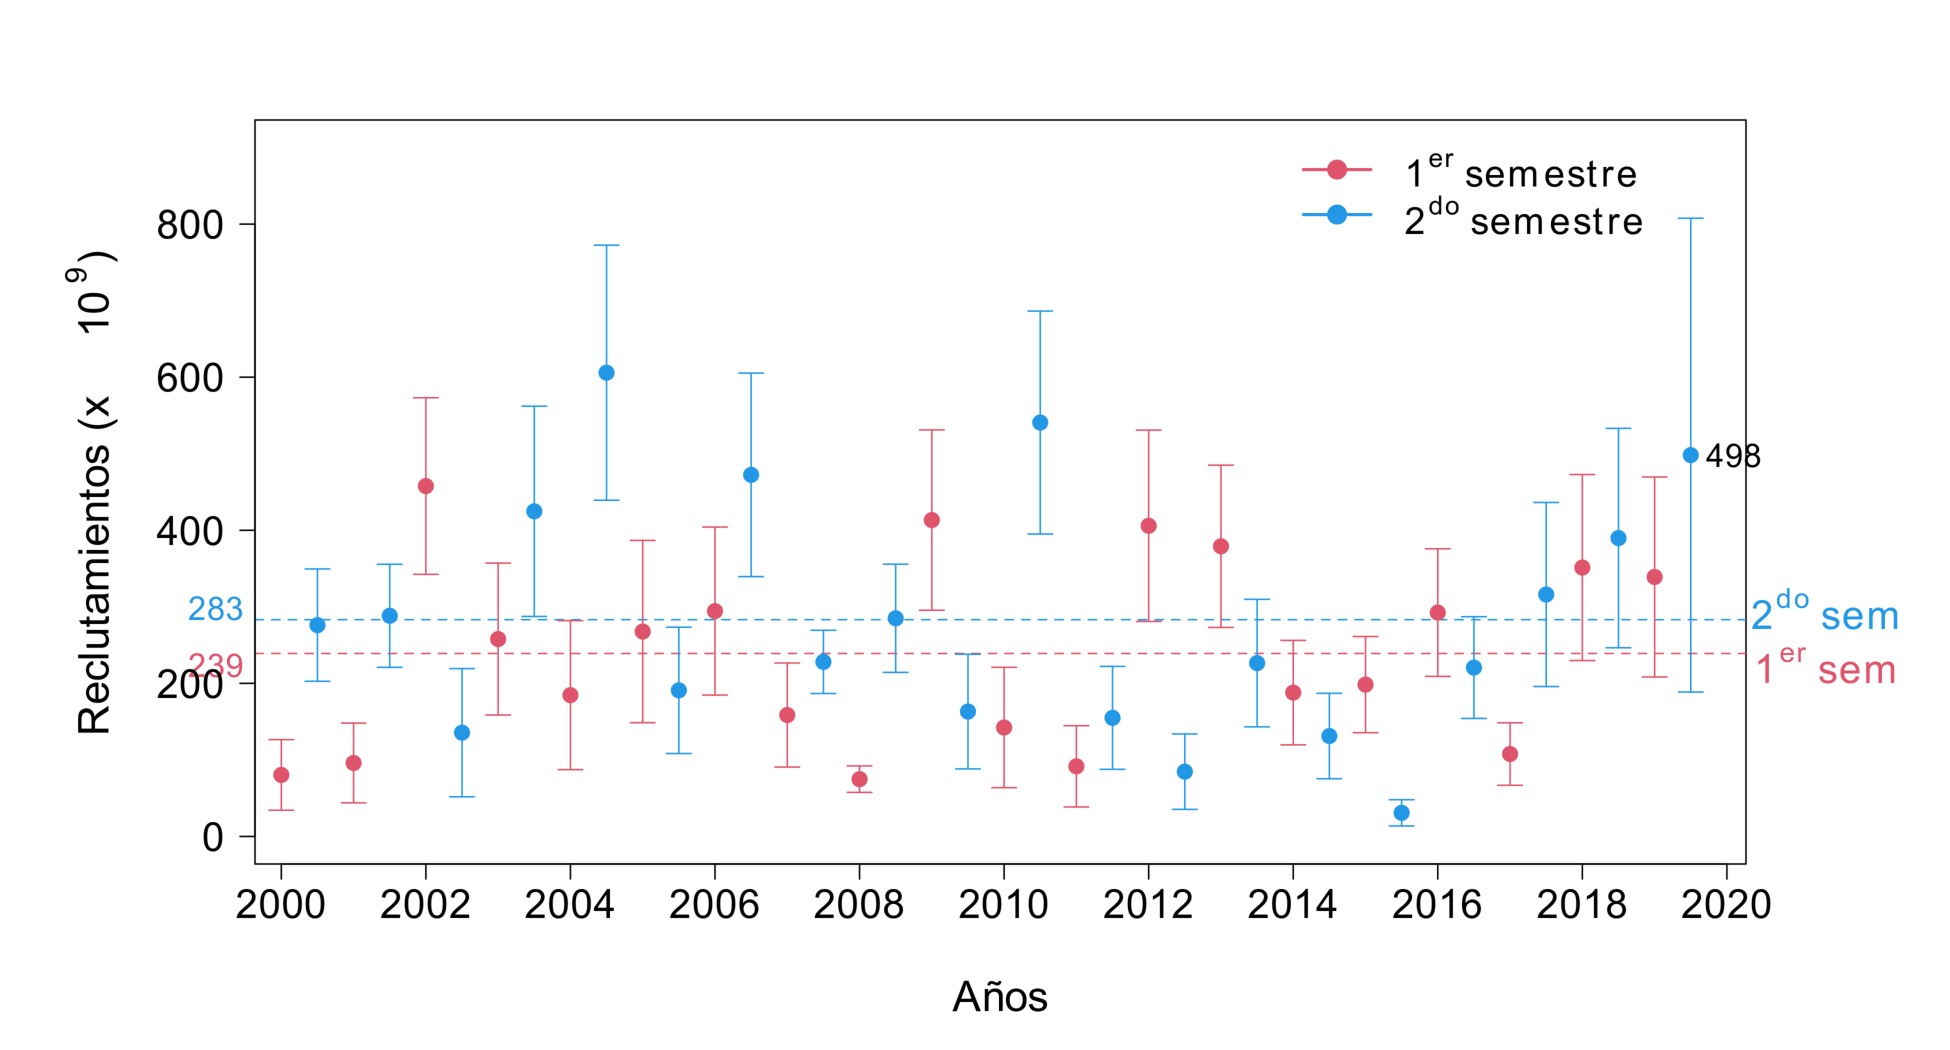
\includegraphics[width=15cm,height=8cm]{fig/figura10.pdf}
 \caption{Escenario de reclutamientos promedios diferenciado para el primer y segundo semestre empleados para proyectar el stock de anchoveta del sur de Per\'u y norte de Chile. Las l\'ineas punteadas indican los promedios para cada semestre.}
 \label{Fig10}
\end{figure}
\vspace{0.5cm}


Para proyectar el stock de anchoveta del sur de Per\'u y norte de Chile es
necesario incorporar los nuevos reclutas para cada semestre proyectado,
primer y segundo semestre del 2020 y 2021. La elecci\'on de los niveles de
reclutamientos que entran en cada semestre tiene fuertes implicancias en
los niveles poblacionales que se estimen en el futuro y en los niveles
de captura biol\'ogicamente aceptable debido principalmente al r\'apido
crecimiento (\textbf{Figura \ref{Fig04}}) y a una alta mortalidad natural
m\'as la mortalidad por pesca que genera el F$_{RMS}$. Dado que el
\'ultimo reclutamiento estimado por el modelo de evaluaci\'on tiene una alta
incertidumbre y m\'as el patr\'on retrospectivo en los reclutamientos, es
necesario aplicar el enfoque precautorio en la toma de decisi\'on inicial
(primer hito) y en su actualizaci\'on (segundo hito) sobre los niveles de
captura biol\'ogicamente aceptable, es decir, se podr\'ia considerar reducir
la longitud de la serie para el c\'alculo de los reclutamientos promedios
(elimando el \'ultimo año con alta incertidumbre) o penalizar el \'ultimo
reclutamiento estimado por el modelo de evaluaci\'on antes que se
proyecte la poblaci\'on del stock de anchoveta.\\


En la actualidad, la CBA considera un rango de valores (de 10 a 50\%)
basado en el riesgo de no alcanzar el objetivo de conservaci\'on. El
riesgo corresponde a una distribuci\'on de probabilidad acumulada y
representa la expectativa de sobrepasar la mortalidad por pesca que
conduce al objetivo de manejo, que es equivalente a mantener el stock
robusto. Dada la alta incertidumbre existente en el establecimiento de
la CBA en el proceso de asesor\'ia inicial, se recomienda utilizar un
nivel de riesgo muy inferior al 50\%.\\



\subsection{Penalizaci\'on del \'ultimo reclutamiento}


Dada la alta incertidumbre que se genera en el \'ultimo reclutamiento
estimado por el modelo de evaluaci\'on (\textbf{Figura \ref{Fig10}}) y
el fuerte patr\'on retrospectivo en los reclutamientos (\textbf{Figura 
\ref{Fig08}}), existe una alta probabilidad que al
incorporar nueva informaci\'on al modelo ($t+1$) el valor estimado para el 
reclutamiento ($t$) disminuya. Dada esta alta incertidumbre que se genera 
en el \'ultimo reclutamiento estimado por el modelo del evaluaci\'on y 
por el patr\'on retrospectivo en los reclutamientos, se proponen tres m\'etodos
para penalizar el \'ultimo reclutamiento estimado por el modelo:



\paragraph{a) l\'imite inferior del \'ultimo reclutamiento estimado}

\quad

En la \textbf{Figura \ref{Fig11}} se muestra el l\'imite inferior de la 
\'ultima estimaci\'on del reclutamiento hecha por el modelo, la que 
corresponde a 1.96 veces por la desviaci\'on est\'andar.


\paragraph{b) relaci\'on entre el reclutamiento y el desembarque}

\quad

Ocupando los datos de reclutamientos semestrales ($t$) estimados por el 
modelo de evaluaci\'on y los desembarques semestrales observados ($t+1$) en
la pesquer\'ia, se ajusta un modelo no-lineal para describir la relaci\'on
entre estas variables (\textbf{Figura \ref{Fig12}}). Los resultados del
modelo no-lineal son mostrado en la \textbf{Tabla \ref{Tab5}}.


\paragraph{c) l\'imite inferior de la \'ultima desviaci\'on de $R_{0}$}

\quad

Otra forma de penalizar el \'ultimo reclutamiento cuando se tiene por certeza
de su estimaci\'on es penalizar el \'ultimo desvi\'o de $R_{0}$. Este m\'etodo
es usado en la Organizaci\'on Regional de Pesca del Pac\'ifico Sur (SPRFMO) para
la evaluaci\'on de stock del jurel y consiste en usar el l\'imite inferior de la
\'ultima estimaci\'on de la desviaci\'on de $R_{0}$ desde el archivo .pin, y correr
el modelo de evaluaci\'on desde la \'ultima fase de estimaci\'on. En la
\textbf{Figura \ref{Fig13}} se muestra el esquema de estimaci\'on para este m\'etodo.  


\vspace{0.5cm}
\begin{figure}[htb!]
 \centering
 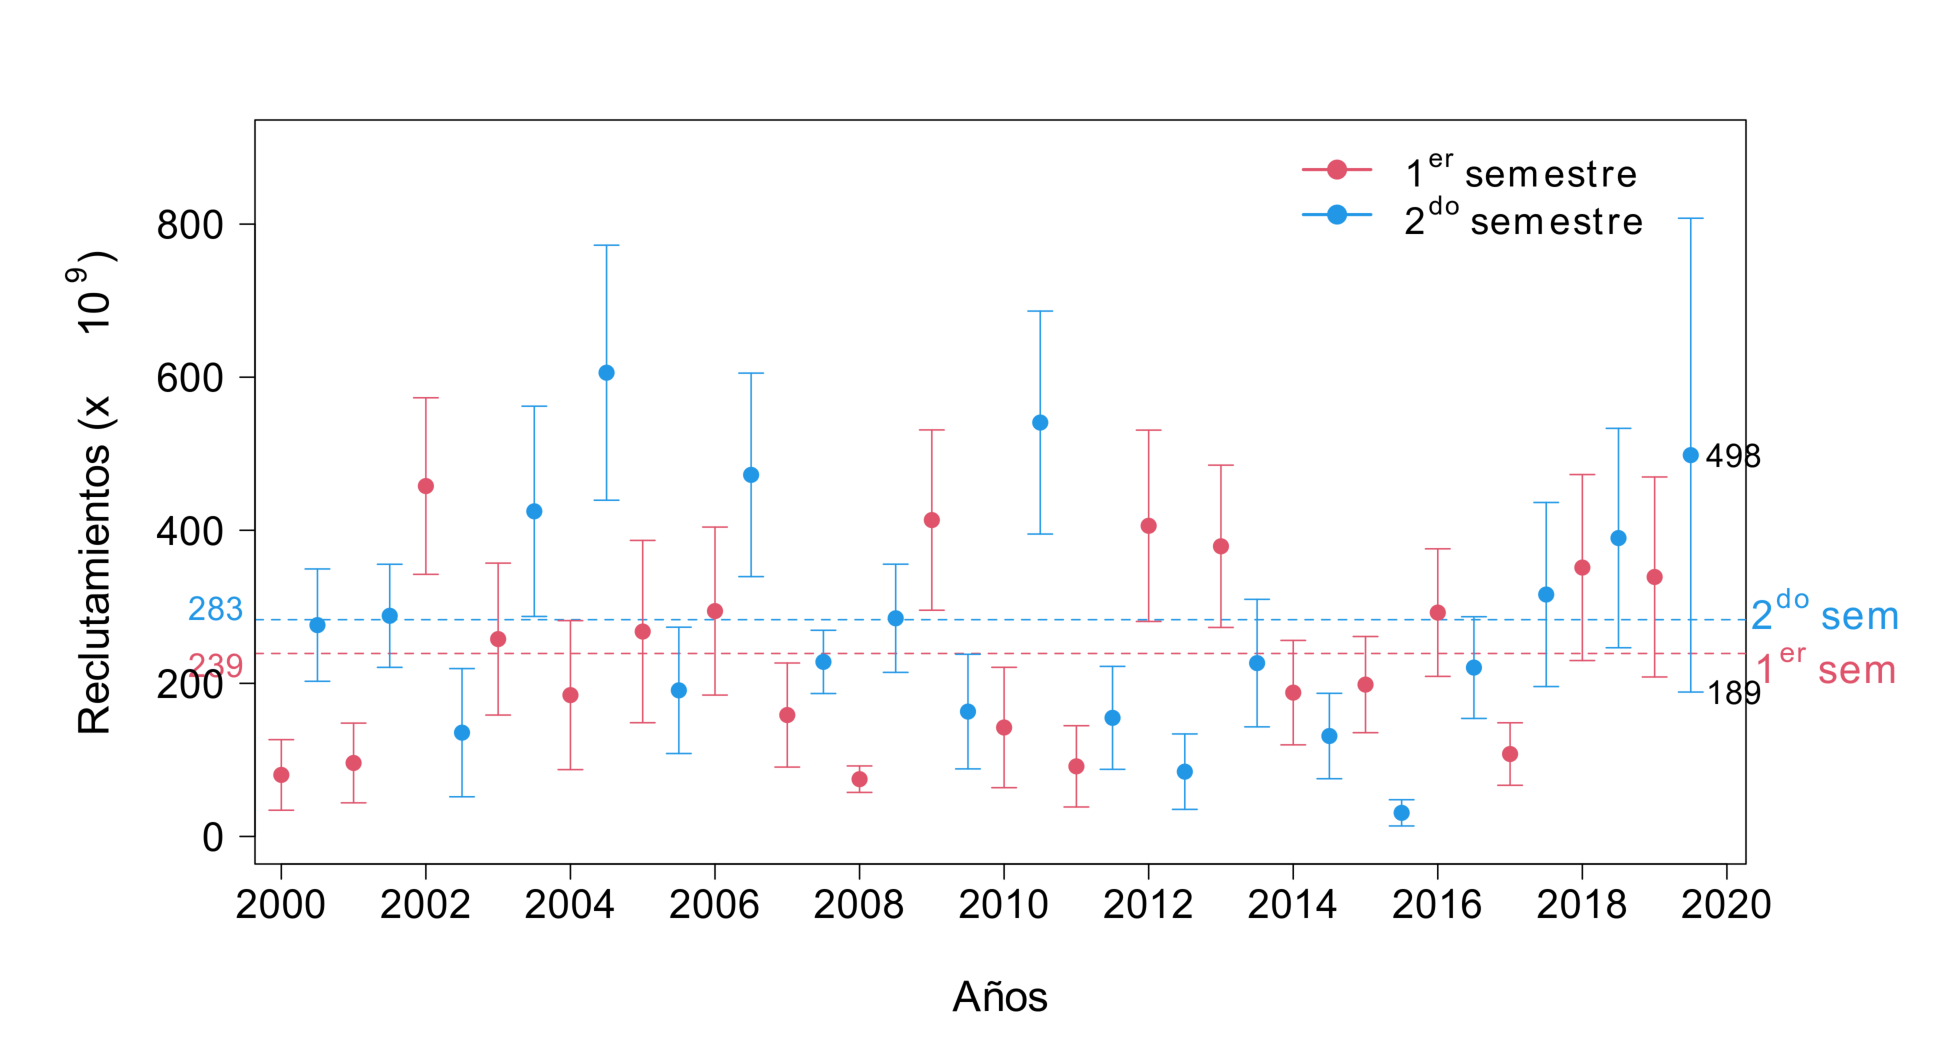
\includegraphics[width=14cm,height=7cm]{fig/figura11.pdf}
 \caption{Reclutamientos promedios diferenciado para el primer y segundo semestre empleados para proyectar el stock de anchoveta del sur de Per\'u y norte de Chile. Las l\'ineas punteadas indican los promedios para cada semestre.}
 \label{Fig11}
\end{figure}
\vspace{0.5cm}



\vspace{0.5cm}
\begin{figure}[htb!]
 \centering
 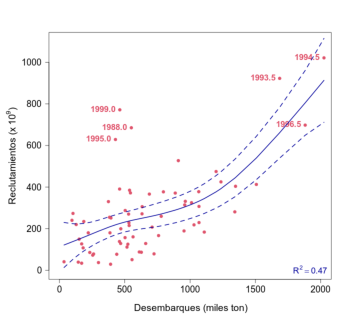
\includegraphics[width=12cm,height=8cm]{fig/figura12.pdf}
 \caption{Relaci\'on no-lineal entre los reclutamientos (t) y los desembarques totales (t+1) en escala semestral para el stock de anchoveta del sur de Per\'u y norte de Chile.}
 \label{Fig12}
\end{figure}
\vspace{0.5cm}



\vspace{0.5cm}
\begin{table}[!htbp] \centering 
\caption{Resultados del modelo no-lineal entre los reclutamientos ($t$) y los desembarques ($t+1$) en
escala semestral para el stock de anchoveta del sur de Per\'u y norte de Chile.}
\label{Tab5} 
\begin{tabular}{@{\extracolsep{1pt}}lrr} 
\\[-1.8ex]\hline 
\hline \\[-1.8ex] 
& \multicolumn{1}{r}{Param\'etrica} & \multicolumn{1}{r}{No param\'etrica} \\
\hline \\[-1.8ex] 
Intercepto & 270.821$^{***}$ \\ 
& (17.926) \\
s(desem) & & 2.845$^{***}$ \\
& & (3.528) \\ 
\hline \\[-1.8ex] 
Observaciones & & 69 \\ 
R$^{2}$ ajustado & & 0.465 \\ 
Log Likelihood & & $-$446.003 \\ 
UBRE & & 23,482.240 \\ 
\hline 
\hline \\[-1.8ex] 
\textit{Nota:} & & \multicolumn{1}{r}{$^{*}$p$<$0.1; $^{**}$p$<$0.05; $^{***}$p$<$0.01} \\ 
\end{tabular} 
\end{table}



\vspace{0.5cm}
\begin{figure}[htb!]
 \centering
 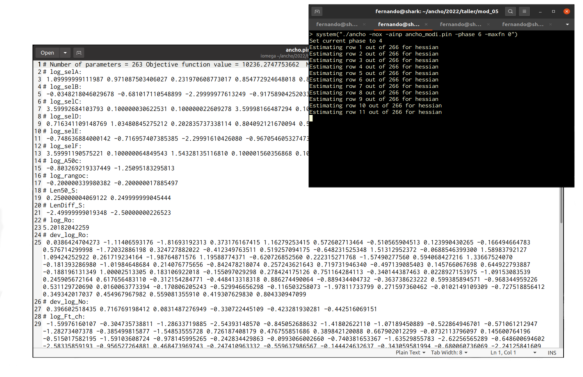
\includegraphics[width=14.5cm,height=10.5cm]{fig/figura13.pdf}
 \caption{Esquema que ilustra el archivo .pin y la modificiaci\'on del \'ultima estimaci\'on de la
 desviaci\'on de $R_{0}$, y la consola de comando donde se ejecuta esa instrucci\'on.}
 \label{Fig13}
\end{figure}
\vspace{0.5cm}



\clearpage
\newpage
%\pagebreak

\section{RESULTADOS}


\subsection{Efecto en la incorporaci\'on de nuevos datos}


El gran desaf\'io que presentan los peque\~{n}os peces pel\'agicos a nivel
mundial, y m\'as a\'un para la anchoveta del norte de Chile que presenta una
r\'apida tasa de crecimiento con una alta mortalidad natural, es intentar predecir los
reclutamientos futuros durante la proyecci\'on del stock. Esto se complica a\'un m\'as,
ya que el modelo de evaluaci\'on de stock presenta una tendencia a sobre-estimar
los reclutamientos del primer hito de asesor\'ia cuando se incorporan nuevos datos
en el segundo hito de asesor\'ia (panel intermedio, \textbf{Figura \ref{Fig14}}). Este patr\'on
retrospectivo en los reclutamientos (\textbf{Figura \ref{Fig07} y \ref{Fig08}}) hace
necesario plantearse algunos escenarios sobre los supuestos en los reclutamientos
que ser\'an ingresados durante la proyecci\'on del stock de anchoveta, tanto para el
primer hito de asesor\'ia (septiembre), como en el segundo hito (marzo) de
asesora\'ia.


\vspace{0.5cm}
\begin{figure}[htb!]
 \centering
 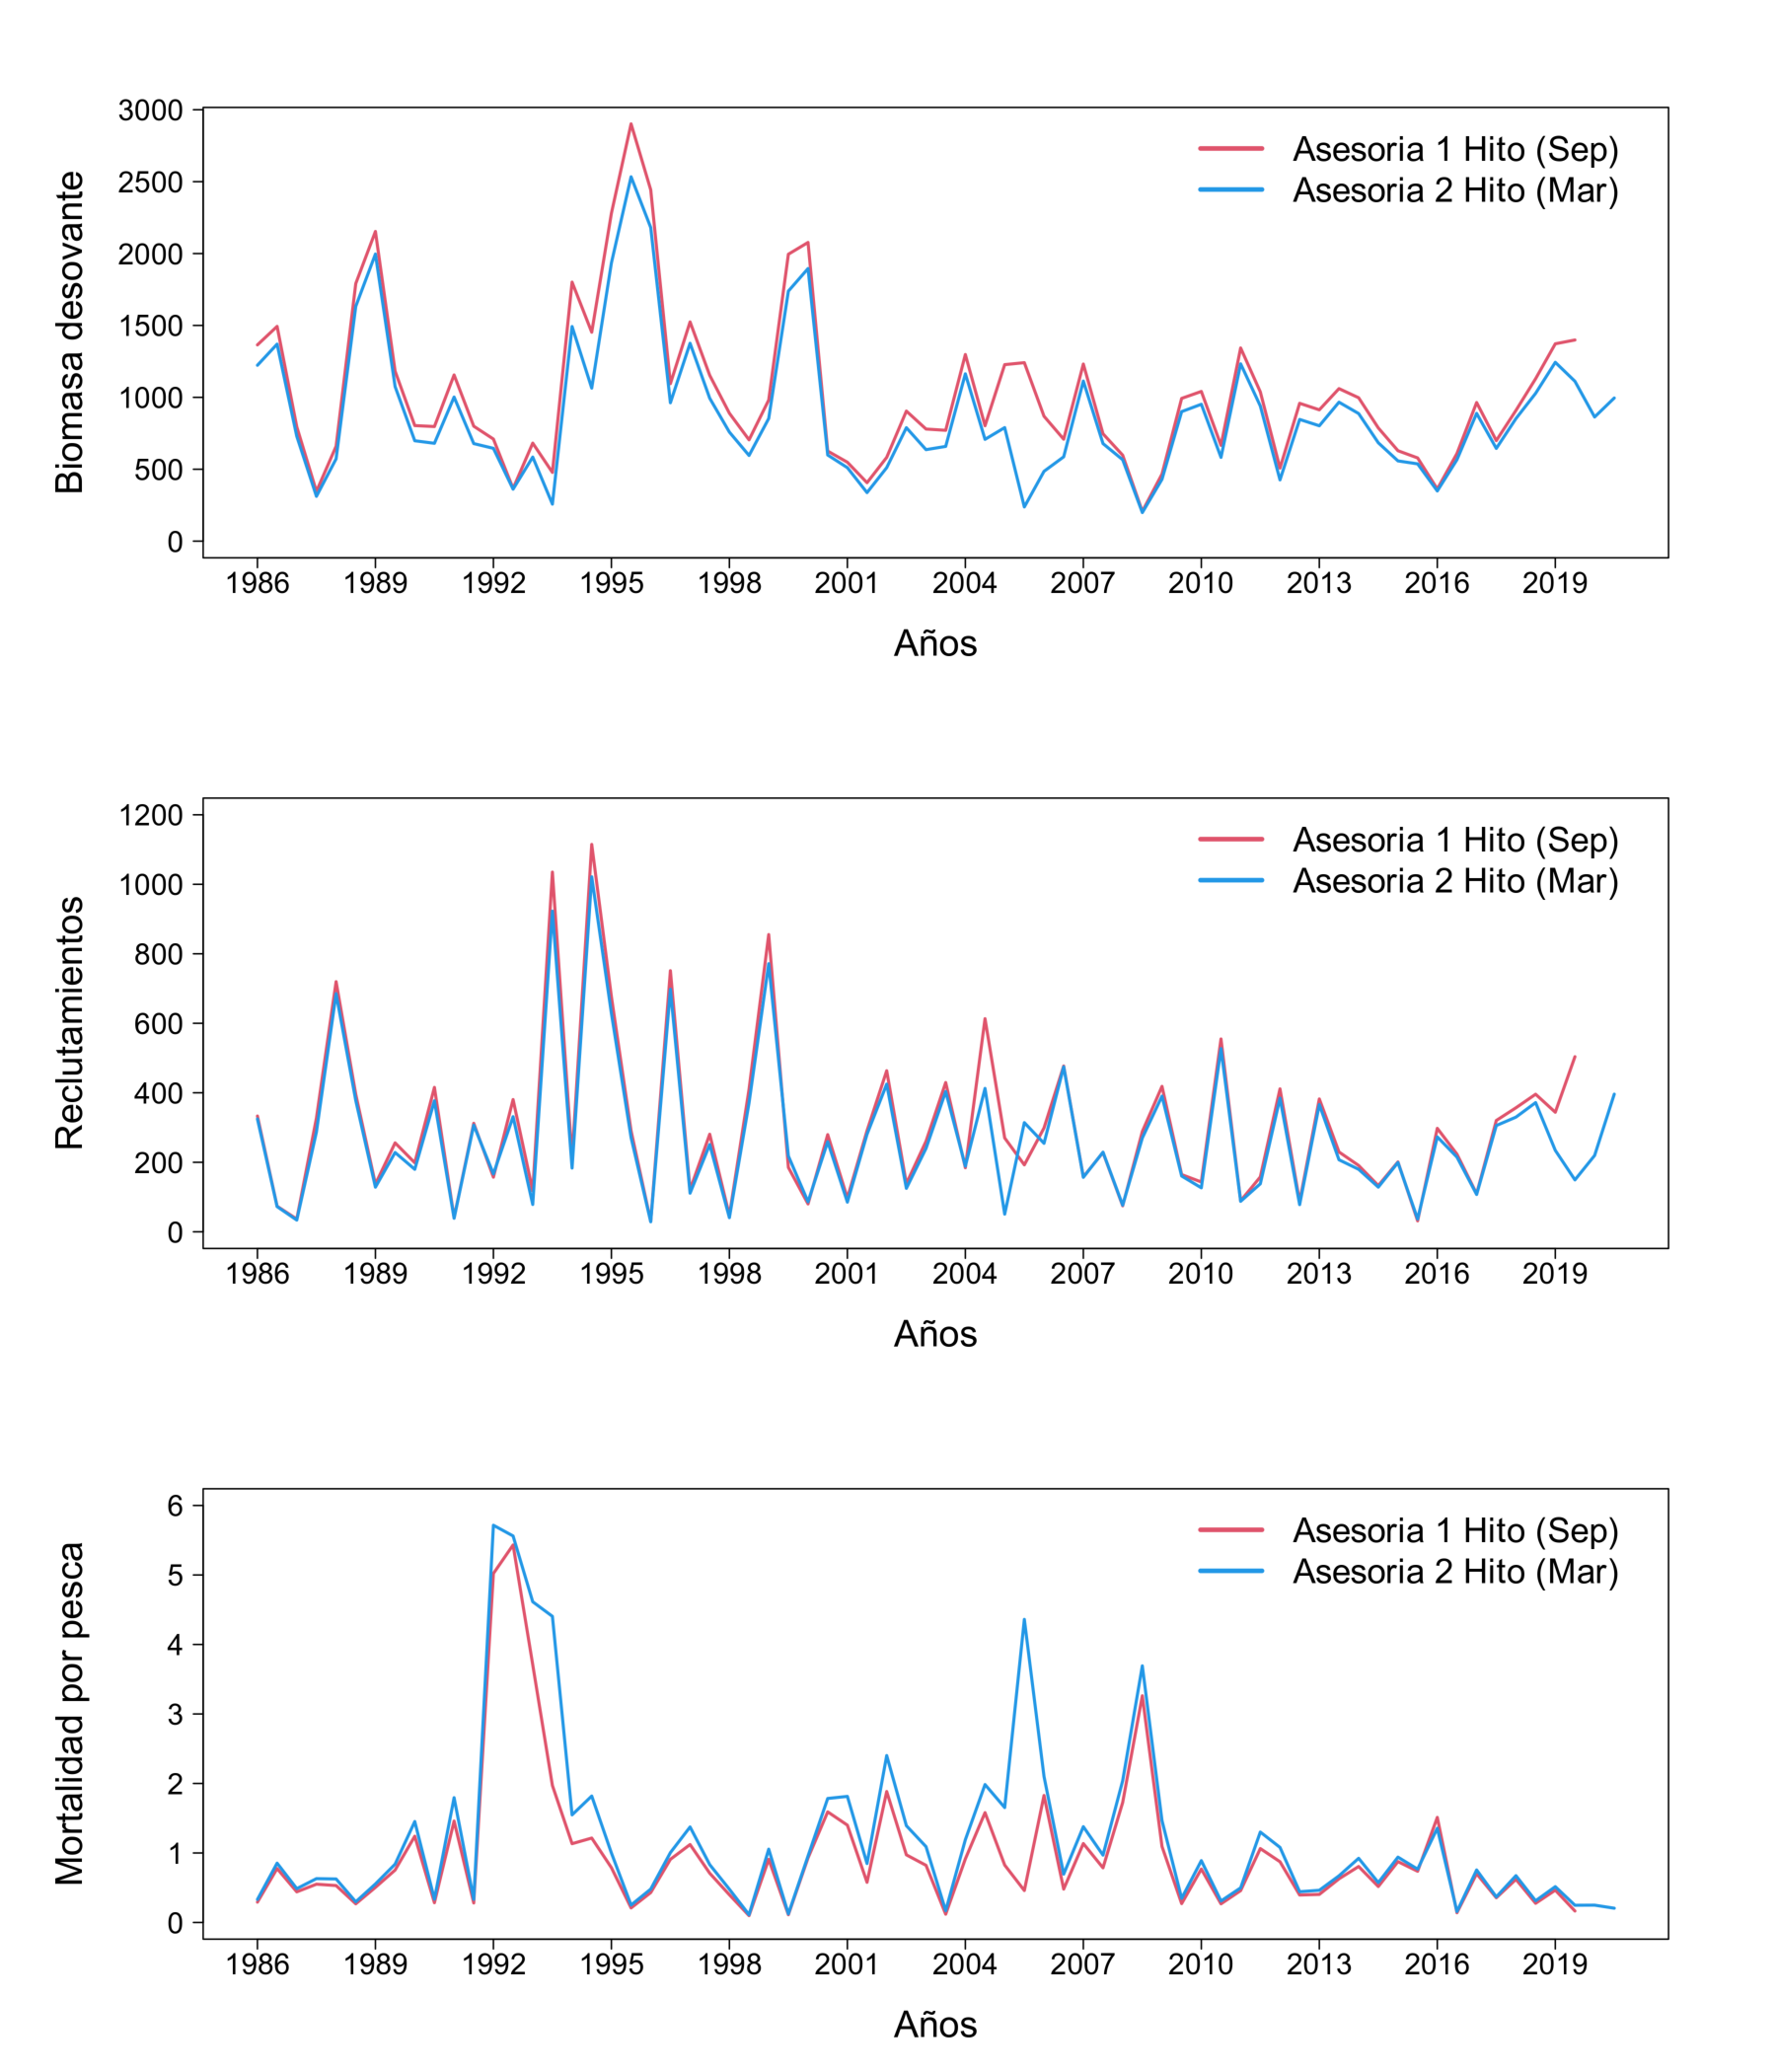
\includegraphics[width=16cm,height=13cm]{fig/figura14.pdf}
 \caption{Estimaciones de las principales variables de estado durante el ciclo de asesor\'ia anual. El Hito 1 corresponde a la asesor\'ia de septiembre 2020 y el Hito 2 a la asesor\'ia del marzo del 2021.}
 \label{Fig14}
\end{figure}


\subsection{Revisi\'on del proceso de estimaci\'on de CBA de anchoveta norte}

\quad

El establecimiento de la CBA anual para el stock de la anchoveta
del sur de Per\'u y norte de Chile tiene dos hitos: i) el primer hito de
asesor\'ia que ocurre en octubre de cada a\~{n}o, donde es necesario proyectar el
stock de anchoveta cuatro semestres para estimar la CBA anual, y adem\'as durante el
primer y segundo semestre proyectado la mortalidad por pesca conocida. 
Y ii) el segundo hito de asesor\'ia que ocurre en marzo-abril de cada
a\~{n}o, y es necesario proyectar el stock de anchoveta dos semestres para
estimar la CBA anual. En cada uno de estos hitos es
necesario hacer supuestos sobre los niveles de reclutamientos (n\'umero de
individuos) que ser\'an ingresados en cada uno de los semestres
proyectados. Estos niveles de reclutamientos podri\'an
corresponder a un promedio de ciertos reclutamientos que ocurrieron en
un periodo determinado (longitud de la serie) de tiempo, diferenciado por
semestres o un patr\'on inherente que ocurre dentro del a\~{n}o (sem1 $>$
sem2 o sem1 $<$ sem2). O podr\'iamos hacer alg\'un tipo de penalizaci\'on
del \'ultimo reclutamiento estimado por el modelo dado el patr\'on retrospectivo
que se observa en los reclutamientos (\textbf{Figura \ref{Fig08}}).
Para el caso de penalizar el reclutamiento, se consideran tres m\'etodos: i) el l\'imite inferior
del intervalo de confianza estimado por el modelo para el \'ultimo reclutamiento,
ii) predicr el reclutamiento desde una relaci\'on no-lineal entre el reclutamiento
($t$) y el desembarque ($t+1$), y iii) el l\'imite inferior del intervalo de confianza
estimado por el modelo para la \'ultima desviaci\'on de $R_{0}$. Para cada uno de los
hitos de asesor\'ia, se asumen que los reclutamientos ingresados en cada uno de los semestres
proyectados es considerado como un evento independiente de un semestre a otro.

Los resultados mostrados a continuaci\'on corresponde a modo de ejemplo,
donde el modelo de evaluaci\'on entrega estimaciones de todos los grupos
etarios hasta el 2019.5, se considera la mortalidad por pesca total
(flota chilena + flota peruana) y los pesos medios del \'ultimo semestre.
La mortalidad por pesca total es ponderada por la mortalidad por pesca
que produce el RMS, equivalente al 55\%BDPR.


\subsubsection{Primer hito}

\paragraph{a) 4 semestres proyectados}

\quad

Para el primer hito de asesor\'ia se evaluaron los siguientes escenarios
\textbf{Tabla \ref{Tab6}} para 4 semestres proyectados. Los resultados de
las proyecciones muestran que la biomasa desovante deber\'ia fluctuar entre
un mill\'on 776 mil toneladas y 927 mil toneladas para el escenario E1, y
valores un poco menores para el escenario E2. Para el escenario E3, la biomasa
desovante deber\'ia fluctuar entre un mill\'on 225 mil toneladas y 813 mil
toneladas, y valores un poco menores para el escenario E4. Para el 
escenario E5, la biomasa desovante deber\'ia fluctuar entre un mill\'on
158 mil toneladas y 799 mil toneladas, y valores un poco menores para el
escenario E6, el cu\'al registro los menores valores para todos los
escenarios evaluados. Finalmente, para el escenario E7, la biomasa
desovante deber\'ia fluctuar entre un mill\'on 388 mil toneladas y 852
mil toneladas, y valores un poco menores para el escenario E8 (\textbf{Figura \ref{Fig15}}).\\

Para todos los escenarios evaluados durante el primer y segundo semestre proyectado,
la captura tienen valores muy similares, debido a que esta es conocida
(\textbf{Figura \ref{Fig15}} y \textbf{Tabla \ref{Tab7}}). Para el
tercer semestre proyectado la captura registra un valor m\'aximo de 432
mil toneladas para el escenario E1 y un valor m\'inimo de 398 mil
toneladas para el escenario E6. Y para el cuatro semestre proyectado la
captura registra un valor m\'aximo de 343 mil toneladas para el escenario
E1 y un valor m\'inimo de 326 mil toneladas para el escenario E2, E4 y E6. En
t\'erminos de la reducci\'on de la biomasa desovante de largo plazo del
stock de anchoveta, todos los escenarios evaluados convergen al final de
la proyecci\'on a un valor por sobre el objetivo de manejo pesquero,
indicando que el stock de anchoveta es altamente productivo dado los
niveles de reclutamientos ingresados durante la proyecci\'on
(\textbf{Figura \ref{Fig15}}).\\



\vspace{0.5cm}
\begin{table}[htb!]
 \caption{Escenarios de proyecci\'on (4 semestres) usados en el primer hito de asesor\'ia.}
 \label{Tab6}
 \centering
 \small
 \begin{tabular}{ll}
 \hline\noalign{\vskip 0.1cm}
 Escenario & Descripci\'on \\
 \hline\noalign{\vskip 0.1cm}
 E1  &  Reclutamientos promedios desde el 2000 hasta el 2019.5  \\
 E2  &  Reclutamientos promedios desde el 2000 hasta el 2018.5  \\
 E3  &  E1 + penalizaci\'on \'ultimo reclutamiento (2019.5) Np(1)=188.6  \\
 E4  &  E2 + penalizaci\'on \'ultimo reclutamiento (2019.5) Np(1)=188.6 \\
 E5  &  E1 + penalizaci\'on \'ultimo reclutamiento (relaci\'on) Np(1)=149.5 \\
 E6  &  E2 + penalizaci\'on \'ultimo reclutamiento (relaci\'on) Np(1)=149.5 \\
 E7  &  E1 + penalizaci\'on \'ultimo desviaciones de $R_{0}$=0.8-1.96*0.3 \\
 E8  &  E2 + penalizaci\'on \'ultimo desviaciones de $R_{0}$=0.8-1.96*0.3 \\
 \hline
 \end{tabular}
\end{table}
\vspace{0.5cm}


\vspace{0.5cm}
\begin{figure}[htb!]
 \centering
 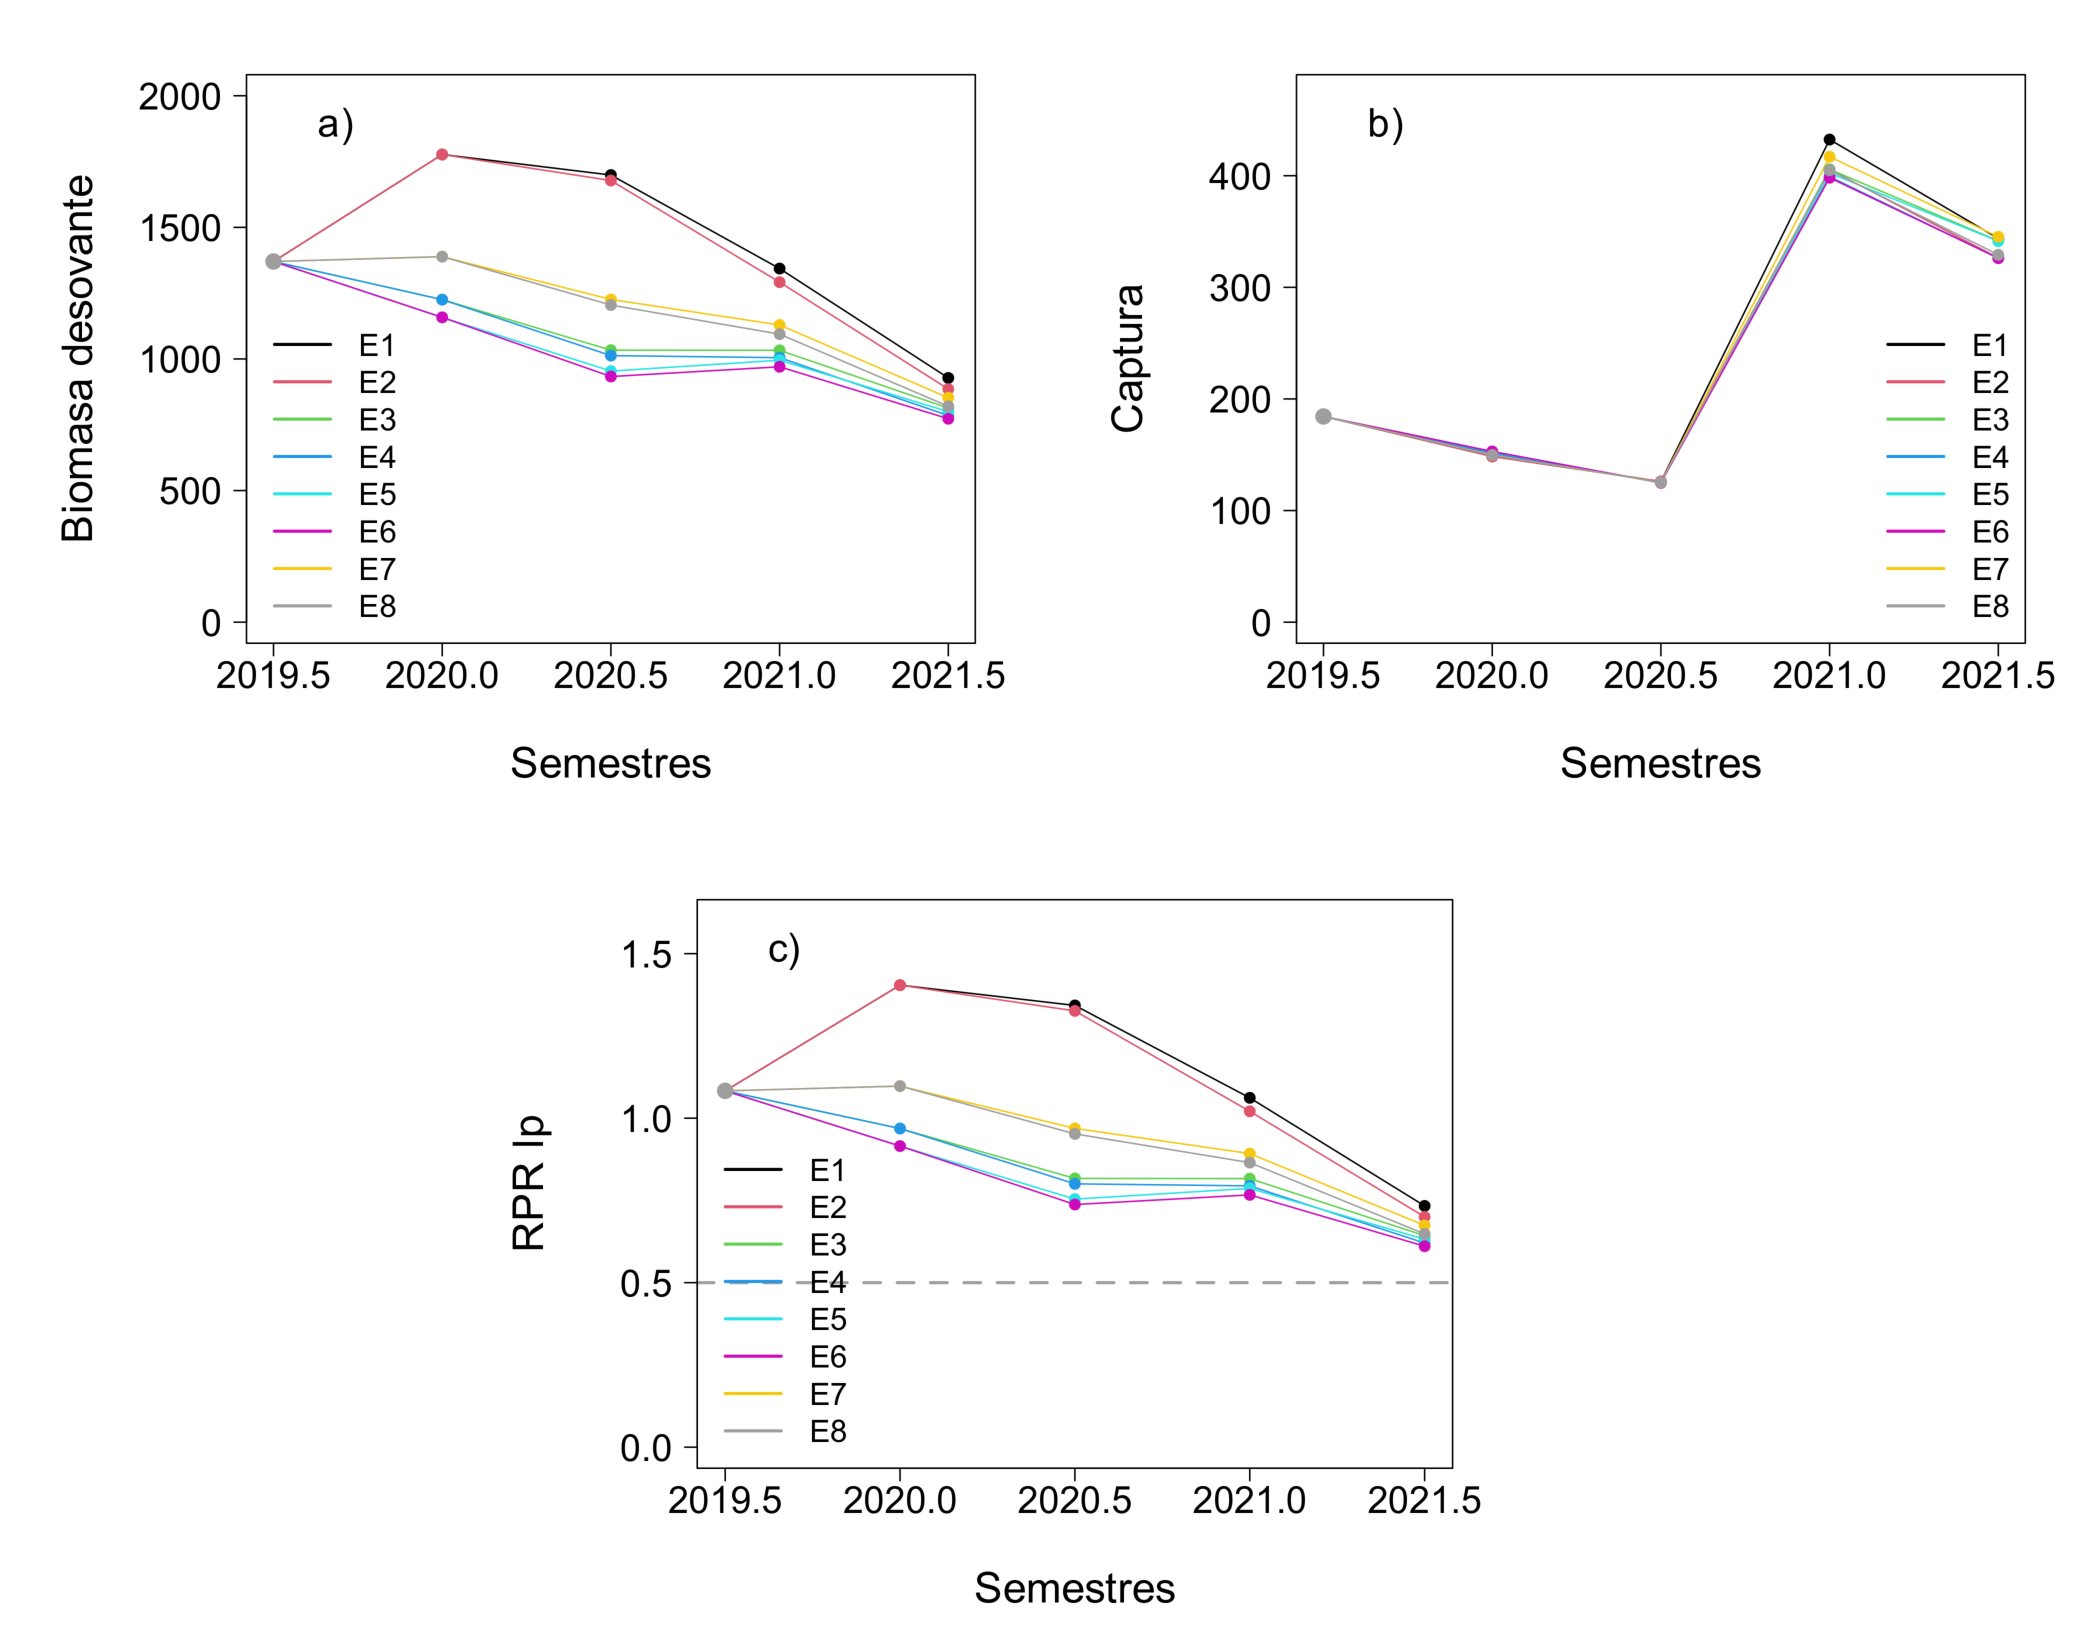
\includegraphics[width=14cm,height=12cm]{fig/figura15.pdf}
 \caption{Biomasa desovante (a), capturas (b) y RPR largo plazao (c) proyectado durante 4 semestres para el primer hito de asesor\'ia.}
 \label{Fig15}
\end{figure}
\vspace{0.5cm}



\vspace{0.5cm}
\begin{table}[htb!]
 \caption{CBA semestral proyectada (2020.0-2021.5) y anual para el 2021 para el stock de anchoveta dado el criterio del F=F$_{RMS}$ y los diferentes escenarios evaluados.}
 \label{Tab7}
 \centering
 \small
 \begin{tabular}{lccccc}
 \hline\noalign{\vskip 0.1cm}
 Escenario & 2020.0 & 2020.5 & 2021.0 & 2021.5 & 2021$_{TOT}$ \\
 \hline\noalign{\vskip 0.1cm}
 E1  & 148.5 & 125.9 & 432.4 & 343.8 & 776.2  \\
 E2  & 148.5 & 126.1 & 405.6 & 326.3 & 731.9 \\
 E3  & 151.4 & 124.9 & 405.6 & 341.6 & 747.2 \\
 E4  & 151.4 & 125.0 & 399.1 & 326.1 & 725.2  \\
 E5  & 152.9 & 124.7 & 402.3 & 341.3 & 743.6  \\
 E6  & 152.9 & 124.8 & 398.2 & 326.1 & 724.3  \\
 E7  & 149.7 & 125.3 & 417.0 & 345.3 & 762.3  \\
 E8  & 149.7 & 125.4 & 404.8 & 329.1 & 733.9  \\
 \hline
 \end{tabular}
\end{table}
\vspace{0.5cm}

\pagebreak


\paragraph{b) 3 semestres proyectados}


\quad

Para proyectar el stock de anchoveta durante 3 semestres se evaluaron los siguientes
escenarios \textbf{Tabla \ref{Tab8}}. Los resultados de las proyecciones muestran
que la biomasa desovante deber\'ia flucturar entre tres millones 929 mil toneladas y
un mill\'on 981 mil toneladas para el escenario S1, y valores un poco menores para el
escenario S2. Para el escenario S3, la biomasa desovante deber\'ia fluctuar entre un
mill\'on 252 mil toneladas y 835 mil toneladas, y valores un poco menores para el
escenario S4. Para el  escenario S5, la biomasa desovante deber\'ia fluctuar entre un
mill\'on 85 mil toneladas y 764 mil toneladas, y valores un poco menores para el
escenario S6, el cu\'al registro los menores valores para todos los escenarios evaluados.
Finalmente, para el escenario S7, la biomasa desovante deber\'ia fluctuar entre dos millones
194 mil toneladas y un mill\'on 241 mil toneladas, y valores un poco menores para el 
escenario S8 (\textbf{Figura \ref{Fig16}}).\\


Para todos los escenarios evaluados durante el primer semestre proyectado,
la captura tienen valores muy similares, debido a que esta es conocida
(\textbf{Tabla \ref{Tab9}}). Para el
segundo semestre proyectado la captura registra un valor m\'aximo de 801
mil toneladas para el escenario S1 y un valor m\'inimo de 318 mil
toneladas para el escenario S5. Y para el tercer semestre proyectado la
captura registra un valor m\'aximo de 365 mil toneladas para el escenario
S1 y un valor m\'inimo de 342 mil toneladas para el escenario S4 y S6. En
t\'erminos de la reducci\'on de la biomasa desovante de largo plazo del
stock de anchoveta, todos los escenarios evaluados convergen al final de
la proyecci\'on a un valor por sobre el objetivo de manejo pesquero,
indicando que el stock de anchoveta es altamente productivo dado los
niveles de reclutamientos ingresados durante la proyecci\'on
(\textbf{Figura \ref{Fig16}}).\\



\vspace{0.5cm}
\begin{table}[htb!]
 \caption{Escenarios de proyecci\'on (3 semestres) usados en el primer hito de asesor\'ia.}
 \label{Tab8}
 \centering
 \small
 \begin{tabular}{ll}
 \hline\noalign{\vskip 0.1cm}
 Escenario & Descripci\'on \\
 \hline\noalign{\vskip 0.1cm}
 S1  &  Reclutamientos promedios desde el 2000 hasta el 2019.5  \\
 S2  &  Reclutamientos promedios desde el 2000 hasta el 2018.5  \\
 S3  &  S1 + penalizaci\'on \'ultimo reclutamiento (2019.5) Np(1)=250.2  \\
 S4  &  S2 + penalizaci\'on \'ultimo reclutamiento (2019.5) Np(1)=250.2 \\
 S5  &  S1 + penalizaci\'on \'ultimo reclutamiento (relaci\'on) Np(1)=149.5 \\
 S6  &  S2 + penalizaci\'on \'ultimo reclutamiento (relaci\'on) Np(1)=149.5 \\
 S7  &  S1 + penalizaci\'on \'ultimo desviaciones de $R_{0}$=2.1-1.96*0.4 \\
 S8  &  S2 + penalizaci\'on \'ultimo desviaciones de $R_{0}$=2.1-1.96*0.4 \\
 \hline
 \end{tabular}
\end{table}
\vspace{0.5cm}



\vspace{0.5cm}
\begin{figure}[htb!]
 \centering
 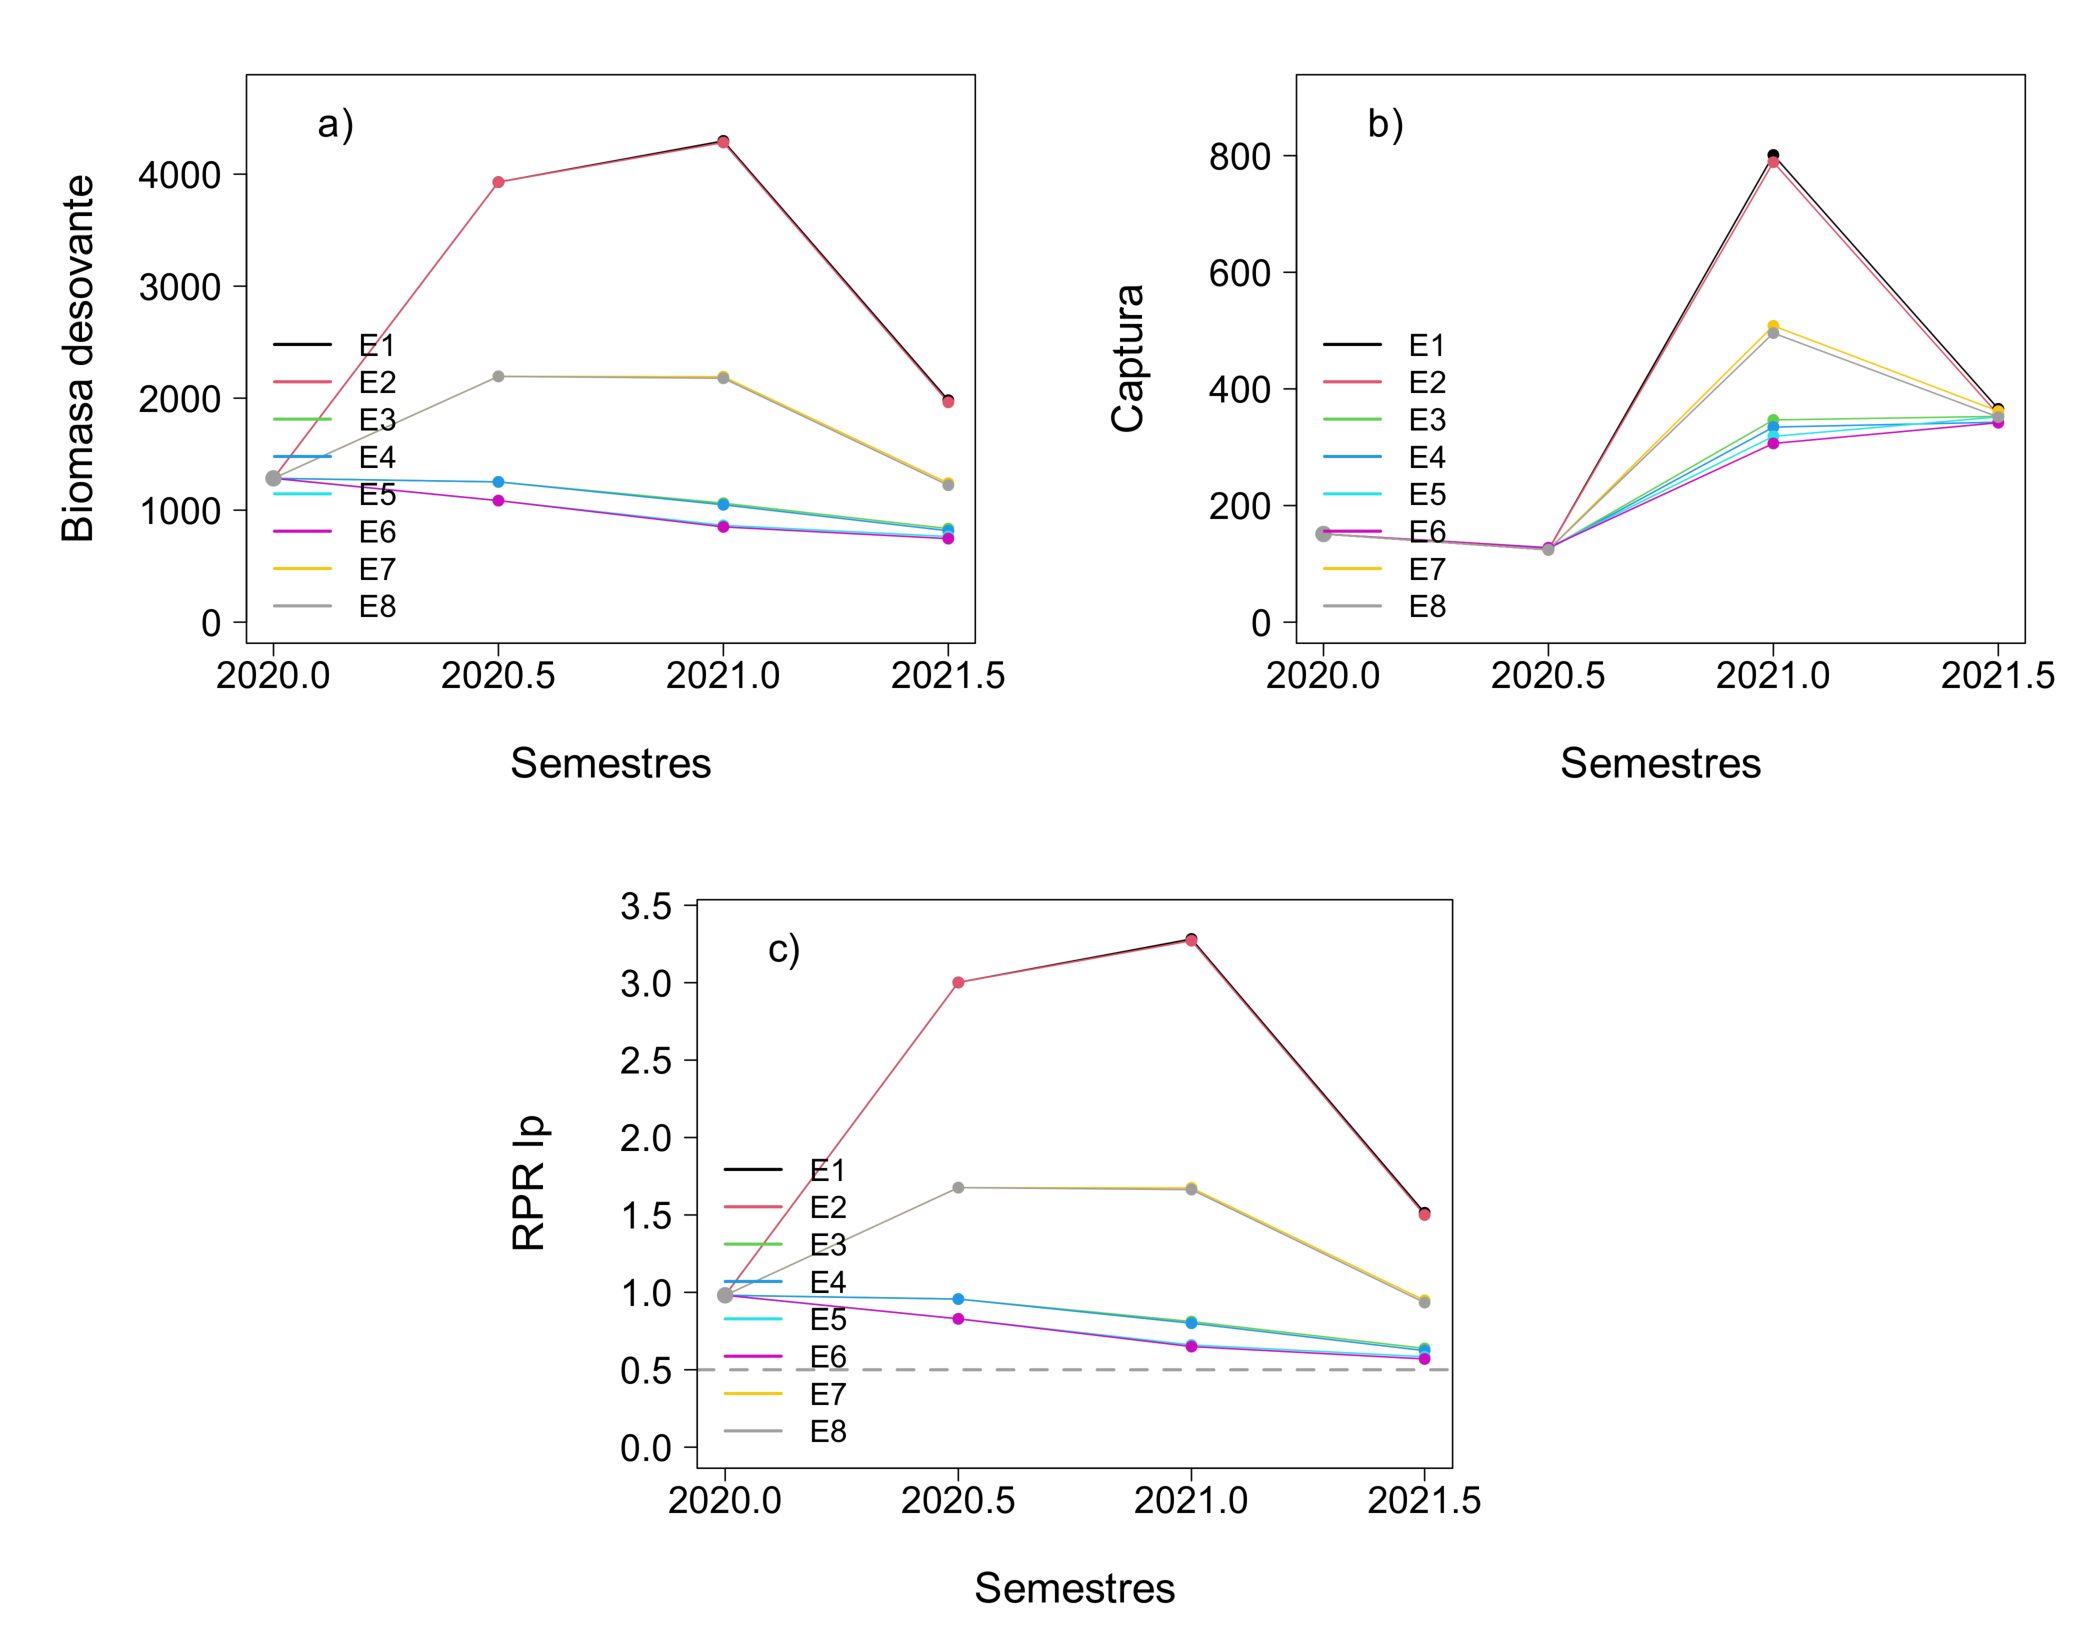
\includegraphics[width=14cm,height=12cm]{fig/figura16.pdf}
 \caption{Biomasa desovante (a), capturas (b) y RPR largo plazao (c) proyectado durante 3 semestres para el primer hito de asesor\'ia.}
 \label{Fig16}
\end{figure}
\vspace{0.5cm}



\vspace{0.5cm}
\begin{table}[htb!]
 \caption{CBA semestral proyectada (2020.5-2021.5) y anual para el 2021 para el stock de anchoveta dado el criterio del F=F$_{RMS}$ y los diferentes escenarios evaluados.}
 \label{Tab9}
 \centering
 \small
 \begin{tabular}{lcccc}
 \hline\noalign{\vskip 0.1cm}
 Escenario & 2020.5 & 2021.0 & 2021.5 & 2021$_{TOT}$ \\
 \hline\noalign{\vskip 0.1cm}
 S1  & 124.0 & 801.1 & 365.8 & 1166.9  \\
 S2  & 124.0 & 788.7 & 355.8 & 1144.5 \\
 S3  & 125.5 & 346.8 & 352.9 & 699.7 \\
 S4  & 125.5 & 334.5 & 342.9 & 677.4  \\
 S5  & 127.7 & 318.7 & 352.0 & 670.7  \\
 S6  & 127.7 & 306.5 & 342.0 & 648.5  \\
 S7  & 124.2 & 508.2 & 361.8 & 870.0  \\
 S8  & 124.2 & 495.7 & 351.6 & 847.3  \\
 \hline
 \end{tabular}
\end{table}
\vspace{0.5cm}



\subsubsection{Aporte de cada grupo de edad a la captura proyectada por semestre}

\paragraph{a) 4 semestres proyectados}

\quad

Durante la proyecci\'on del stock de anchoveta se estim\'o la captura en
n\'umero de individuos por grupo de edad (Baranov, 1918), y luego fue
dividida por la suma total de todos los grupos de edad. Este porcentaje
por grupo de edad en la captura es presentado en las
\textbf{Tabla \ref{Tab10}}, \textbf{Tabla \ref{Tab11}},
\textbf{Tabla \ref{Tab12}}, \textbf{Tabla \ref{Tab13}},\textbf{Tabla \ref{Tab14}},
\textbf{Tabla \ref{Tab15}},\textbf{Tabla \ref{Tab16}} y \textbf{Tabla \ref{Tab17}}
para el escenario E1, E2, E3, E4, E5, E6, E7 y E8 respectivamente. Independiente del
escenario evaluado, el grupo de edad 1 (6 meses) es el que mayor porcentaje aporta a
la captura semestral. Para el escenario E1 y E2 este valor var\'ia entre
un 78\% y un 91\%, para el escenario E3 y E4 este valor varia entre un
78\% y un 83\%, para el escenario E5 y E6 este valor varia entre un 74\% y 87\% y
para el escenario E7 y E8 este valor varia entre un 84\% y 85\%. En general, los
grupos de edades 0 (reclutas), 1 (6 meses) y 2 (1 a\~{n}o) aportan el 100\% de la
captural semestral para todos los escenarios evaluados durante la proyecci\'on del
stock de anchoveta.\\

\vspace{0.5cm}
\begin{table}[htb!]
 \caption{Porcentaje por grupo de edad en la captura proyectada (2020.0-2021.5) para el escenario E1.}
 \label{Tab10}
 \centering
 \small
 \begin{tabular}{lcccc}
 \hline\noalign{\vskip 0.1cm}
 Edad & 2020.0 & 2020.5 & 2021.0 & 2021.5 \\
 \hline\noalign{\vskip 0.1cm}
 0 & 0.041 & 0.090 & 0.088 & 0.123  \\
 \rowcolor{Gray}
 1 & 0.914 & 0.787 & 0.848 & 0.831 \\
 2 & 0.043 & 0.120 & 0.059 & 0.042 \\
 3 & 0.001 & 0.002 & 0.003 & 0.001  \\
 \hline
 \rowcolor{Gray}
 Suma(0:2) & 0.999 & 0.998 & 0.996 & 0.998 \\
 \hline
 \end{tabular}
\end{table}
\vspace{0.5cm}


\vspace{0.5cm}
\begin{table}[htb!]
 \caption{Porcentaje por grupo de edad en la captura proyectada (2020.0-2021.5) para el escenario E2.}
 \label{Tab11}
 \centering
 \small
 \begin{tabular}{lcccc}
 \hline\noalign{\vskip 0.1cm}
 Edad & 2020.0 & 2020.5 & 2021.0 & 2021.5 \\
 \hline\noalign{\vskip 0.1cm}
 0 & 0.039 & 0.088 & 0.089 & 0.122  \\
 \rowcolor{Gray}
 1 & 0.916 & 0.783 & 0.846 & 0.833 \\
 2 & 0.043 & 0.126 & 0.060 & 0.042 \\
 3 & 0.001 & 0.002 & 0.003 & 0.001  \\
 \hline
 \rowcolor{Gray}
 Suma(0:2) & 0.999 & 0.997 & 0.996 & 0.998 \\
 \hline
 \end{tabular}
\end{table}
\vspace{0.5cm}



\vspace{0.5cm}
\begin{table}[htb!]
 \caption{Porcentaje por grupo de edad en la captura proyectada (2020.0-2021.5) para el escenario E3.}
 \label{Tab12}
 \centering
 \small
 \begin{tabular}{lcccc}
 \hline\noalign{\vskip 0.1cm}
 Edad & 2020.0 & 2020.5 & 2021.0 & 2021.5 \\
 \hline\noalign{\vskip 0.1cm}
 0 & 0.103 & 0.095 & 0.093 & 0.118  \\
 \rowcolor{Gray}
 1 & 0.788 & 0.861 & 0.845 & 0.839 \\
 2 & 0.105 & 0.041 & 0.059 & 0.040 \\
 3 & 0.002 & 0.002 & 0.001 & 0.001  \\
 \hline
 \rowcolor{Gray}
 Suma(0:2) & 0.997 & 0.997 & 0.998 & 0.998 \\
 \hline
 \end{tabular}
\end{table}
\vspace{0.5cm}



\vspace{0.5cm}
\begin{table}[htb!]
 \caption{Porcentaje por grupo de edad en la captura proyectada (2020.0-2021.5) para el escenario E4.}
 \label{Tab13}
 \centering
 \small
 \begin{tabular}{lcccc}
 \hline\noalign{\vskip 0.1cm}
 Edad & 2020.0 & 2020.5 & 2021.0 & 2021.5 \\
 \hline\noalign{\vskip 0.1cm}
 0 & 0.099 & 0.099 & 0.090 & 0.122  \\
 \rowcolor{Gray}
 1 & 0.792 & 0.855 & 0.851 & 0.833 \\
 2 & 0.106 & 0.043 & 0.056 & 0.042 \\
 3 & 0.002 & 0.002 & 0.001 & 0.001  \\
 \hline
 \rowcolor{Gray}
 Suma(0:2) & 0.997 & 0.997 & 0.998 & 0.998 \\
 \hline
 \end{tabular}
\end{table}
\vspace{0.5cm}



\vspace{0.5cm}
\begin{table}[htb!]
 \caption{Porcentaje por grupo de edad en la captura proyectada (2020.0-2021.5) para el escenario E5.}
 \label{Tab14}
 \centering
 \small
 \begin{tabular}{lcccc}
 \hline\noalign{\vskip 0.1cm}
 Edad & 2020.0 & 2020.5 & 2021.0 & 2021.5 \\
 \hline\noalign{\vskip 0.1cm}
 0 & 0.125 & 0.096 & 0.094 & 0.117  \\
 \rowcolor{Gray}
 1 & 0.745 & 0.870 & 0.845 & 0.840 \\
 2 & 0.126 & 0.031 & 0.059 & 0.040 \\
 3 & 0.002 & 0.002 & 0.000 & 0.001  \\
 \hline
 \rowcolor{Gray}
 Suma(0:2) & 0.997 & 0.997 & 0.998 & 0.998 \\
 \hline
 \end{tabular}
\end{table}
\vspace{0.5cm}



\vspace{0.5cm}
\begin{table}[htb!]
 \caption{Porcentaje por grupo de edad en la captura proyectada (2020.0-2021.5) para el escenario E6.}
 \label{Tab15}
 \centering
 \small
 \begin{tabular}{lcccc}
 \hline\noalign{\vskip 0.1cm}
 Edad & 2020.0 & 2020.5 & 2021.0 & 2021.5 \\
 \hline\noalign{\vskip 0.1cm}
 0 & 0.119 & 0.101 & 0.090 & 0.122  \\
 \rowcolor{Gray}
 1 & 0.749 & 0.863 & 0.852 & 0.833 \\
 2 & 0.127 & 0.032 & 0.056 & 0.042 \\
 3 & 0.002 & 0.002 & 0.000 & 0.001  \\
 \hline
 \rowcolor{Gray}
 Suma(0:2) & 0.997 & 0.997 & 0.998 & 0.998 \\
 \hline
 \end{tabular}
\end{table}
\vspace{0.5cm}



\vspace{0.5cm}
\begin{table}[htb!]
 \caption{Porcentaje por grupo de edad en la captura proyectada (2020.0-2021.5) para el escenario E7.}
 \label{Tab16}
 \centering
 \small
 \begin{tabular}{lcccc}
 \hline\noalign{\vskip 0.1cm}
 Edad & 2020.0 & 2020.5 & 2021.0 & 2021.5 \\
 \hline\noalign{\vskip 0.1cm}
 0 & 0.073 & 0.094 & 0.091 & 0.119  \\
 \rowcolor{Gray}
 1 & 0.849 & 0.839 & 0.846 & 0.837 \\
 2 & 0.075 & 0.064 & 0.059 & 0.041 \\
 3 & 0.001 & 0.002 & 0.001 & 0.001  \\
 \hline
 \rowcolor{Gray}
 Suma(0:2) & 0.997 & 0.997 & 0.998 & 0.998 \\
 \hline
 \end{tabular}
\end{table}
\vspace{0.5cm}



\vspace{0.5cm}
\begin{table}[htb!]
 \caption{Porcentaje por grupo de edad en la captura proyectada (2020.0-2021.5) para el escenario E8.}
 \label{Tab17}
 \centering
 \small
 \begin{tabular}{lcccc}
 \hline\noalign{\vskip 0.1cm}
 Edad & 2020.0 & 2020.5 & 2021.0 & 2021.5 \\
 \hline\noalign{\vskip 0.1cm}
 0 & 0.070 & 0.096 & 0.089 & 0.122  \\
 \rowcolor{Gray}
 1 & 0.852 & 0.834 & 0.850 & 0.833 \\
 2 & 0.075 & 0.067 & 0.057 & 0.042 \\
 3 & 0.001 & 0.002 & 0.001 & 0.001  \\
 \hline
 \rowcolor{Gray}
 Suma(0:2) & 0.997 & 0.997 & 0.998 & 0.998 \\
 \hline
 \end{tabular}
\end{table}
\vspace{0.5cm}

\pagebreak

\paragraph{b) 3 semestres proyectados}

\quad

El porcentaje de participaci\'on  por grupo de edad en la captura es presentado en las
\textbf{Tabla \ref{Tab18}}, \textbf{Tabla \ref{Tab19}},
\textbf{Tabla \ref{Tab20}}, \textbf{Tabla \ref{Tab21}},\textbf{Tabla \ref{Tab22}},
\textbf{Tabla \ref{Tab23}},\textbf{Tabla \ref{Tab24}} y \textbf{Tabla \ref{Tab25}}
para el escenario S1, S2, S3, S4, S5, S6, S7 y S8 respectivamente. Independiente del
escenario evaluado, el grupo de edad 1 (6 meses) es el que mayor porcentaje aporta a
la captura semestral. Para el escenario S1 y S2 este valor var\'ia entre
un 50\% y un 97\%, para el escenario S3 y S4 este valor varia entre un
78\% y un 84\%, para el escenario S5 y S6 este valor varia entre un 72\% y 84\% y
para el escenario S7 y S8 este valor varia entre un 65\% y 94\%. En general, los
grupos de edades 0 (reclutas), 1 (6 meses) y 2 (1 a\~{n}o) aportan el 100\% de la
captural semestral para todos los escenarios evaluados durante la proyecci\'on del
stock de anchoveta.\\



\vspace{0.5cm}
\begin{table}[htb!]
 \caption{Porcentaje por grupo de edad en la captura proyectada (2020.5-2021.5) para el escenario S1.}
 \label{Tab18}
 \centering
 \small
 \begin{tabular}{lccc}
 \hline\noalign{\vskip 0.1cm}
 Edad & 2020.5 & 2021.0 & 2021.5 \\
 \hline\noalign{\vskip 0.1cm}
 0 & 0.015 & 0.096 & 0.123  \\
 \rowcolor{Gray}
 1 & 0.973 & 0.513 & 0.832 \\
 2 & 0.011 & 0.388 & 0.031 \\
 3 & 0.000 & 0.001 & 0.012  \\
 \hline
 \rowcolor{Gray}
 Suma(0:2) & 0.999 & 0.997 & 0.986 \\
 \hline
 \end{tabular}
\end{table}
\vspace{0.5cm}


\vspace{0.5cm}
\begin{table}[htb!]
 \caption{Porcentaje por grupo de edad en la captura proyectada (2020.5-2021.5) para el escenario S2.}
 \label{Tab19}
 \centering
 \small
 \begin{tabular}{lccc}
 \hline\noalign{\vskip 0.1cm}
 Edad & 2020.5 & 2021.0 & 2021.5 \\
 \hline\noalign{\vskip 0.1cm}
 0 & 0.014 & 0.096 & 0.121  \\
 \rowcolor{Gray}
 1 & 0.974 & 0.503 & 0.834 \\
 2 & 0.011 & 0.398 & 0.031 \\
 3 & 0.000 & 0.001 & 0.013  \\
 \hline
 \rowcolor{Gray}
 Suma(0:2) & 0.999 & 0.997 & 0.986 \\
 \hline
 \end{tabular}
\end{table}
\vspace{0.5cm}


\vspace{0.5cm}
\begin{table}[htb!]
 \caption{Porcentaje por grupo de edad en la captura proyectada (2020.5-2021.5) para el escenario S3.}
 \label{Tab20}
 \centering
 \small
 \begin{tabular}{lccc}
 \hline\noalign{\vskip 0.1cm}
 Edad & 2020.5 & 2021.0 & 2021.5 \\
 \hline\noalign{\vskip 0.1cm}
 0 & 0.103 & 0.148 & 0.124  \\
 \rowcolor{Gray}
 1 & 0.820 & 0.783 & 0.842 \\
 2 & 0.073 & 0.065 & 0.031 \\
 3 & 0.001 & 0.002 & 0.001  \\
 \hline
 \rowcolor{Gray}
 Suma(0:2) & 0.997 & 0.996 & 0.997 \\
 \hline
 \end{tabular}
\end{table}
\vspace{0.5cm}


\vspace{0.5cm}
\begin{table}[htb!]
 \caption{Porcentaje por grupo de edad en la captura proyectada (2020.5-2021.5) para el escenario S4.}
 \label{Tab21}
 \centering
 \small
 \begin{tabular}{lccc}
 \hline\noalign{\vskip 0.1cm}
 Edad & 2020.5 & 2021.0 & 2021.5 \\
 \hline\noalign{\vskip 0.1cm}
 0 & 0.099 & 0.150 & 0.122  \\
 \rowcolor{Gray}
 1 & 0.823 & 0.779 & 0.844 \\
 2 & 0.074 & 0.067 & 0.031 \\
 3 & 0.001 & 0.002 & 0.001  \\
 \hline
 \rowcolor{Gray}
 Suma(0:2) & 0.996 & 0.996 & 0.998 \\
 \hline
 \end{tabular}
\end{table}
\vspace{0.5cm}



\vspace{0.5cm}
\begin{table}[htb!]
 \caption{Porcentaje por grupo de edad en la captura proyectada (2020.5-2021.5) para el escenario S5.}
 \label{Tab22}
 \centering
 \small
 \begin{tabular}{lccc}
 \hline\noalign{\vskip 0.1cm}
 Edad & 2020.5 & 2021.0 & 2021.5 \\
 \hline\noalign{\vskip 0.1cm}
 0 & 0.160 & 0.154 & 0.124  \\
 \rowcolor{Gray}
 1 & 0.723 & 0.808 & 0.842 \\
 2 & 0.113 & 0.035 & 0.031 \\
 3 & 0.002 & 0.002 & 0.000  \\
 \hline
 \rowcolor{Gray}
 Suma(0:2) & 0.996 & 0.996 & 0.997 \\
 \hline
 \end{tabular}
\end{table}
\vspace{0.5cm}



\vspace{0.5cm}
\begin{table}[htb!]
 \caption{Porcentaje por grupo de edad en la captura proyectada (2020.5-2021.5) para el escenario S6.}
 \label{Tab23}
 \centering
 \small
 \begin{tabular}{lccc}
 \hline\noalign{\vskip 0.1cm}
 Edad & 2020.5 & 2021.0 & 2021.5 \\
 \hline\noalign{\vskip 0.1cm}
 0 & 0.155 & 0.156 & 0.122  \\
 \rowcolor{Gray}
 1 & 0.728 & 0.804 & 0.844 \\
 2 & 0.114 & 0.036 & 0.031 \\
 3 & 0.002 & 0.002 & 0.000  \\
 \hline
 \rowcolor{Gray}
 Suma(0:2) & 0.996 & 0.997 & 0.998 \\
 \hline
 \end{tabular}
\end{table}
\vspace{0.5cm}



\vspace{0.5cm}
\begin{table}[htb!]
 \caption{Porcentaje por grupo de edad en la captura proyectada (2020.5-2021.5) para el escenario S7.}
 \label{Tab24}
 \centering
 \small
 \begin{tabular}{lccc}
 \hline\noalign{\vskip 0.1cm}
 Edad & 2020.5 & 2021.0 & 2021.5 \\
 \hline\noalign{\vskip 0.1cm}
 0 & 0.034 & 0.125 & 0.124  \\
 \rowcolor{Gray}
 1 & 0.939 & 0.664 & 0.838 \\
 2 & 0.025 & 0.207 & 0.031 \\
 3 & 0.000 & 0.002 & 0.005  \\
 \hline
 \rowcolor{Gray}
 Suma(0:2) & 0.998 & 0.996 & 0.993 \\
 \hline
 \end{tabular}
\end{table}
\vspace{0.5cm}



\vspace{0.5cm}
\begin{table}[htb!]
 \caption{Porcentaje por grupo de edad en la captura proyectada (2020.5-2021.5) para el escenario S8.}
 \label{Tab25}
 \centering
 \small
 \begin{tabular}{lccc}
 \hline\noalign{\vskip 0.1cm}
 Edad & 2020.5 & 2021.0 & 2021.5 \\
 \hline\noalign{\vskip 0.1cm}
 0 & 0.033 & 0.126 & 0.122  \\
 \rowcolor{Gray}
 1 & 0.941 & 0.657 & 0.840 \\
 2 & 0.025 & 0.214 & 0.031 \\
 3 & 0.000 & 0.002 & 0.005  \\
 \hline
 \rowcolor{Gray}
 Suma(0:2) & 0.999 & 0.997 & 0.993 \\
 \hline
 \end{tabular}
\end{table}
\vspace{0.5cm}

\pagebreak


\subsubsection{Abundancia semestral proyectada}

\paragraph{a) 4 semestres proyectados}

\quad

En las \textbf{Tabla \ref{Tab26}}, \textbf{Tabla \ref{Tab27}},
\textbf{Tabla \ref{Tab28}}, \textbf{Tabla \ref{Tab29}}, \textbf{Tabla \ref{Tab30}},
\textbf{Tabla \ref{Tab31}},\textbf{Tabla \ref{Tab32}} y \textbf{Tabla \ref{Tab33}}
se presentan las matrices de abundancia en n\'umero durante la proyecci\'on del stock
de anchoveta para 4 semestres. En estas se observan los diferentes supuestos
(\textbf{Tabla \ref{Tab6}}) aplicados para cada uno de los casos
evaluados. Adem\'as, se muestra la abundancia por grupo de edad al \'ultimo
semestre estimado por el modelo de evaluaci\'on (2019.5), de manera de identificar
el \'ultimo reclutamiento estimado (\textbf{Tabla \ref{Tab26}} y \textbf{Tabla \ref{Tab27}}).
Y en las restantes tablas se puede ver el reclutamiento penalizado por los diferentes
m\'etodos aplicados.\\


\vspace{0.5cm}
\begin{table}[htb!]
 \caption{Abundancia semestral proyectada (2019.5 - 2021.5) para el escenario E1.}
 \label{Tab26}
 \centering
 \small
 \begin{tabular}{lrrrrr}
 \hline\noalign{\vskip 0.1cm}
 Edad & 2019.5 & 2020.0 & 2020.5 & 2021.0 & 2021.5 \\
 \hline\noalign{\vskip 0.1cm}
 0 & \cellcolor{Gray1}498.17 & \cellcolor{Gray2}239.04 & \cellcolor{Gray3}283.16 & \cellcolor{Gray4}239.04 & 283.16  \\
 1 & 111.22 & \cellcolor{Gray1}165.00 & \cellcolor{Gray2}79.25 & \cellcolor{Gray3}93.69 & \cellcolor{Gray4}77.55 \\
 2 & 26.66 & 31.30 & \cellcolor{Gray1}47.98 & \cellcolor{Gray2}21.58 & \cellcolor{Gray3}13.19 \\
 3 & 8.57 & 8.52 & 10.09 & \cellcolor{Gray1}15.2 & \cellcolor{Gray2}5.85  \\
 4 & 1.89 & 2.84 & 2.83 & 3.34 & \cellcolor{Gray1}4.98 \\
 5 & 0.48 & 0.79 & 1.21 & 1.34 & 1.56 \\
 \hline
 \end{tabular}
\end{table}
\vspace{0.5cm}



\vspace{0.5cm}
\begin{table}[htb!]
 \caption{Abundancia semestral proyectada (2019.5 - 2021.5) para el escenario E2.}
 \label{Tab27}
 \centering
 \small
 \begin{tabular}{lrrrrr}
 \hline\noalign{\vskip 0.1cm}
 Edad & 2019.5 & 2020.0 & 2020.5 & 2021.0 & 2021.5 \\
 \hline\noalign{\vskip 0.1cm}
 0 & \cellcolor{Gray1}498.17 & \cellcolor{Gray2}227.26 & \cellcolor{Gray3}265.29 & \cellcolor{Gray4}227.26 & 265.29  \\
 1 & 111.22 & \cellcolor{Gray1}165.00 & \cellcolor{Gray2}75.34 & \cellcolor{Gray3}87.76 & \cellcolor{Gray4}73.73 \\
 2 & 26.66 & 31.30 & \cellcolor{Gray1}47.98 & \cellcolor{Gray2}20.34 & \cellcolor{Gray3}12.36 \\
 3 & 8.57 & 8.52 & 10.09 & \cellcolor{Gray1}15.19 & \cellcolor{Gray2}5.51  \\
 4 & 1.89 & 2.84 & 2.83 & 3.34 & \cellcolor{Gray1}4.97 \\
 5 & 0.48 & 0.79 & 1.21 & 1.34 & 1.56 \\
 \hline
 \end{tabular}
\end{table}
\vspace{0.5cm}



\vspace{0.5cm}
\begin{table}[htb!]
 \caption{Abundancia semestral proyectada (2019.5 - 2021.5) para el escenario E3.}
 \label{Tab28}
 \centering
 \small
 \begin{tabular}{lrrrrr}
 \hline\noalign{\vskip 0.1cm}
 Edad & 2019.5 & 2020.0 & 2020.5 & 2021.0 & 2021.5 \\
 \hline\noalign{\vskip 0.1cm}
 0 & \cellcolor{Gray1}188.66 & \cellcolor{Gray2}239.04 & \cellcolor{Gray3}267.53 & \cellcolor{Gray4}239.04 & 267.61  \\
 1 & 111.22 & \cellcolor{Gray1}61.96 & \cellcolor{Gray2}78.77 & \cellcolor{Gray3}88.42 & \cellcolor{Gray4}77.55 \\
 2 & 26.66 & 31.30 & \cellcolor{Gray1}14.74 & \cellcolor{Gray2}20.47 & \cellcolor{Gray3}12.45 \\
 3 & 8.57 & 8.52 & 9.61 & \cellcolor{Gray1}4.62 & \cellcolor{Gray2}5.55  \\
 4 & 1.89 & 2.84 & 2.82 & 3.18 & \cellcolor{Gray1}1.51 \\
 5 & 0.48 & 0.79 & 1.21 & 1.34 & 1.50 \\
 \hline
 \end{tabular}
\end{table}
\vspace{0.5cm}



\vspace{0.5cm}
\begin{table}[htb!]
 \caption{Abundancia semestral proyectada (2019.5 - 2021.5) para el escenario E4.}
 \label{Tab29}
 \centering
 \small
 \begin{tabular}{lrrrrr}
 \hline\noalign{\vskip 0.1cm}
 Edad & 2019.5 & 2020.0 & 2020.5 & 2021.0 & 2021.5 \\
 \hline\noalign{\vskip 0.1cm}
 0 & \cellcolor{Gray1}188.66 & \cellcolor{Gray2}227.26 & \cellcolor{Gray3}265.29 & \cellcolor{Gray4}227.26 & 265.29  \\
 1 & 111.22 & \cellcolor{Gray1}61.96 & \cellcolor{Gray2}74.89 & \cellcolor{Gray3}87.63 & \cellcolor{Gray4}73.73 \\
 2 & 26.66 & 31.30 & \cellcolor{Gray1}14.73 & \cellcolor{Gray2}19.22 & \cellcolor{Gray3}12.34 \\
 3 & 8.57 & 8.52 & 9.61 & \cellcolor{Gray1}4.61 & \cellcolor{Gray2}5.21  \\
 4 & 1.89 & 2.84 & 2.82 & 3.18 & \cellcolor{Gray1}1.51 \\
 5 & 0.48 & 0.79 & 1.21 & 1.34 & 1.50 \\
 \hline
 \end{tabular}
\end{table}
\vspace{0.5cm}



\vspace{0.5cm}
\begin{table}[htb!]
 \caption{Abundancia semestral proyectada (2019.5 - 2021.5) para el escenario E5.}
 \label{Tab30}
 \centering
 \small
 \begin{tabular}{lrrrrr}
 \hline\noalign{\vskip 0.1cm}
 Edad & 2019.5 & 2020.0 & 2020.5 & 2021.0 & 2021.5 \\
 \hline\noalign{\vskip 0.1cm}
 0 & \cellcolor{Gray1}149.52 & \cellcolor{Gray2}239.04 & \cellcolor{Gray3}265.73 & \cellcolor{Gray4}239.04 & 265.73  \\
 1 & 111.22 & \cellcolor{Gray1}49.52 & \cellcolor{Gray2}78.60 & \cellcolor{Gray3}87.78 & \cellcolor{Gray4}77.55 \\
 2 & 26.66 & 31.30 & \cellcolor{Gray1}10.94 & \cellcolor{Gray2}20.28 & \cellcolor{Gray3}12.36 \\
 3 & 8.57 & 8.52 & 9.45 & \cellcolor{Gray1}3.42 & \cellcolor{Gray2}5.50  \\
 4 & 1.89 & 2.84 & 2.81 & 3.13 & \cellcolor{Gray1}1.12 \\
 5 & 0.48 & 0.79 & 1.21 & 1.34 & 1.48 \\
 \hline
 \end{tabular}
\end{table}
\vspace{0.5cm}



\vspace{0.5cm}
\begin{table}[htb!]
 \caption{Abundancia semestral proyectada (2019.5 - 2021.5) para el escenario E6.}
 \label{Tab31}
 \centering
 \small
 \begin{tabular}{lrrrrr}
 \hline\noalign{\vskip 0.1cm}
 Edad & 2019.5 & 2020.0 & 2020.5 & 2021.0 & 2021.5 \\
 \hline\noalign{\vskip 0.1cm}
 0 & \cellcolor{Gray1}149.52 & \cellcolor{Gray2}227.26 & \cellcolor{Gray3}265.29 & \cellcolor{Gray4}227.26 & 265.29  \\
 1 & 111.22 & \cellcolor{Gray1}49.52 & \cellcolor{Gray2}74.73 & \cellcolor{Gray3}87.60 & \cellcolor{Gray4}73.73 \\
 2 & 26.66 & 31.30 & \cellcolor{Gray1}10.94 & \cellcolor{Gray2}19.02 & \cellcolor{Gray3}12.34 \\
 3 & 8.57 & 8.52 & 9.45 & \cellcolor{Gray1}3.41 & \cellcolor{Gray2}5.16  \\
 4 & 1.89 & 2.84 & 2.81 & 3.13 & \cellcolor{Gray1}1.11 \\
 5 & 0.48 & 0.79 & 1.21 & 1.34 & 1.48 \\
 \hline
 \end{tabular}
\end{table}
\vspace{0.5cm}



\vspace{0.5cm}
\begin{table}[htb!]
 \caption{Abundancia semestral proyectada (2019.5 - 2021.5) para el escenario E7.}
 \label{Tab32}
 \centering
 \small
 \begin{tabular}{lrrrrr}
 \hline\noalign{\vskip 0.1cm}
 Edad & 2019.5 & 2020.0 & 2020.5 & 2021.0 & 2021.5 \\
 \hline\noalign{\vskip 0.1cm}
 0 & \cellcolor{Gray1}274.19 & \cellcolor{Gray2}241.18 & \cellcolor{Gray3}274.28 & \cellcolor{Gray4}241.18 & 274.72  \\
 1 & 111.21 & \cellcolor{Gray1}90.81 & \cellcolor{Gray2}79.72 & \cellcolor{Gray3}90.67 & \cellcolor{Gray4}78.25 \\
 2 & 26.90 & 31.58 & \cellcolor{Gray1}23.85 & \cellcolor{Gray2}21.08 & \cellcolor{Gray3}12.77 \\
 3 & 8.64 & 8.60 & 9.93 & \cellcolor{Gray1}7.51 & \cellcolor{Gray2}5.71  \\
 4 & 1.91 & 2.87 & 2.85 & 3.29 & \cellcolor{Gray1}2.46 \\
 5 & 0.49 & 0.79 & 1.22 & 1.35 & 1.54 \\
 \hline
 \end{tabular}
\end{table}
\vspace{0.5cm}



\vspace{0.5cm}
\begin{table}[htb!]
 \caption{Abundancia semestral proyectada (2019.5 - 2021.5) para el escenario E8.}
 \label{Tab33}
 \centering
 \small
 \begin{tabular}{lrrrrr}
 \hline\noalign{\vskip 0.1cm}
 Edad & 2019.5 & 2020.0 & 2020.5 & 2021.0 & 2021.5 \\
 \hline\noalign{\vskip 0.1cm}
 0 & \cellcolor{Gray1}274.19 & \cellcolor{Gray2}229.29 & \cellcolor{Gray3}267.67 & \cellcolor{Gray4}229.29 & 267.67  \\
 1 & 111.21 & \cellcolor{Gray1}90.81 & \cellcolor{Gray2}75.78 & \cellcolor{Gray3}88.46 & \cellcolor{Gray4}74.39 \\
 2 & 26.90 & 31.58 & \cellcolor{Gray1}23.85 & \cellcolor{Gray2}19.81 & \cellcolor{Gray3}12.46 \\
 3 & 8.64 & 8.60 & 9.93 & \cellcolor{Gray1}7.49 & \cellcolor{Gray2}5.37  \\
 4 & 1.91 & 2.87 & 2.85 & 3.29 & \cellcolor{Gray1}2.45 \\
 5 & 0.49 & 0.79 & 1.22 & 1.35 & 1.54 \\
 \hline
 \end{tabular}
\end{table}
\vspace{0.5cm}

\pagebreak

\paragraph{b) 3 semestres proyectados}

\quad

En las \textbf{Tabla \ref{Tab34}}, \textbf{Tabla \ref{Tab35}},
\textbf{Tabla \ref{Tab36}}, \textbf{Tabla \ref{Tab37}}, \textbf{Tabla \ref{Tab38}},
\textbf{Tabla \ref{Tab39}},\textbf{Tabla \ref{Tab40}} y \textbf{Tabla \ref{Tab41}}
se presentan las matrices de abundancia en n\'umero durante la proyecci\'on del stock
de anchoveta para 4 semestres. En estas se observan los diferentes supuestos
(\textbf{Tabla \ref{Tab8}}) aplicados para cada uno de los casos
evaluados. Adem\'as, se muestra la abundancia por grupo de edad al \'ultimo
semestre estimado por el modelo de evaluaci\'on (2020.0), de manera de identificar
el \'ultimo reclutamiento estimado (\textbf{Tabla \ref{Tab34}} y \textbf{Tabla \ref{Tab35}}).
Y en las restantes tablas se puede ver el reclutamiento penalizado por los diferentes
m\'etodos aplicados.\\


\vspace{0.5cm}
\begin{table}[htb!]
 \caption{Abundancia semestral proyectada (2020.0 - 2021.5) para el escenario S1.}
 \label{Tab34}
 \centering
 \small
 \begin{tabular}{lrrrr}
 \hline\noalign{\vskip 0.1cm}
 Edad & 2020.0 & 2020.5 & 2021.0 & 2021.5 \\
 \hline\noalign{\vskip 0.1cm}
 0 & \cellcolor{Gray1}1881.09 & \cellcolor{Gray2}239.55 & \cellcolor{Gray3}274.89 & 239.55  \\
 1 & 98.63 & \cellcolor{Gray2}623.45 & \cellcolor{Gray3}79.63 & \cellcolor{Gray4}88.41 \\
 2 & 27.74 & 29.46 & \cellcolor{Gray1}200.69 & \cellcolor{Gray3}11.21 \\
 3 & 8.35 & 9.00 & 9.72 & \cellcolor{Gray1}54.54  \\
 4 & 2.87 & 2.77 & 2.99 & 3.18 \\
 5 & 0.82 & 1.22 & 1.33 & 1.44 \\
 \hline
 \end{tabular}
\end{table}
\vspace{0.5cm}



\vspace{0.5cm}
\begin{table}[htb!]
 \caption{Abundancia semestral proyectada (2020.0 - 2021.5) para el escenario S2.}
 \label{Tab35}
 \centering
 \small
 \begin{tabular}{lrrrr}
 \hline\noalign{\vskip 0.1cm}
 Edad & 2020.0 & 2020.5 & 2021.0 & 2021.5 \\
 \hline\noalign{\vskip 0.1cm}
 0 & \cellcolor{Gray1}1881.09 & \cellcolor{Gray2}229.41 & \cellcolor{Gray3}267.41 & 229.41  \\
 1 & 98.63 & \cellcolor{Gray2}623.45 & \cellcolor{Gray3}76.26 & \cellcolor{Gray4}86.00 \\
 2 & 27.74 & 29.46 & \cellcolor{Gray1}200.69 & \cellcolor{Gray3}10.74 \\
 3 & 8.35 & 9.00 & 9.72 & \cellcolor{Gray1}54.54  \\
 4 & 2.87 & 2.77 & 2.99 & 3.18 \\
 5 & 0.82 & 1.22 & 1.33 & 1.44 \\
 \hline
 \end{tabular}
\end{table}
\vspace{0.5cm}



\vspace{0.5cm}
\begin{table}[htb!]
 \caption{Abundancia semestral proyectada (2020.0 - 2021.5) para el escenario S3.}
 \label{Tab36}
 \centering
 \small
 \begin{tabular}{lrrrr}
 \hline\noalign{\vskip 0.1cm}
 Edad & 2020.0 & 2020.5 & 2021.0 & 2021.5 \\
 \hline\noalign{\vskip 0.1cm}
 0 & \cellcolor{Gray1}250.28 & \cellcolor{Gray2}239.55 & \cellcolor{Gray3}274.89 & 229.55  \\
 1 & 98.63 & \cellcolor{Gray2}82.95 & \cellcolor{Gray3}79.00 & \cellcolor{Gray4}88.41 \\
 2 & 27.74 & 29.46 & \cellcolor{Gray1}21.87 & \cellcolor{Gray3}11.12 \\
 3 & 8.35 & 9.00 & 9.28 & \cellcolor{Gray1}5.94  \\
 4 & 2.87 & 2.77 & 2.99 & 3.04 \\
 5 & 0.82 & 1.22 & 1.33 & 1.43 \\
 \hline
 \end{tabular}
\end{table}
\vspace{0.5cm}


\vspace{0.5cm}
\begin{table}[htb!]
 \caption{Abundancia semestral proyectada (2020.0 - 2021.5) para el escenario S4.}
 \label{Tab37}
 \centering
 \small
 \begin{tabular}{lrrrr}
 \hline\noalign{\vskip 0.1cm}
 Edad & 2020.0 & 2020.5 & 2021.0 & 2021.5 \\
 \hline\noalign{\vskip 0.1cm}
 0 & \cellcolor{Gray1}250.28 & \cellcolor{Gray2}229.41 & \cellcolor{Gray3}267.41 & 229.41  \\
 1 & 98.63 & \cellcolor{Gray2}82.95 & \cellcolor{Gray3}75.65 & \cellcolor{Gray4}86.00 \\
 2 & 27.74 & 29.46 & \cellcolor{Gray1}21.87 & \cellcolor{Gray3}10.65 \\
 3 & 8.35 & 9.00 & 9.28 & \cellcolor{Gray1}5.94  \\
 4 & 2.87 & 2.77 & 2.99 & 3.04 \\
 5 & 0.82 & 1.22 & 1.33 & 1.43 \\
 \hline
 \end{tabular}
\end{table}
\vspace{0.5cm}



\vspace{0.5cm}
\begin{table}[htb!]
 \caption{Abundancia semestral proyectada (2020.0 - 2021.5) para el escenario S5.}
 \label{Tab38}
 \centering
 \small
 \begin{tabular}{lrrrr}
 \hline\noalign{\vskip 0.1cm}
 Edad & 2020.0 & 2020.5 & 2021.0 & 2021.5 \\
 \hline\noalign{\vskip 0.1cm}
 0 & \cellcolor{Gray1}149.52 & \cellcolor{Gray2}239.55 & \cellcolor{Gray3}274.89 & 229.55  \\
 1 & 98.63 & \cellcolor{Gray2}49.55 & \cellcolor{Gray3}78.57 & \cellcolor{Gray4}88.41 \\
 2 & 27.74 & 29.46 & \cellcolor{Gray1}11.39 & \cellcolor{Gray3}11.06 \\
 3 & 8.35 & 9.00 & 8.98 & \cellcolor{Gray1}3.09  \\
 4 & 2.87 & 2.77 & 2.97 & 2.94 \\
 5 & 0.82 & 1.22 & 1.33 & 1.43 \\
 \hline
 \end{tabular}
\end{table}
\vspace{0.5cm}



\vspace{0.5cm}
\begin{table}[htb!]
 \caption{Abundancia semestral proyectada (2020.0 - 2021.5) para el escenario S6.}
 \label{Tab39}
 \centering
 \small
 \begin{tabular}{lrrrr}
 \hline\noalign{\vskip 0.1cm}
 Edad & 2020.0 & 2020.5 & 2021.0 & 2021.5 \\
 \hline\noalign{\vskip 0.1cm}
 0 & \cellcolor{Gray1}149.52 & \cellcolor{Gray2}229.41 & \cellcolor{Gray3}267.41 & 229.41  \\
 1 & 98.63 & \cellcolor{Gray2}49.55 & \cellcolor{Gray3}75.24 & \cellcolor{Gray4}86.00 \\
 2 & 27.74 & 29.46 & \cellcolor{Gray1}11.39 & \cellcolor{Gray3}10.59 \\
 3 & 8.35 & 9.00 & 8.98 & \cellcolor{Gray1}3.09  \\
 4 & 2.87 & 2.77 & 2.97 & 2.94 \\
 5 & 0.82 & 1.22 & 1.33 & 1.43 \\
 \hline
 \end{tabular}
\end{table}
\vspace{0.5cm}



\vspace{0.5cm}
\begin{table}[htb!]
 \caption{Abundancia semestral proyectada (2020.0 - 2021.5) para el escenario S7.}
 \label{Tab40}
 \centering
 \small
 \begin{tabular}{lrrrr}
 \hline\noalign{\vskip 0.1cm}
 Edad & 2020.0 & 2020.5 & 2021.0 & 2021.5 \\
 \hline\noalign{\vskip 0.1cm}
 0 & \cellcolor{Gray1}816.95 & \cellcolor{Gray2}242.51 & \cellcolor{Gray3}278.29 & 242.51  \\
 1 & 99.85 & \cellcolor{Gray2}270.76 & \cellcolor{Gray3}80.48 & \cellcolor{Gray4}89.50 \\
 2 & 28.09 & 29.82 & \cellcolor{Gray1}83.54 & \cellcolor{Gray3}11.33 \\
 3 & 8.46 & 9.11 & 9.75 & \cellcolor{Gray1}22.70  \\
 4 & 2.90 & 2.81 & 3.03 & 3.19 \\
 5 & 0.83 & 1.24 & 1.34 & 1.45 \\
 \hline
 \end{tabular}
\end{table}
\vspace{0.5cm}


\vspace{0.5cm}
\begin{table}[htb!]
 \caption{Abundancia semestral proyectada (2020.0 - 2021.5) para el escenario S8.}
 \label{Tab41}
 \centering
 \small
 \begin{tabular}{lrrrr}
 \hline\noalign{\vskip 0.1cm}
 Edad & 2020.0 & 2020.5 & 2021.0 & 2021.5 \\
 \hline\noalign{\vskip 0.1cm}
 0 & \cellcolor{Gray1}816.95 & \cellcolor{Gray2}232.23 & \cellcolor{Gray3}270.71 & 232.23  \\
 1 & 99.85 & \cellcolor{Gray2}270.76 & \cellcolor{Gray3}77.07 & \cellcolor{Gray4}87.06 \\
 2 & 28.09 & 29.82 & \cellcolor{Gray1}83.54 & \cellcolor{Gray3}10.85 \\
 3 & 8.46 & 9.11 & 9.75 & \cellcolor{Gray1}22.71  \\
 4 & 2.90 & 2.81 & 3.03 & 3.19 \\
 5 & 0.83 & 1.24 & 1.34 & 1.45 \\
 \hline
 \end{tabular}
\end{table}
\vspace{0.5cm}






\pagebreak


\subsubsection{Segundo hito}


Para el segundo hito de asesoria se evaluaron los mismos escenarios del
primer hito \textbf{Tabla \ref{Tab6}}. Los resultados de las
proyecciones muestran que la biomasa desovante deber\'ia fluctuar entre un
mill\'on 665 mil toneladas y un mill\'on 116 mil toneladas para el escenario
E1, valores muy similares para el escenario E2. Para el escenario E3, la
biomasa desovante deber\'ia fluctuar entre un mill\'on 185 mil toneladas y
839 mil toneladas, valores muy similares para el escenario E4. Para el escenario
E5, la biomasa desovante deber\'ia fluctuar entre un mill\'on 130 mil toneladas
y 807 mil toneladas, valores muy similares para el escenario E6. Y finalmente,
para el escenario E7 la biomasa desovante deber\'ia fluctuar entre un mill\'on
329 mil toneladas y 923 mil toneladas, valores muy similares para el escenario E8
(\textbf{Figura \ref{Fig22}}). En t\'erminos de las capturas semestrales, para el
escenario E1 esta deber\'ia  fluctua entre 737 mil toneladas y 371 mil toneladas
para el primer y segundo semestre, respectivamente. Estos valores son muy similares
para el primer semestre del escenario E2 y se observa una diferencia cercana
a 20 toneladas en el segundo semestre. Para el escenario E3, las capturas
semestrales deber\'ia fluctuar entre 329 mil toneladas y 332 mil toneladas para
el primer y segundo semestre, respectivamente. Estos valores son muy
similares para el primer semestre del escenario E4 y se observa una
diferencia cercana a 20 toneladas en el segundo semestre del 2020. Para el
escenario E5, las capturas semestrales deber\'ia fluctuar entre 282 mil toneladas
y 327 mil toneladas para el primer y segundo semestre, respectivamente. Estos
valores son muy similares para el primer del escenario E6 y se observa una diferencia
cercana a 20 toneladas en el segundo semestre del 2020. Y finalmente, para el
escenario E7 las capturas semestrales deber\'ia fluctuar entre 446 mil toneladas y
346 mil toneladas para el primer y segundo semestre, respectivamente. Estos valores
son muy similares para el primer semestre del escenario E8 y se observa una diferencia
cercana a 16 toneladas en el segundo semestre del 2020 (\textbf{Tabla \ref{Tab44}}).En
t\'erminos de la reducci\'on dela biomasa desovante de largo plazo del stock de
anchoveta, todos los escenarios evaluados muestran al final de la proyecci\'on un valor
por sobre el objetivo de manejo pesquero, indicando que el stock de anchoveta es
altamente productivo dado los niveles de reclutamientos ingresados
durante la proyecci\'on (\textbf{Figura \ref{Fig22}}).\\




\vspace{0.5cm}
\begin{figure}[htb!]
 \centering
 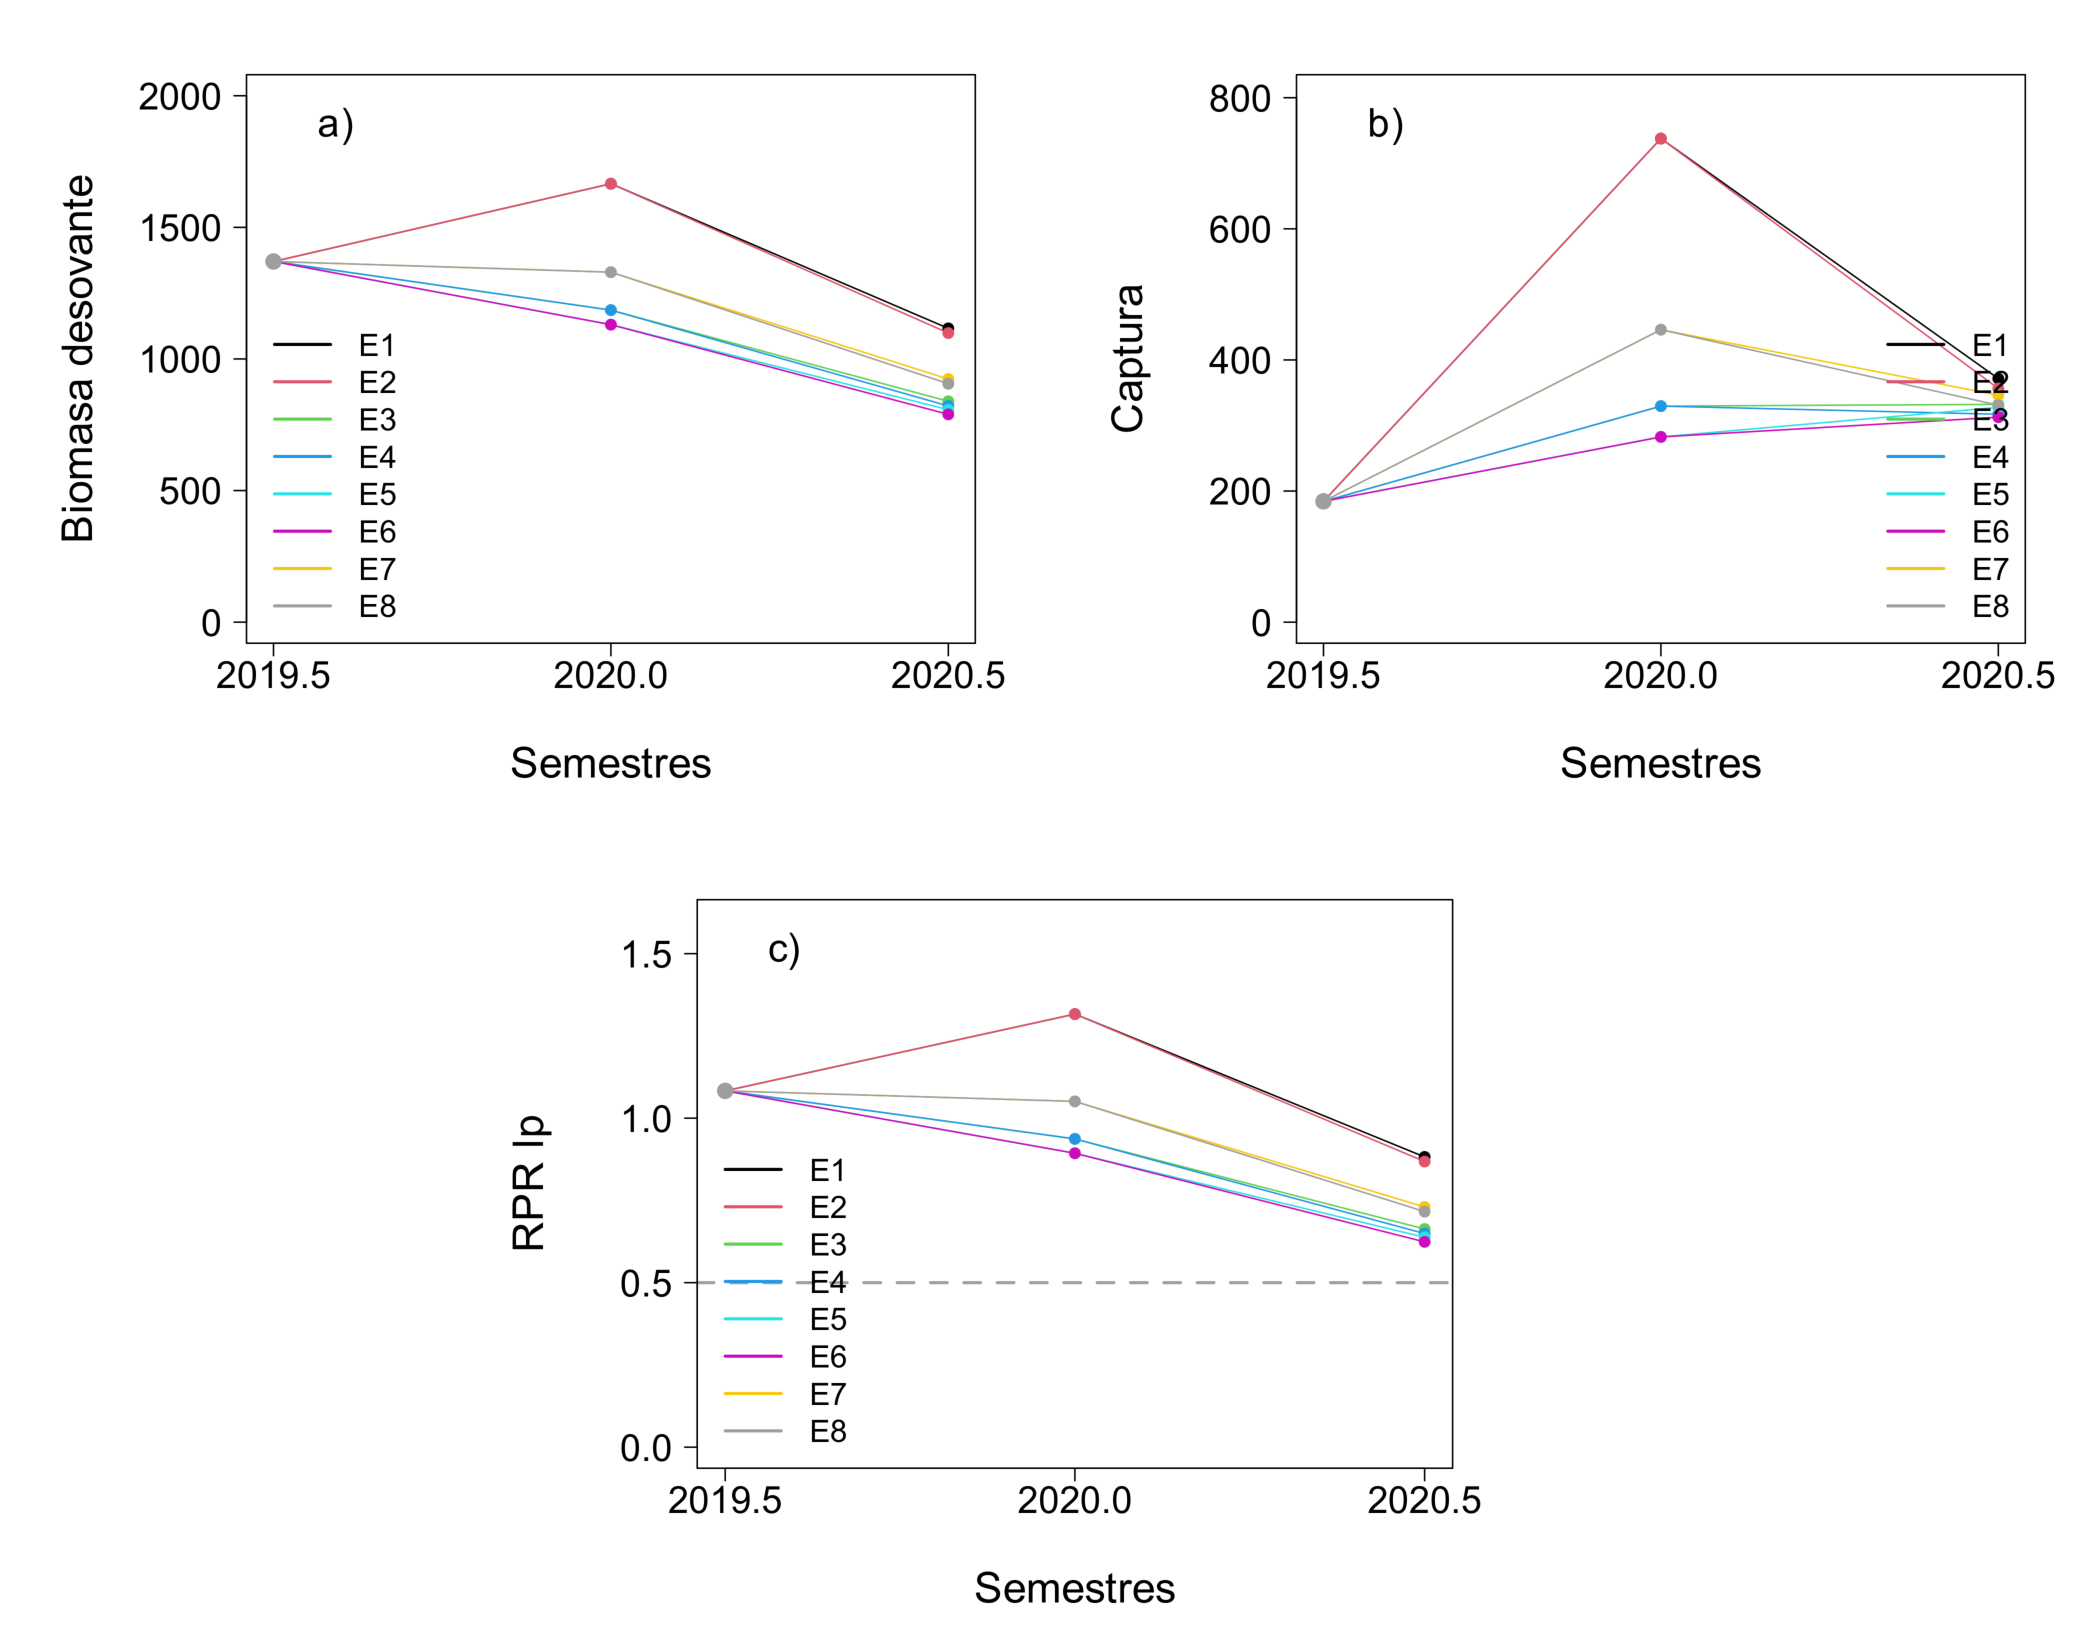
\includegraphics[width=13cm,height=11cm]{fig/figura22.pdf}
 \caption{Biomasa desovante (a), captura (b) y RPR largo plazao (c) proyectado para el segundo hito de asesor\'ia.}
 \label{Fig22}
\end{figure}
\vspace{0.5cm}


\vspace{0.5cm}
\begin{table}[htb!]
 \caption{CBA semestral proyectada (2020.0-2020.5) y anual para el 2020 para el stock de anchoveta dado el criterio del F=F$_{RMS}$ y los diferentes escenarios evaluados.}
 \label{Tab44}
 \centering
 \small
 \begin{tabular}{lccc}
 \hline\noalign{\vskip 0.1cm}
 Escenario & 2020.0 & 2020.5 & 2020$_{TOT}$ \\
 \hline\noalign{\vskip 0.1cm}
 E1  & 737.6 & 371.5 & 1109.2  \\
 E2  & 737.6 & 356.4 & 1094.0 \\
 E3  & 329.5 & 332.2 & 661.7 \\
 E4  & 329.5 & 317.1 & 646.6  \\
 E5  & 282.6 & 327.7 & 610.3  \\
 E6  & 282.6 & 312.6 & 595.2  \\
 E7  & 446.1 & 346.1 & 792.2  \\
 E8  & 446.0 & 330.9 & 776.9  \\
 \hline
 \end{tabular}
\end{table}
\vspace{0.5cm}

\pagebreak

\subsubsection{Aporte de cada grupo de edad a la captura proyectada por semestre}


Durante la proyecci\'on del stock de anchoveta se estim\'o la captura en
n\'umero de individuos por grupo de edad (Baranov, 1918), y luego fue
dividida por la suma total de todos los grupos de edad. Este porcentaje
por grupo de edad en la captura es presentado en las
\textbf{Tabla \ref{Tab45}}, \textbf{Tabla \ref{Tab46}}, \textbf{Tabla \ref{Tab47}},
\textbf{Tabla \ref{Tab48}}, \textbf{Tabla \ref{Tab49}}, \textbf{Tabla \ref{Tab50}},
\textbf{Tabla \ref{Tab51}} y \textbf{Tabla \ref{Tab52}} para el
escenario E1, E2, E3, E4, E5, E6, E7 y E8 respectivamente. Independiente del escenario
evaluado, el grupo de edad 1 (6 meses) es que mayor porcentaje aporta a
la captura semestral. Para el escenario E1 y E2 este valor varia entre
un 89\% y un 80\%, para el escenario E3 y E4 este valor varia entre un
75\% y un 84\%., para el escenario E5 y E6 este valor varia entre un 71\% y un 85\% y
para el escenario E7 y E8 este valor varia entre un 82\% y 83\%. En general, los grupos
de edades 0 (reclutas), 1 (6 meses) y 2 (1 a\~{n}o) aportan el 100\% de la captural
semestral para los diferentes escenarios evaluados.\\

\vspace{0.5cm}
\begin{table}[htb!]
 \caption{Porcentaje por grupo de edad en la captura proyectada (2020) para el escenario E1.}
 \label{Tab45}
 \centering
 \small
 \begin{tabular}{lcc}
 \hline\noalign{\vskip 0.1cm}
 Edad & 2020.0 & 2020.5 \\
 \hline\noalign{\vskip 0.1cm}
 0 & 0.052 & 0.119  \\
 \rowcolor{Gray}
 1 & 0.894 & 0.804 \\
 2 & 0.051 & 0.073 \\
 3 & 0.001 & 0.002  \\
 \hline
 \rowcolor{Gray}
 Suma(0:2) & 0.998 & 0.997 \\
 \hline
 \end{tabular}
\end{table}
\vspace{0.5cm}



\vspace{0.5cm}
\begin{table}[htb!]
 \caption{Porcentaje por grupo de edad en la captura proyectada (2020) para el escenario E2.}
 \label{Tab46}
 \centering
 \small
 \begin{tabular}{lcc}
 \hline\noalign{\vskip 0.1cm}
 Edad & 2020.0 & 2020.5 \\
 \hline\noalign{\vskip 0.1cm}
 0 & 0.050 & 0.117  \\
 \rowcolor{Gray}
 1 & 0.896 & 0.802 \\
 2 & 0.051 & 0.076 \\
 3 & 0.001 & 0.002  \\
 \hline
 \rowcolor{Gray}
 Suma(0:2) & 0.998 & 0.997 \\
 \hline
 \end{tabular}
\end{table}
\vspace{0.5cm}



\vspace{0.5cm}
\begin{table}[htb!]
 \caption{Porcentaje por grupo de edad en la captura proyectada (2020) para el escenario E3.}
 \label{Tab47}
 \centering
 \small
 \begin{tabular}{lcc}
 \hline\noalign{\vskip 0.1cm}
 Edad & 2020.0 & 2020.5 \\
 \hline\noalign{\vskip 0.1cm}
 0 & 0.120 & 0.119  \\
 \rowcolor{Gray}
 1 & 0.759 & 0.849 \\
 2 & 0.117 & 0.028 \\
 3 & 0.002 & 0.002  \\
 \hline
 \rowcolor{Gray}
 Suma(0:2) & 0.997 & 0.997 \\
 \hline
 \end{tabular}
\end{table}
\vspace{0.5cm}



\vspace{0.5cm}
\begin{table}[htb!]
 \caption{Porcentaje por grupo de edad en la captura proyectada (2020) para el escenario E4.}
 \label{Tab48}
 \centering
 \small
 \begin{tabular}{lcc}
 \hline\noalign{\vskip 0.1cm}
 Edad & 2020.0 & 2020.5 \\
 \hline\noalign{\vskip 0.1cm}
 0 & 0.115 & 0.123  \\
 \rowcolor{Gray}
 1 & 0.763 & 0.843 \\
 2 & 0.118 & 0.080 \\
 3 & 0.002 & 0.002  \\
 \hline
 \rowcolor{Gray}
 Suma(0:2) & 0.997 & 0.997 \\
 \hline
 \end{tabular}
\end{table}
\vspace{0.5cm}


\vspace{0.5cm}
\begin{table}[htb!]
 \caption{Porcentaje por grupo de edad en la captura proyectada (2020) para el escenario E5.}
 \label{Tab49}
 \centering
 \small
 \begin{tabular}{lcc}
 \hline\noalign{\vskip 0.1cm}
 Edad & 2020.0 & 2020.5 \\
 \hline\noalign{\vskip 0.1cm}
 0 & 0.141 & 0.119  \\
 \rowcolor{Gray}
 1 & 0.717 & 0.854 \\
 2 & 0.137 & 0.023 \\
 3 & 0.003 & 0.002  \\
 \hline
 \rowcolor{Gray}
 Suma(0:2) & 0.995 & 0.996 \\
 \hline
 \end{tabular}
\end{table}
\vspace{0.5cm}


\vspace{0.5cm}
\begin{table}[htb!]
 \caption{Porcentaje por grupo de edad en la captura proyectada (2020) para el escenario E6.}
 \label{Tab50}
 \centering
 \small
 \begin{tabular}{lcc}
 \hline\noalign{\vskip 0.1cm}
 Edad & 2020.0 & 2020.5 \\
 \hline\noalign{\vskip 0.1cm}
 0 & 0.135 & 0.124  \\
 \rowcolor{Gray}
 1 & 0.722 & 0.848 \\
 2 & 0.138 & 0.024 \\
 3 & 0.003 & 0.002  \\
 \hline
 \rowcolor{Gray}
 Suma(0:2) & 0.995 & 0.996 \\
 \hline
 \end{tabular}
\end{table}
\vspace{0.5cm}


\vspace{0.5cm}
\begin{table}[htb!]
 \caption{Porcentaje por grupo de edad en la captura proyectada (2020) para el escenario E7.}
 \label{Tab51}
 \centering
 \small
 \begin{tabular}{lcc}
 \hline\noalign{\vskip 0.1cm}
 Edad & 2020.0 & 2020.5 \\
 \hline\noalign{\vskip 0.1cm}
 0 & 0.089 & 0.119  \\
 \rowcolor{Gray}
 1 & 0.822 & 0.836 \\
 2 & 0.086 & 0.041 \\
 3 & 0.001 & 0.002  \\
 \hline
 \rowcolor{Gray}
 Suma(0:2) & 0.997 & 0.996 \\
 \hline
 \end{tabular}
\end{table}
\vspace{0.5cm}


\vspace{0.5cm}
\begin{table}[htb!]
 \caption{Porcentaje por grupo de edad en la captura proyectada (2020) para el escenario E8.}
 \label{Tab52}
 \centering
 \small
 \begin{tabular}{lcc}
 \hline\noalign{\vskip 0.1cm}
 Edad & 2020.0 & 2020.5 \\
 \hline\noalign{\vskip 0.1cm}
 0 & 0.085 & 0.122  \\
 \rowcolor{Gray}
 1 & 0.825 & 0.831 \\
 2 & 0.087 & 0.043 \\
 3 & 0.001 & 0.002  \\
 \hline
 \rowcolor{Gray}
 Suma(0:2) & 0.997 & 0.996 \\
 \hline
 \end{tabular}
\end{table}
\vspace{0.5cm}


\subsubsection{Abundancia semestral proyectada}


En las \textbf{Tabla \ref{Tab53}}, \textbf{Tabla \ref{Tab54}},
\textbf{Tabla \ref{Tab55}} y \textbf{Tabla \ref{Tab56}} se presentan las
matrices de abundancia en n\'umero durante la proyecci\'on del stock de
anchoveta. En estas se observan los diferentes supuestos
(\textbf{Tabla \ref{Tab6}}) aplicados para cada uno de los casos
evaluados. Adem\'as, se muestra la abundancia por grupo de edad al \'ultimo
semestre estimado por el modelo de evaluaci\'on, de manera de identificar
el \'ultimo reclutamiento estimado (\textbf{Tabla \ref{Tab53}} y
\textbf{Tabla \ref{Tab54}}). Y en las tablas siguientes se muestra el
reclutamiento penalizado por los diferentes m\'etodos para el semestre 2019.5.\\




\vspace{0.5cm}
\begin{table}[htb!]
 \caption{Abundancia semestral proyectada (2019.5 - 2020.5) para el escenario E1.}
 \label{Tab53}
 \centering
 \small
 \begin{tabular}{lrrr}
 \hline\noalign{\vskip 0.1cm}
 Edad & 2019.5 & 2020.0 & 2020.5 \\
 \hline\noalign{\vskip 0.1cm}
 0 & \cellcolor{Gray1}498.17 & \cellcolor{Gray2}239.04 & \cellcolor{Gray3}283.16 \\
 1 & 111.22 & \cellcolor{Gray1}165.00 & \cellcolor{Gray2}77.55 \\
 2 & 26.66 & 31.30 & \cellcolor{Gray1}23.24 \\
 3 & 8.57 & 8.52 & 8.49  \\
 4 & 1.89 & 2.84 & 2.79 \\
 5 & 0.48 & 0.79 & 1.21 \\
 \hline
 \end{tabular}
\end{table}
\vspace{0.5cm}



\vspace{0.5cm}
\begin{table}[htb!]
 \caption{Abundancia semestral proyectada (2019.5 - 2020.5) para el escenario E2.}
 \label{Tab54}
 \centering
 \small
 \begin{tabular}{lrrr}
 \hline\noalign{\vskip 0.1cm}
 Edad & 2019.5 & 2020.0 & 2020.5 \\
 \hline\noalign{\vskip 0.1cm}
 0 & \cellcolor{Gray1}498.17 & \cellcolor{Gray2}227.26 & \cellcolor{Gray3}265.29 \\
 1 & 111.22 & \cellcolor{Gray1}165.00 & \cellcolor{Gray2}73.73 \\
 2 & 26.66 & 31.30 & \cellcolor{Gray1}23.24 \\
 3 & 8.57 & 8.52 & 8.49  \\
 4 & 1.89 & 2.84 & 2.79 \\
 5 & 0.48 & 0.79 & 1.21 \\
 \hline
 \end{tabular}
\end{table}
\vspace{0.5cm}



\vspace{0.5cm}
\begin{table}[htb!]
 \caption{Abundancia semestral proyectada (2019.5 - 2020.5) para el escenario E3.}
 \label{Tab55}
 \centering
 \small
 \begin{tabular}{lrrr}
 \hline\noalign{\vskip 0.1cm}
 Edad & 2019.5 & 2020.0 & 2020.5 \\
 \hline\noalign{\vskip 0.1cm}
 0 & \cellcolor{Gray1}185.15 & \cellcolor{Gray2}239.04 & \cellcolor{Gray3}267.53 \\
 1 & 111.22 & \cellcolor{Gray1}61.44 & \cellcolor{Gray2}77.55 \\
 2 & 26.66 & 31.30 & \cellcolor{Gray1}8.65 \\
 3 & 8.57 & 8.52 & 8.49  \\
 4 & 1.89 & 2.84 & 2.79 \\
 5 & 0.48 & 0.79 & 1.21 \\
 \hline
 \end{tabular}
\end{table}
\vspace{0.5cm}



\vspace{0.5cm}
\begin{table}[htb!]
 \caption{Abundancia semestral proyectada (2019.5 - 2020.5) para el escenario E4.}
 \label{Tab56}
 \centering
 \small
 \begin{tabular}{lrrr}
 \hline\noalign{\vskip 0.1cm}
 Edad & 2019.5 & 2020.0 & 2020.5 \\
 \hline\noalign{\vskip 0.1cm}
 0 & \cellcolor{Gray1}185.15 & \cellcolor{Gray2}227.26 & \cellcolor{Gray3}265.29 \\
 1 & 111.22 & \cellcolor{Gray1}61.44 & \cellcolor{Gray2}73.73 \\
 2 & 26.66 & 31.30 & \cellcolor{Gray1}8.65 \\
 3 & 8.57 & 8.52 & 8.49  \\
 4 & 1.89 & 2.84 & 2.79 \\
 5 & 0.48 & 0.79 & 1.21 \\
 \hline
 \end{tabular}
\end{table}
\vspace{0.5cm}



\vspace{0.5cm}
\begin{table}[htb!]
 \caption{Abundancia semestral proyectada (2019.5 - 2020.5) para el escenario E5.}
 \label{Tab57}
 \centering
 \small
 \begin{tabular}{lrrr}
 \hline\noalign{\vskip 0.1cm}
 Edad & 2019.5 & 2020.0 & 2020.5 \\
 \hline\noalign{\vskip 0.1cm}
 0 & \cellcolor{Gray1}149.52 & \cellcolor{Gray2}239.04 & \cellcolor{Gray3}265.73 \\
 1 & 111.22 & \cellcolor{Gray1}49.52 & \cellcolor{Gray2}77.55 \\
 2 & 26.66 & 31.30 & \cellcolor{Gray1}6.97 \\
 3 & 8.57 & 8.52 & 8.49  \\
 4 & 1.89 & 2.84 & 2.79 \\
 5 & 0.48 & 0.79 & 1.21 \\
 \hline
 \end{tabular}
\end{table}
\vspace{0.5cm}




\vspace{0.5cm}
\begin{table}[htb!]
 \caption{Abundancia semestral proyectada (2019.5 - 2020.5) para el escenario E6.}
 \label{Tab58}
 \centering
 \small
 \begin{tabular}{lrrr}
 \hline\noalign{\vskip 0.1cm}
 Edad & 2019.5 & 2020.0 & 2020.5 \\
 \hline\noalign{\vskip 0.1cm}
 0 & \cellcolor{Gray1}149.52 & \cellcolor{Gray2}227.26 & \cellcolor{Gray3}265.29 \\
 1 & 111.22 & \cellcolor{Gray1}49.52 & \cellcolor{Gray2}73.73 \\
 2 & 26.66 & 31.30 & \cellcolor{Gray1}6.97 \\
 3 & 8.57 & 8.52 & 8.49  \\
 4 & 1.89 & 2.84 & 2.79 \\
 5 & 0.48 & 0.79 & 1.21 \\
 \hline
 \end{tabular}
\end{table}
\vspace{0.5cm}



\vspace{0.5cm}
\begin{table}[htb!]
 \caption{Abundancia semestral proyectada (2019.5 - 2020.5) para el escenario E7.}
 \label{Tab59}
 \centering
 \small
 \begin{tabular}{lrrr}
 \hline\noalign{\vskip 0.1cm}
 Edad & 2019.5 & 2020.0 & 2020.5 \\
 \hline\noalign{\vskip 0.1cm}
 0 & \cellcolor{Gray1}274.19 & \cellcolor{Gray2}241.18 & \cellcolor{Gray3}274.28 \\
 1 & 111.22 & \cellcolor{Gray1}90.81 & \cellcolor{Gray2}78.25 \\
 2 & 26.66 & 31.58 & \cellcolor{Gray1}12.79 \\
 3 & 8.57 & 8.60 & 8.56  \\
 4 & 1.89 & 2.87 & 2.81 \\
 5 & 0.48 & 0.79 & 1.22 \\
 \hline
 \end{tabular}
\end{table}
\vspace{0.5cm}



\vspace{0.5cm}
\begin{table}[htb!]
 \caption{Abundancia semestral proyectada (2019.5 - 2020.5) para el escenario E8.}
 \label{Tab60}
 \centering
 \small
 \begin{tabular}{lrrr}
 \hline\noalign{\vskip 0.1cm}
 Edad & 2019.5 & 2020.0 & 2020.5 \\
 \hline\noalign{\vskip 0.1cm}
 0 & \cellcolor{Gray1}274.19 & \cellcolor{Gray2}229.29 & \cellcolor{Gray3}267.67 \\
 1 & 111.22 & \cellcolor{Gray1}90.81 & \cellcolor{Gray2}74.39 \\
 2 & 26.66 & 31.58 & \cellcolor{Gray1}12.79 \\
 3 & 8.57 & 8.60 & 8.56  \\
 4 & 1.89 & 2.87 & 2.81 \\
 5 & 0.48 & 0.79 & 1.22 \\
 \hline
 \end{tabular}
\end{table}
\vspace{0.5cm}


\pagebreak

\clearpage
\newpage


\section{CONCLUSIONES}

\quad

Este reporte t\'ecnico dio cuenta de una revisi\'on de la estimaci\'on de la Captura
Biol\'ogicamente Aceptable (CBA) proyectada (4 a 2 semestres)
para los diferentes hitos de asesor\'ias que ocurren durante el establecimiento de la CBA anual,
una en forma preliminar en octubre y su actualizaci\'on en abril. Durante la proyecci\'on
del stock de anchoveta se deben tomar algunos supuestos sobre los reclutamientos futuros
que deben ingresar en la proyecci\'on, y por otro lado, dada la alta incertidumbre de la
\'ultima estimaci\'on del reclutamiento hecha por el modelo de evaluaci\'on y el patr\'on
retrospectivo que presentan los reclutamientos, se hace necesario aplicar alg\'un m\'etodo para penalizar el \'ultimo reclutamiento estimado por el modelo de evaluaci\'on. En este sentido, se aplicaron tres m\'etodos para penalizar el \'ultimo reclutamiento, i) el l\'imite inferior de la \'ultima estimaci\'on del reclutamiento, ii) predicir el reclutamiento desde una relaci\'on entre el
reclutamiento y el desembarque, y iii) el l\'imte inferior de la \'ultima
estimaci\'on de la desviaci\'on de $R_{0}$.

La principal conclusi\'on de los resultados reportados en este informe indican que para el
primer hito del establecimiento de la CBA (4 semestres proyectados), la CBA depende principalmente
de los niveles de reclutamiento promedios (longitud de la serie) que ingresan durante la proyecci\'on. Mientras que para el segundo hito de asesor\'ia (2 semestres proyectados), la CBA depende 
principalmente si el \'ultimo reclutamiento estimado por el modelo de evaluaci\'on es penalizado o no. 
Los resultados provenientes de la proyecci\'on para tres semestres indican una alta incertidumbre
y un alto valor para el \'ultimo reclutamiento estimado por el modelo de evaluaci\'on, casi cuatro
veces m\'as que la estimaci\'on hecha para cuatro semestre proyectados.

Finalmente, de los tres m\'etodos usados para penalizar el \'ultimo reclutamiento estimado por el
modelo de evaluaci\'on, el m\'etodo basado en la relaci\'on entre los desembarques y reclutas estima reclutamientos m\'as similares a los que son estimado por el modelo de evaluaci\'on cuando se incorpora nueva informaci\'on al modelo. Incluso, el l\'imite inferior del \'ultimo reclutamiento estimado por
el modelo de evaluaci\'on tiende a un valor por sobre el valor que es estimado cuando se agrega
nueva informaci\'on al modelo de evaluaci\'on (\textbf{Figura \ref{Fig14}}).


\pagebreak

\section{REFERENCIAS BIBLIOGR\'AFICAS}

\quad


Bertrand, A., M. Segura, M. Guiti\'errez y L. V\'asquez. 2004. From
small-scale habitat loopholes to decadal cycles: a habitat-based
hypothesis explaining fluctuation in pelagic fish populations off Peru.
\textit{Fish Fish.}, 5: 296-316.

Baranov, F.I. 1918. On the question of the biological basis of
fisheries,
\textit{Nauchnye Issledovaniya Ikhtiologicheskii Instituta Izvestiya},
vol.~1, 81-128 pp.

Beverton, R.J.H. y S.J. Holt. 1957. On the dynamics of exploited fish
populations. \textit{Fish. Invest. Ser.} 2, 19, 533 pp.


B\"ohm, G., C. Hern\'andez, G. P\'erez, E. D\'iaz, L. Cortez, L. Ossa, F. Cerna,
C. Valero, C. Machuca, L. Mu\~{n}oz, H. Reyes, M. Troncoso, C. Gaspar, Z.
Young y R. Aravena. 2013. Asesor\'ia integral para la toma de decisiones
en pesca y acuicultura, 2013. Actividad 1: Recursos pel\'agicos: Pesquer\'ia
Recursos pel\'agicos Zona Norte. Subsecretaria de Econom\'ia. Informe Final.
267 pp.

B\"ohm, G., C. Hern\'andez, E. D\'iaz, R. Ojeda, F. Cerna, C. Valero, C.
Machuca, L. Mu\~{n}oz, C. Rozas, H. Reyes, M. Pizarro, R. Aravena, M.
Troncoso, C. Gaspar y Z. Young. 2016. Programa de Seguimiento de las
Pesquer\'ias Pel\'agicas Zona Norte. Subsecretaria de Econom\'ia y EMT.
Informe Final. 364 pp.


Castillo, J. A. Saavedra, C. Hern\'andez, V. Catasti, F. Leiva, J.
Letelier, H. Reyes, M. Pizarro, B. Leiva, F. Cerna, A. L\'opez, L.
Herrera, G. Claramunt, A. Mujica y E. Uribe. 2009. Evaluaci\'on
hidroac\'ustica reclutamiento anchoveta entre la XV y IV Regiones, a\~{n}o
2009. Informe Final. FIP 2008-02. 285 pp + Figuras, Tablas y Anexos.

Castillo, J. A. Saavedra, F. Leiva, H. Reyes, M. Pizarro, F. Esp\'indola,
V. Catasti, C. Lang, C. Hern\'andez, B. Leiva, F. Cerna, A. L\'opez, L.
Herrera, G. Claramunt, E. Oliva, P. Moreno y M. Medina. 2010. Evaluaci\'on
hidroac\'ustica del reclutamiento de anchoveta en la XV, I y II Regiones,
a\~{n}o 2010. Informe Final. FIP 2009-02. 225 pp + Figuras, Tablas y Anexos.

Castillo, J. A. Saavedra, F. Leiva, H. Reyes, M. Pizarro, V. Catasti, C.
Lang, M., San Martin, B. Leiva, F. Cerna, A. L\'opez y L. Herrera. 2011.
Evaluaci\'on hidroac\'ustica del reclutamiento de anchoveta en la XV, I y II
Regiones, a\~{n}o 2011. Informe Final. FIP 2010-13. 248 pp + Figuras, Tablas
y Anexos.

Castillo, J. A. Saavedra, F. Leiva, H. Reyes, M. Pizarro, V. Catasti, C.
Lang, M., San Martin, B. Leiva, F. Cerna, A. L\'opez y L. Herrera. 2012.
Evaluaci\'on hidroac\'ustica del reclutamiento de anchoveta en la XV, I y II
Regiones, a\~{n}o 2012. Informe Final. FIP 2010-13. 248 pp + Figuras, Tablas
y Anexos.

Castillo, J. A. Saavedra, F. Leiva, H. Reyes, M. Pizarro, V. Catasti, C.
Lang, M., San Martin, B. Leiva, F. Cerna, A. L\'opez y L. Herrera. 2013.
Evaluaci\'on hidroac\'ustica del reclutamiento de anchoveta en la XV, I y II
Regiones, a\~{n}o 2013. Pre-Informe Final. FIP 2012-11. 248 pp + Figuras,
Tablas y Anexos.

Cerna, F. y G. Plaza. 2016. Daily growth patterns of juveniles and
adults of the Peruvian anchovy (Engraulis ringens) in northern Chile.
\textit{Mar. Fresh. Res.}, \href{http://dx.doi.org/10.1071/MF15032}.


Claramunt, G., Herrera, G., Moreno, P. y Azocar, C. 2014. Evaluaci\'on de
la biomasa desovante de anchoveta en la XV, I y II Regiones, A\~{n}o 2013.
Pre-Informe Final. FIP 2013-06.


Leiva, F., R. Vargas, C. Grendi, U. Cifuentes, C. Rozas, B. Leiva, F.
Cerna, A. L\'opez, C. Lang, L. Herrera, J. Jaque, J. Angulo y V.
Valenzuela. 2016. Evaluaci\'on hidroac\'ustica del reclutamiento de
anchoveta en la XV, I y II Regiones, a\~{n}o 2015. Informe Final, IFOP, 335
pp.


Mohn, R.K. 1993. Bootstrap estimates of ADAPT parameters, their projection
in risk analysis and the retrospective patterns. In: Risk Evaluation and
Biological Reference Points for Fisheries Management, pp. 173-184. Ed. by
S.J. Smith, J.J. Hunt and D. Rivard. Canadian Special Population Fisheries
and Aquatic Science 120.

Mohn, R. 1999. The retrospective problem in sequential population analysis:
An investigation using cod fishery and simulated data. ICES Journal of Marine
Science, 56: 473-488.


Parma, A.N. 1993. Retrospective catch-at-age analysis of pacific halibut:
implications on assessment of harvesting polices. In: Proceeding of the
International Symposium on Management Strategies for Exploited Fish
Populations, pp 247-265. Ed. by G. Kruse, D.M. Eggers, C. Pautzke,
R.J. Marasco and T.J. Quinn II. Alaska Sea Grant College Program.

Pay\'a I, C. Canales, D. Bucarey, M. Canales, F. Contreras, F. Esp\'indola,
E. Leal, R. Tascheri, A. Ya\~{n}ez y M.J. Z\'u\~{n}iga. 2014. Proyecto 2.16:
Revisi\'on de los puntos biol\'ogicos de referencia (Rendimiento M\'aximo
Sostenible) en las pesquer\'ias nacionales. Convenio II: Estatus y
posibilidades de explotaci\'on biol\'ogicamente sustentables de los
principales recursos pesqueros nacionales a\~{n}o 2014. Informe Final.
Subsecretaria de Econom\'ia y EMT - IFOP. 51 pp.+ 4 Anexos.


Saetersdal, G. y J.E. Valdivia. 1964. Un estudio del crecimiento, tama\~{n}o
y reclutamiento de la anchoveta (\textit{Engraulis ringens J.}) basado en datos
de frecuencia de longitud. Instituto de Investigaci\'on de los Recursos
Marinos, La Punta, Callao, Per\'u. Boletin Nº 4, vol 1, 85-136 pp.


Serra, R. y C. Canales. 2013. Investigaci\'on del Estatus y Evaluaci\'on de
Estrategias de Explotaci\'on Sustentables 2013, de las Principales
Pesquer\'ias Chilenas. Actividad 1: Peces Pel\'agicos: Anchoveta y sardina
espa\~{n}ola XV, I y II Regiones. 2011. Informe Final.


Simpson, J. y R. Buzeta. 1967. El crecimiento y la edad de la anchoveta
(\textit{Engraulis ringens, Jenyns}) en Chile basado en estudios de
frecuencia de longitud. \textit{Bolet\'in Cient\'ifico}, Nº 3. IFOP. 56 pp.

Sinclair, A., D. Gascon, R. O'Boyle, D. Rivard and S. Gavaris. 1991.
Consistency of some northwest Atlantic groundfish stock assessment.
NAFO Scientific Council Studies, 16: 59-77.



\newpage
\pagestyle{empty}
\begin{tikzpicture}
\node[anchor=south west,inner sep=0] at (0,0) {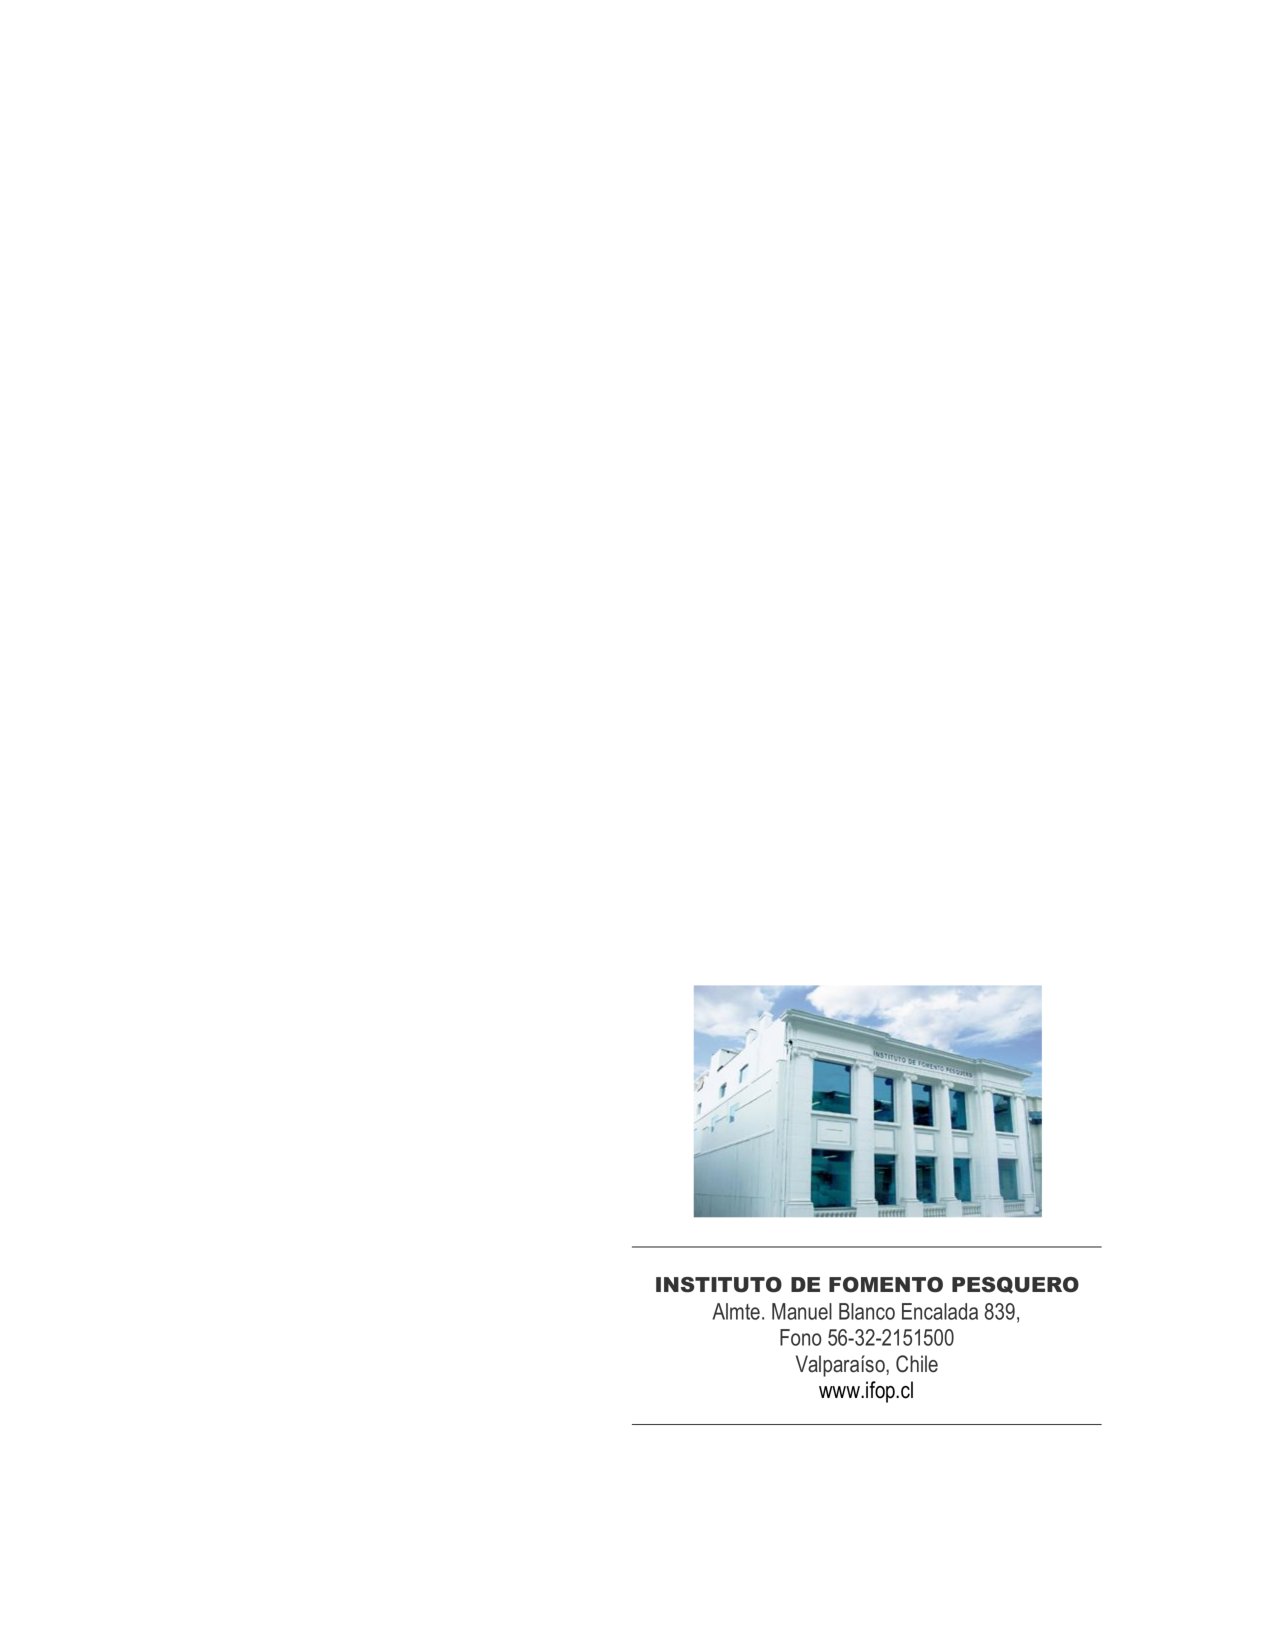
\includegraphics[height=22.3cm,width=22cm,viewport=70 74 318 698]{portada3.pdf}};
\end{tikzpicture}


\newpage
\begin{tikzpicture}
\node[anchor=south west,inner sep=0] at (0,0) {
\includegraphics[height=22.3cm,width=22cm,viewport=29 26 148 274]{portada4.pdf}};
%\node[anchor=south west,inner sep=0] at (0,0) {
\includegraphics[height=22.3cm,width=22cm,viewport=70 74 318 698]{portada4.pdf}};
\end{tikzpicture}




\end{document}
